\documentclass[a4paper]{book}

% hiperlinkovi - url i href
\usepackage{url}

% dodatne matematicke oznake
\usepackage{amssymb}
\usepackage{amsmath}
\usepackage{amsthm}

% jezicki paketi
\usepackage[serbian]{babel} % podrska za srpski jezik
\usepackage[utf8]{inputenc} % podrska za utf8 kodiranje

% izgled strane i boje
\usepackage[hmarginratio=1:1, bottom = 1.5in]{geometry}
\PassOptionsToPackage{svgnames}{xcolor}

% paketi za crtanje grafike
\usepackage{tikz}
\usetikzlibrary{intersections, calc, backgrounds, shapes.misc, arrows, petri, topaths, decorations.markings, automata, positioning}

% bojenje hiperlinkova
\usepackage[colorlinks=true, linkcolor=red!80, citecolor=green, urlcolor=blue]{hyperref}

% za podesavanje elemenata na strani
\usepackage{adjustbox}

% napredne figure i tabele
\usepackage{caption}
\usepackage{float}

% podesavanje hedera i futera
\usepackage{fancyhdr}	
\pagestyle{fancy}
\fancyhead{} 
\fancyhead[RO,RE]{\thepage}
\fancyhead[LO,LE]{\slshape \leftmark}
\fancyfoot{} 
\fancyfoot[C]{ }

% za napredne kodove - koristi se okruzenje "lstlisting"
\usepackage{listings}
% na pocetku svakog POGLAVLJA potrebno je pozvati narednu komandu
\newcommand{\setbookcodestyle}{
	\lstset{
		basicstyle=\ttfamily,
		columns=fullflexible,
		keepspaces=true,
		showstringspaces=false,
		escapechar=\%,
		tabsize=4,
		breaklines=true,
		postbreak=\mbox{\textcolor{red}{$\hookrightarrow$}\space},
		frame=None,
		keywordstyle=\color{black},
	   	commentstyle=\color{black},
	   	identifierstyle=\color{black},
	   	stringstyle=\color{black},
	   	numbers=left
	}
}
% na pocetku svake sekcije koja sadrzi KODOVE SA VEZBI potrebno je pozvati narednu komandu
\newcommand{\setexamplecodestyle}{
	\lstset{
		basicstyle=\ttfamily,
		columns=fullflexible,
		keepspaces=true,
		showstringspaces=false,
		escapechar=\%,
		tabsize=4,
		language=Python,
		breaklines=true,
		postbreak=\mbox{\textcolor{red}{$\hookrightarrow$}\space},
		frame=None,
	   	keywordstyle=\bfseries\color{green!40!black},
	   	commentstyle=\itshape\color{purple!40!black},
	   	identifierstyle=\color{blue},
	   	stringstyle=\color{orange}
	}
}

% dodatna okruzenja
\newtheorem{definicija}{Definicija}[chapter]
\newtheorem{teorema}[definicija]{Teorema}
\newtheorem{lema}[definicija]{Lema}
\newtheorem{primer}[definicija]{Primer}
\newtheorem{zadatak}[definicija]{Zadatak}
\newtheorem*{dokaz}{Dokaz}


\usepackage{mdframed}
\newtheorem{Problem}{Problem}
\newenvironment{problem}
{\begin{mdframed}\begin{Problem}}
		{\end{Problem}\end{mdframed}}

% dodatne komande
\newcommand{\blankpage}{\newpage\hbox{}\thispagestyle{empty}\newpage}
\renewcommand\qedsymbol{\hspace*{\stretch{1}} $\blacksquare$}
\usepackage{tcolorbox}
\begin{document}
\iffalse 
\begin{titlepage}
	\vspace*{0.4\textheight}
	
	\begin{center}
		{\Huge \textsc{Bioinformatika}}
	\end{center}
	
	\vfill
	
	\begin{center}
		{\Large \today.}
	\end{center}
\end{titlepage}

\blankpage

\frontmatter
\tableofcontents
\blankpage

\chapter*{Predgovor}
Tekst se sastoji od proširenih beleški sa predavanja na osnovu knjige Pavel A. Pevzner, Phillip Compeau: Bioinformatics Algorithms: An Active Learning Approach. \\Tekst su sastavili studenti sa kursa održanog u školskoj 2017/2018 godini: 
\begin{itemize}
	\item Una Stanković 1095/2016
	\item Marina Nikolić 1055/2017
	\item Strahinja Milojević 1049/2017
	\item Anja Bukurov 1082/2016
	\item Nikola Ajzenhamer 1083/2016
	\item Vojislav Stanković 1080/2016
	\item Milica Đurić 1084/2016
	\item Ana Stanković 1096/2016
	\item Aleksandra Branković 1057/2017
	\item Ljubica Aćimović 1027/2016
	\item Jasmina Vasilijević 1067/2017
	\item Anđela Mijailović 1050/2017
	\item Milena Dukanac 1020/2017
	\item Filip Miljaković 1040/2017
	\item Petar Kulezić 1058/2017
\end{itemize}


\blankpage
\fi 
\setbookcodestyle
\mainmatter
\chapter{Gde u genomu počinje replikacija genoma?}
\setbookcodestyle

\section{Uvod}
\label{sec:uvod}

Na samom početku, želimo da definišemo pojam bioinformatike i da pokušamo da shvatimo koji je njen osnovni cilj. Da bismo to postigli, pogledajmo tri definicije, iz različitih izvora:

\begin{itemize}
  \item $"$Bioinformatika je nauka koja se bavi prikupljanjem i analizom kompleksnih bioloških podataka poput genetskih kodova.$"$ - Oksfordski rečnik (engl. \textit{Oxford Dictionary})
  \item $"$Bioinformatika predstavlja prikupljanje, klasifikaciju, čuvanje i analizu biohemijskih i bioloških informacija korišćenjem računara, a posebno se primenjuje u molekularnoj genetici i genomici.$"$ - Rečnik Meriam-Vebster (engl. \textit{Merriam-Webster Dictionary}) 
 \item $"$Bioinformatika je interdisciplinarno polje koje radi na razvoju metoda i softverskih alata za razumevanje bioloških podataka.$"$ - Vikipedija (engl. \textit{Wikipedia}) 
\end{itemize}

\noindent Na osnovu ove tri definicije možemo zaključiti da: \textit{Bioinformatika predstavlja primenu računarskih tehnologija u istraživanjima u oblasti biologije i srodnih nauka.}\\\\
Bioinformatika ima široku primenu i njene primene rastu zajedno sa razvojem discipline. Kao što možemo videti na slici ispod, primena bioinformatike se može sagledati kroz personalizovanu medicinu. Naime, na osnovu prikupljene veće količine podataka i njihove analize, uz pomoć različitih računarskih metoda, na primer metoda veštačke inteligencije, možemo doći do informacija potrebnih da na najbolji način lečimo pacijenta ili mu odredimo terapiju koja će mu na najbolji, najbrži i najbezbolniji način pomoći da prevaziđe određene zdravstvene probleme.  \\

\iffalse
\begin{figure}[h]
\caption{Primena bioinformatike}
\centering
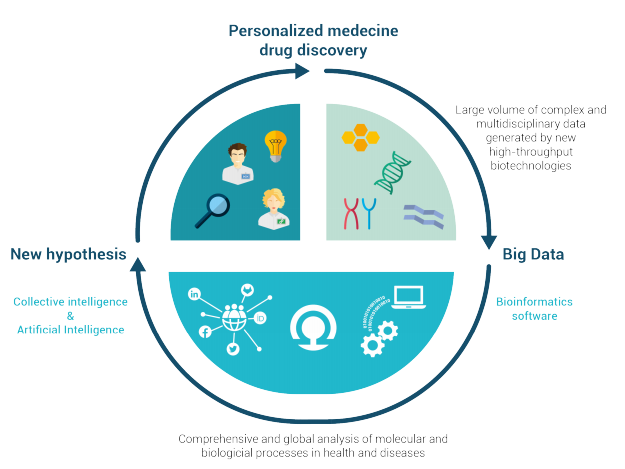
\includegraphics[width=0.7\textwidth]{poglavlja/1/slike/Primena.png}
\end{figure} 
\fi

\noindent Bioinformatika je spoj više različitih disciplina, kao što su:
statistika, istraživanje podataka, računarstvo, računarska biologija, biologija, biostatistika.
%Prikaz preklapanja ovih disciplina možemo videti na slici 1.2.

\iffalse 
\begin{figure}[h]
\caption{Preklapanjem različitih disciplina dobijamo bioinformatiku.}
\centering
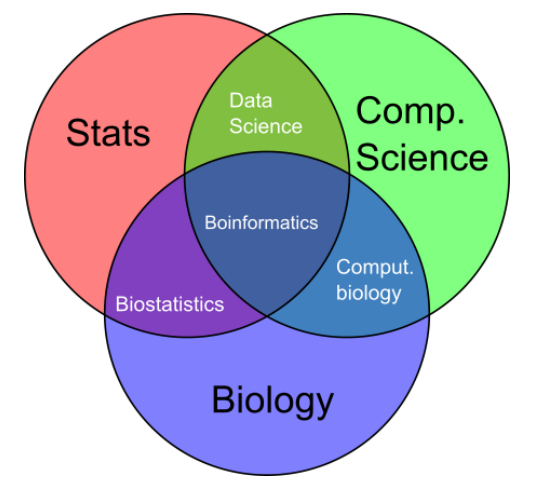
\includegraphics[width=0.7\textwidth]{poglavlja/1/slike/Multidisciplinarnost.png}
\end{figure}  
\fi 


\section{Replikacija genoma}
\label{sec:replikacija}

\subsection{DNK}

Dezoksiribonukleinska kiselina (akronimi DNK ili DNA, od engl.  \textit{deoxyribonucleic acid}) je nukleinska kiselina koja sadrži uputstva za razvoj i pravilno funkcionisanje svih živih organizama. Zajedno sa RNK i proteinima, DNK je jedan od tri glavna tipa makromolekula koji su esencijalni za sve poznate forme života. 
\\
\\
Sva živa bića svoj genetički materijal nose u obliku DNK, sa izuzetkom nekih virusa koji imaju ribonukleinsku kiselinu (RNK). DNK ima veoma važnu ulogu ne samo u prenosu genetičkih informacija sa jedne na drugu generaciju, već sadrži i uputstva za građenje neophodnih ćelijskih organela, proteina i RNK molekula. DNK segment koji sadrži ova važna uputstva se naziva gen.\\

DNK se sastoji iz dva polimerna lanca koji imaju antiparalelnu orijentaciju, i svaki od njih je sastavljen od azotnih baza:
\begin{itemize}
	\item adenin (A)
	\item timin (T)
	\item guanin (G)
	\item citozin (C)
\end{itemize}

\iffalse 
\begin{figure}[h]
\caption{Prikaz DNK, slika preuzeta sa https://ghr.nlm.nih.gov/primer/basics/dna}
\centering
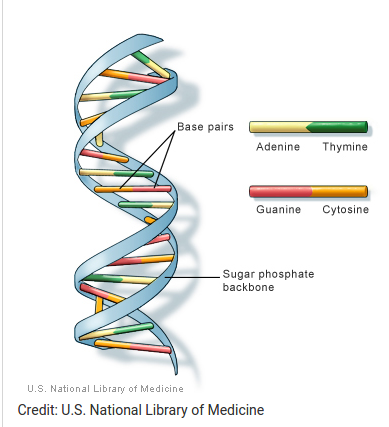
\includegraphics[width=0.5\textwidth]{poglavlja/1/slike/DNK.png}
\end{figure} 
\fi

Lanci DNK su međusobno spojeni i to tako da se veze uspostavljaju isključivo između adenina i timina ili između guanina i citozina. Na osnovu toga, ako nam je poznat sastav jednog lanca, lako možemo zakljuciti i sastav drugog lanca, zbog čega se kaže da su DNK lanci \textbf{međusobno komplementarni}.\\\\
Da bismo lakše manipulisali sa informacijama koje DNK nosi i približili sadržaj računarskoj struci, DNK ćemo posmatrati kao nisku nad azbukom \{A, C, G, T\}.

\subsection{Replikacija genoma u ćeliji}
Replikacija genoma je jedan od najvažnijih zadataka ćelije. Pre nego što se podeli, ćelija mora da najpre replicira svoj genom, tako da svaka od ćerki ćelija dobije svoju kopiju. \\\\
Džejms Votson (engl. \textit{James Watson}) i Fransis Krik (engl. \textit{Fransis Crick}) su 1953. godine napisali rad u kome su primetili da postoji mehanizam za kopiranje genetskog materijala. Oni su uočili da se lanci roditeljskog DNK molekula odvijaju tokom replikacije i da se, potom, svaki lanac ponaša kao uzorak za sintezu novog lanca (na osnovu toga što se uvek spajaju iste aminokiseline A-T i G-C, rekreiranje lanca je moguće). Kao rezultat ovakvog ponašanja, proces replikacije počinje parom komplementarnih lanca i završava se sa dva para komplementarnih lanaca, kao što se može videti na slici ispod.\\\\

\iffalse 
\begin{figure}[h]
\centering
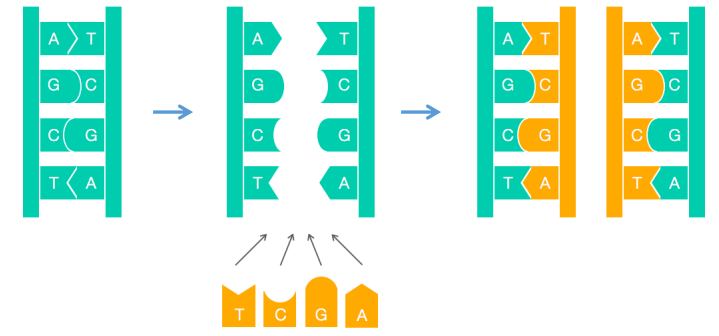
\includegraphics[width=1\textwidth]{poglavlja/1/slike/Replikacija.png}
\caption{Prikaz replikacije}
\end{figure} 
\fi 

Replikacija počinje u regionu genoma koji se naziva \textbf{početni region replikacije} (skraćeno \textit{oriC}), izvode je enzimi koje se nazivaju DNK polimeraze, koje predstavljaju mašine za kopiranje na molekularnom nivou.\\\\
Nalaženje početnog regiona replikacije predstavlja veoma važan problem, ne samo za razumevanje funkcionisanja kako se ćelije repliciraju, već je koristan i u raznim biomedicinskim problemima. Na primer, neki metodi genskih terapija uključuju genetski izmenjene mini genome, koji se zovu virusni vektori, zbog svoje sposobnosti da prodru kroz ćelijski zid (poput pravih virusa). Virusni vektori u sebi nose veštačke gene koji unapređuju postojeći genom. Genska terapija je prvi put uspešno izvršena 1990. godine na devojčici koja je bila toliko otporna na infekcije da je bila primorana da živi isključivo u sterilnom okruženju.
\\
\\
Osnovna ideja genske terapije je da se pacijent, koji pati od nedostatka nekog bitnog gena, zarazi virusnim vektorom koji sadrži veštački gen koji enkodira terapeutski protein. Jednom kad je unutar ćelije, vektor se replicira, što dovodi do lečenja bolesti pacijenta. Da bi moglo da dođe do ovoga, biolozima je neophodno da znaju gde je \textit{oriC}.

Pitamo se kako ćelija prepoznaje oriC? Sigurno je da postoji neka niska aminokiselina koja označava oriC, ali kako ga prepoznati? Ograničimo se na bakterijski genom, koji se sastoji od jednog kružnog hromozoma. Istraživanje je pokazalo da je region, koji predstavlja oriC kod bakterija,
dug svega nekoliko stotina nukleotida.
\\
\\
\iffalse
\begin{figure}[h]
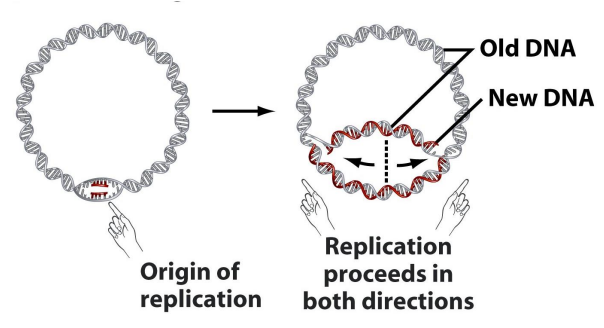
\includegraphics[width=0.7\textwidth]{poglavlja/1/slike/Replikacija_bakterija.png}
\caption{Prikaz početka replikacije kod bakterija}
\centering
\end{figure} 
\fi 
Poznato je da DNKA utiče na početak replikacije. \textit{DNKA} je protein koji se vezuje na kratki segment unutar oriC, poznatiji kao \textbf{DNKA boks}. Ona predstavlja poruku unutar sekvence DNK koja govori proteinu DNKA da se veže baš tu. Postavlja se pitanje kao pronaći taj region bez prethodnog poznavanja izgleda DNKA boks? \\\\

Da bismo bolje razumeli \textit{problem skrivene poruke} uzmimo za primer priču Edgara Alana Poa - $"$Zlatni jelenak$"$ (engl. \textit{$"$The Gold-Bug$"$}).
Naime, u toj priči jedan od likova, Vilijam Legrand (engl. \textit{William Legrand}), treba da dešifruje poruku :\\

\texttt{53++!305))6*;4826)4+.)4+);806*;48!8`6
0))85;]8*:+*8!83(88)5*!;46(;88*96*?;8\\
)*+(;485);5*!2:*+(;4956*2(5*4)8`8*;40
69285);)6!8)4++;1(+9;48081;8:8+1;48!8
5;4)\\485!528806*81(+9;48;(88;4(+?34;48
)4+;161;:188;+?;}\\\\
On uočava da se $"$;48$"$ pojavljuje veoma često, i da verovatno predstavlja $"$THE$"$, najčešću reč u engleskom jeziku. Znajući to, zamenjuje karaktere odgovarajućim slovima i postepeno dešifruje celu poruku.\\\\
\texttt{53++!305))6*THE26)H+.)H+)806*THE
!E`60))E5;]E*:+*E!E3(EE)5*!TH6(T
EE*96*?;E)*+\\(THE5)T5*!2:*+(TH956
*2(5*H)E`E*TH0692E5)T)6!E)H++T1(
+9THE0E1TE:E+1\\THE!E5T4)HE5!52880
6*E1(+9THET(EETH(+?34THE)H+T161T
:1EET+?T}\\\\
Želeli bismo da ovaj princip primenimo na naš problem nalaska \textit{oriC}-a. Ideja je da uvidimo da li postoje reči koje se neuobičajeno često pojavljuju. Uvedimo termin k-gram da označimo string dužine $k$ i COUNT(Text, Pattern) da označimo broj puta kojih se k-gram $Pattern$ pojavio u tekstu $Text$. Osnovna ideja je da pomeramo prozor, iste dužine kao k-gram $Pattern$, niz tekst, usput proveravajući da li se pojavljuje $Pattern$ u nekome od njih. 

\begin{lstlisting}
PATTERNCOUNT(Text, Pattern)
	count = 0
	for i = 0 to |Text| - |Pattern|
		if Text(i,|Pattern|) = Pattern
			count = count + 1 
	return count
\end{lstlisting}
	
Za neki $Pattern$ kažemo da je on \textit{najčešći k-gram} u tekstu $Text$, ako je njegov $COUNT$ najveći među svim k-gramima. Na primer, \textbf{ACTAT} je najčešći 5-gram u tekstu 
\\
$Text$ = ACA\textbf{ACTAT}GCA\textbf{ACTAT}CGGGACA\textbf{ACTAT}CCT,
a \textbf{ATA} je najčešći 3-gram u \\ $Text$ = CG\textbf{ATATA}TCC\textbf{ATA}G.\\\\
Sada, problem pronalaska čestih reči možemo posmatrati kao računarski problem:\\
\begin{tcolorbox}
\textbf{Problem čestih reči:} Pronaći najčešće k-grame u niski karaktera.\\
\textit{Ulaz:} Niska Text i ceo broj k.\\
\textit{Izlaz:} Svi najčešći k-grami u niski Text.
\end{tcolorbox}
~\\
Osnovni algoritam za pronalazak čestih k-grama u stringu $Text$ proverava sve k-grame koji se pojavljuju u tom stringu (takvih k-grama ima $|Text|-k+1$) i potom izračunava koliko puta se svaki k-gram pojavljuje. Da bismo implementirali ovaj algoritam, moramo da izgenerišemo niz $COUNT$, gde je $COUNT(i) = COUNT(Text, Pattern)$ za $Pattern = Text(i,k)$.\\

\begin{lstlisting}
FrequentWords(Text, k)
	FrequentPatterns <- an empty set
	for i = 0 to |Text| - k
		Pattern <- the k-mer Text(i,k)
		COUNT(i) <- PatternCount(Text, Pattern)
	maxCount <- max value in array COUNT
	for i = 0 to |Text| - k
		if COUNT(i) = maxCount
			add Text(i,k) to FrequentPatterns
	remove duplicates from FrequentPatterns
	return FrequentPatterns
\end{lstlisting}

\noindent Pitamo se, sada, kolika je složenost ovakvog pristupa? Ovaj algoritam, iako uspešno nalazi ono što se od njega traži, nije najefikasniji. S obzirom na to da svaki k-gram zahteva $|Text|-k+1$ provera, svaki od njih zahteva i do $k$ poređenja, pa je broj koraka izvršavanja funkcije $PatternCount(Text, Pattern)$ zapravo $(|Text|-k+1)*k$. Osim toga, $FrequentWords$ mora pozvati $PatternCount$ $|Text|-k+1$ puta (po jednom za svaki k-gram teksta), tako da je ukupan broj koraka \textit{$(|Text|-k+1)*(|Text|-k+1)*k$}. Iz navedenog, možemo zaključiti da je ukupna cena izvršavanja algoritma $FrequentWords$ \textbf{$O(|Text|^2*k)$}.

\subsubsection{Primer: Pronalazak čestih reči kod bakterije \textit{Vibrio cholerae}} 

Posmatrajmo, najpre, tablicu najčešćih k-grama u \textit{oriC} regionu bakterije \textit{Vibrio cholerae}. Da li nam se čini da se neki k-grami pojavljuju neuobičajeno često?\\ 

\begin{figure}[h]
\centering
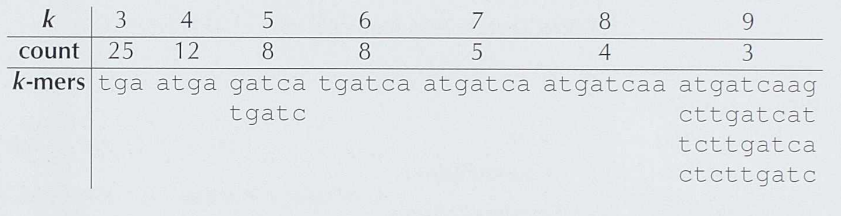
\includegraphics[width=1\textwidth]{poglavlja/1/slike/Tablica_VC.png}
\caption{Tablica najčešćih k-grama u \textit{oriC} regionu bakterije Vibrio cholerae}
\end{figure} 

Na primer, 9-gram \textbf{ATGATCAAG} se pojavljuje tri puta u \textit{oriC} regionu, da li nas to iznenađuje?\\

\begin{figure}[h]
\centering
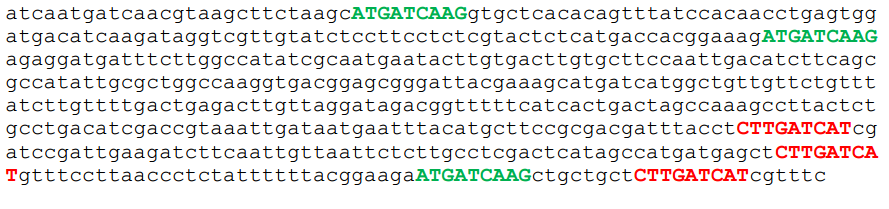
\includegraphics[width=1\textwidth]{poglavlja/1/slike/9_VC.png}
\caption{Prikaz 9-grama ATGATCAAG i njegovog komplementa u \textit{oriC} regionu Vibrio cholerae}
\end{figure} 

Označili smo najčešće 9-grame, umesto nekih drugih k-grama, jer je eksperimentima pokazano da su DNKA boksovi kod bakterija dugi 9 nukleotida. Uočimo da postoje četiri različita 9-grama koji se ponavljaju tri ili više puta u ovom regionu, to su: ATGATCAAG, CTTGATCAT, TCTTGATCA i CTCTTGATC.\\\\

Mala verovatnoća da se neki 9-gram toliko puta pojavi u \textit{oriC}-u kolere, govori nam da neki od četiri 9-grama koje smo pronašli može biti potencijalni DNKA boks, koji započinje replikaciju. Ali, koji?

Podsetimo se da nukleotidi A i T, kao i C i G, su komplementarni. Ako imamo jednu stranu lanca DNK i neke slobodne nukleotide, možemo lako zamisliti sintezu komplementarnog lanca, kao što se vidi na slici ispod. 

\iffalse 
\begin{figure}[h]
\caption{Komplementarni lanci se $"$kreću$"$ u suprotnim smerovima.}
\centering
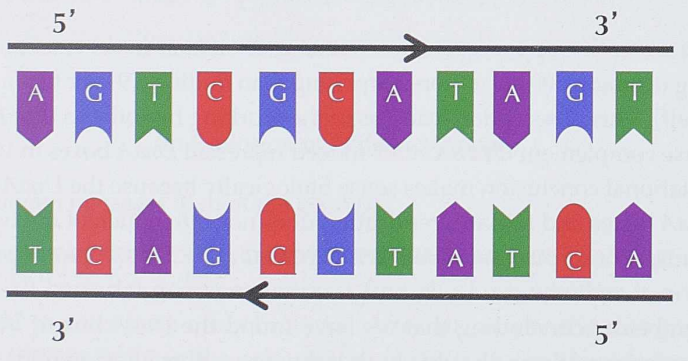
\includegraphics[width=1\textwidth]{poglavlja/1/slike/Komplementarni.png}
\end{figure} 
\fi 

Posmatrajmo ponovo sliku 1.7. Na njoj možemo uočiti 6 pojavljivanja niski ATGATCAAG i CTTGATCAT, koji su zapravo komplementarni. Naći 9-gram koji se pojavljuje 6 puta u DNK nisci dužine 500 nukleotida, je još više iznenađujuće, nego pronaći 9-gram koji se pojavljuje tri puta. Ovo posmatranje nas dovodi do toga da je ATGATCAAG (zajedno sa svojim komplementom) zaista DNKA boks Vibrio cholerae. Ovaj zaključak ima smisla i biološki, jer DNKA proteinu, koji se vezuje i započinje replikaciju, nije bitno za koji od dva lanca se vezuje.

\subsubsection{Primer: Pronalazak čestih reči kod bakterije \textit{Thermotoga petrophila}} 

Nakon što smo pronašli skrivenu poruku za Vibrio cholerae, ne bi trebalo da odmah zaključimo da je ta poruka ista kod svih bakterija. Najpre bi trebalo da proverimo da li se ona nalazi u \textit{oriC} regionu drugih bakterija, možda različite bakterije, imaju drugačije DNKA boksove. Uzmimo, za primer, \textit{oriC} region bakterije Thermotoga petrophila. Ona predstavlja bakteriju koja obitava u izrazito toplim regionima, na primer u vodi ispod rezervi nafte, gde temperature prelaze 80 stepeni Celzijusa. Pogledajmo kako izgleda \textit{oriC} region ove bakterije.

\begin{figure}[h]
\centering
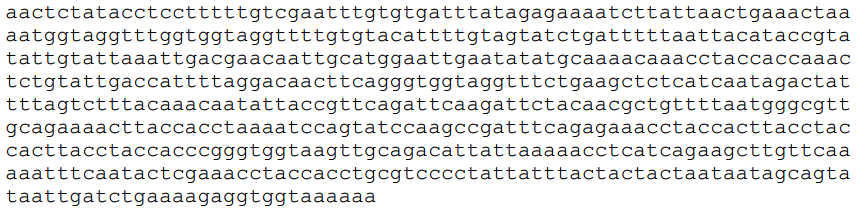
\includegraphics[width=1\textwidth]{poglavlja/1/slike/OriC_TP.png}
\caption{Prikaz \textit{oriC} regiona Thermotoga petrophila}
\end{figure} 

Možemo lako uočiti da se u ovom regionu nigde ne javljaju niske ATGATCAAG ili CTTGATCAT, iz čega zaključujemo da različite bakterije mogu koristiti različite DNKA boksove, kako bi pružile skrivenu poruku DNKA proteinu. Odnosno, za različite genome imamo različite DNKA boksove.

Najčešće reči u ovom \textit{oriC} su:  AACCTACCA, ACCTACCAC, GGTAGGTTT, TGGTAGGTT, AAACCTACC, CCTACCACC. Pomoću alata koji se zove Ori-Finder, nalazimo CCTACCACC i njegov komplement GGTGGTAGG kao potencijalne DNKA boksove naše bakterije. Ove dve niske se pojavljuju ukupno 5 puta.

\iffalse 
\begin{figure}[h]
\centering
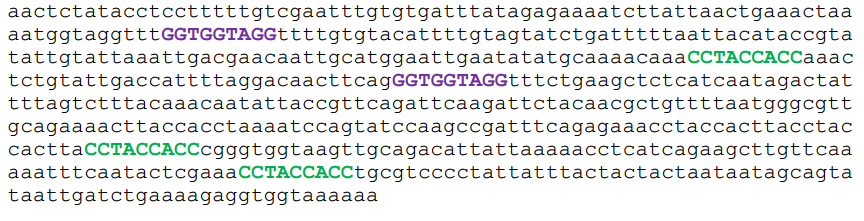
\includegraphics[width=1\textwidth]{poglavlja/1/slike/TP.png}
\caption{Prikaz CCTACCACC i njenog komplementa u \textit{oriC} regionu Thermotoga petrophila}
\end{figure}
\fi
 
Naučili smo da pronađemo skrivene poruke ako je \textit{oriC}
dat, ali ne znamo da pronađemo \textit{oriC} u genomu.

\subsection{Pronalaženje početnog regiona replikacije}

Zamislimo da pokušavamo da nađemo \textit{oriC} u novom sekvenciranom genomu bakterije. Ako bismo tražili niske poput ATGATCAAG/CTTGATCAT ili CCTACCACC/GGTGGTAGG to nam verovatno ne bi mnogo pomoglo, jer novi genom može koristiti potpuno drugačiju skrivenu poruku. Posmatrajmo, zato, drugačiji problem: umesto da tražimo grupe određenog k-grama, pokušajmo da nađemo svaki k-gram koji formira grupu u genomu. Nadajmo se da će nam lokacije ovih grupa u genomu pomoći da odredimo lokaciju \textit{oriC}-a.\\Ideja je da pomeramo prozor fiksirane dužine L kroz genom, tražeći region u kome se k-gram pojavljuje više puta uzastopno. Za L ćemo uzeti vrednost 500, koja predstavlja najčešću dužinu \textit{oriC}-a kod bakterija. \\\\
Definisali smo k-gram kao \textit{grupu}, ako se pojavljuje više puta unutar kratkog intervala u genomu. Formalno, k-gram $Pattern$ formira $(L, t)$ grupu unutar niske $Genome$ ako postoji interval genoma, dužine $L$, u kome se k-gram pojavljuje barem $t$ puta. \\\\
\begin{tcolorbox}
\textbf{Problem pronalaženja grupa.} Naći k-grame koji
formiraju grupe unutar niske karaktera.\\
\textit{Ulaz:} Niska Genome i celi brojevi k (dužina
podniske), L (dužina prozora) i t (broj podniski u
grupi).\\
\textit{Izlaz:} Svi k-grami koji formiraju (L, t)-grupe u
niski Genome.
\end{tcolorbox}

U genomu bakterije E.coli postoji 1904 različitih 9-
grama koji formiraju $(500,3)$-grupe. Koji od njih
ukazuje na početni region replikacije?

\subsubsection{Iskrivljeni dijagrami}

S obzirom na to da imamo veliku količinu statističkih podataka, pitamo se kako ih možemo upotrebiti da bismo došli do lokacije \textit{oriC}-a? U tome nam mogu pomoći \textbf{iskrivljeni dijagrami} (engl. \textit{skew diagram}). Osnovna ideja je da prođemo kroz genom i da računamo razliku između količine guanina(G) i citozina(C). Ako ova razlika raste, onda možemo pretpostaviti da se krećemo niz polulanac koji ide na desno (u nastavku samo polulanac, smer $5'\longrightarrow 3'$), a ako razlika počne da se smanjuje, onda pretpostavljamo da smo na obrnutom polulancu ($3' \longrightarrow 5'$). Zbog procesa koji se naziva deaminacija (gubljenje aminokiselina), svaki polulanac ima manjak citozina u poređenju sa guaninom, a svaki obrnuti polulanac ima manjak guanina u odnosu na citozin. 

\begin{figure}[h]
\centering
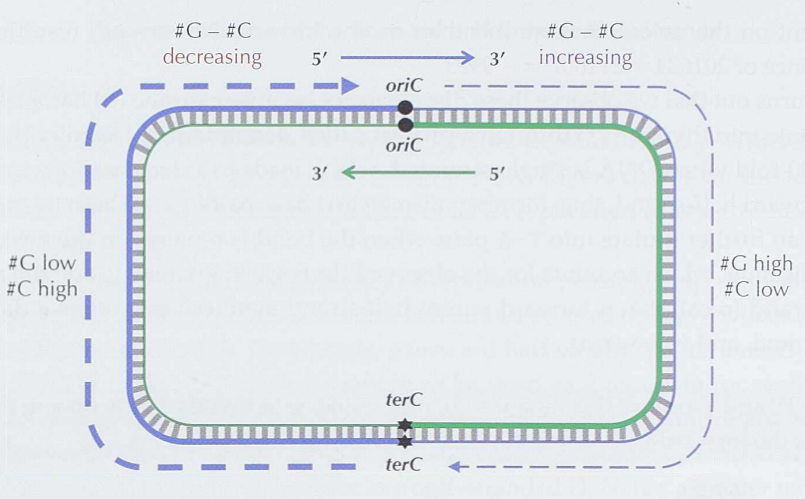
\includegraphics[width=1\textwidth]{poglavlja/1/slike/Polulanci_CG.png}
\caption{Prikaz kretanja.}
\end{figure} 

\begin{figure}[h]
\centering
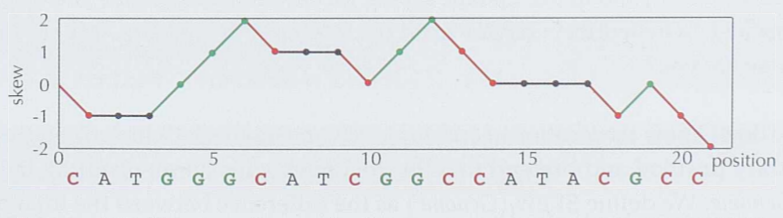
\includegraphics[width=1\textwidth]{poglavlja/1/slike/skew.png}
\caption{Iskrivljeni dijagram genoma Genome = CATGGGCATCGGCCATACGCC.}
\end{figure} 

Posmatrajmo iskrivljeni dijagram bakterije Ešerihija Koli. Lako uočavamo minimalnu vrednost skew dijagrama.

\iffalse 
\begin{figure}[h]
\centering
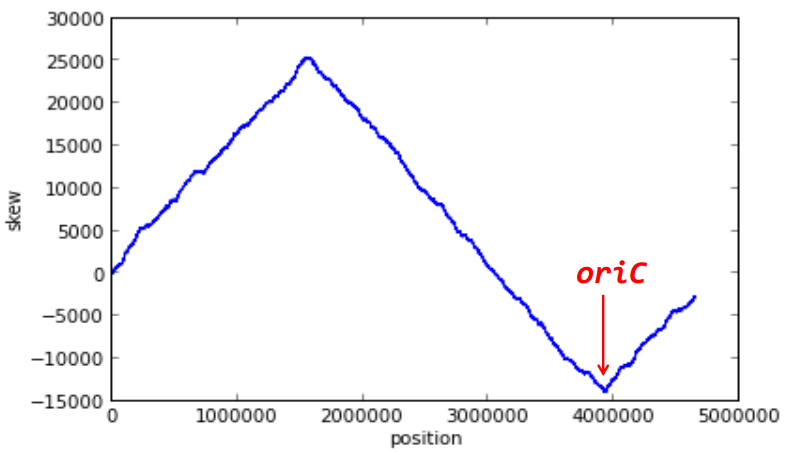
\includegraphics[width=1\textwidth]{poglavlja/1/slike/Ecoli_oriC.png}
\caption{Iskrivljeni dijagram Ešerihije koli.}
\end{figure} 
\fi 

Minimalna vrednost iz iskrivljenog dijagrama ukazuje baš na ovaj region:

\begin{figure}[H]
\centering
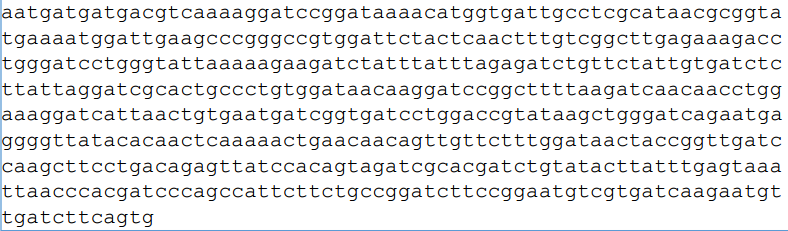
\includegraphics[width=1\textwidth]{poglavlja/1/slike/ecoli_region.png}
\caption{Region na koji pokazuje minimalna vrednost iskrivljenog dijagrama Ešerihije koli.}
\end{figure} 

Uočimo da u ovom regionu nema čestih 9-grama (koji se pojavljuju 3 ili više puta). Iz toga zaključujemo da, iako smo uspeli da nađemo \textit{oriC} bakterije Ešerihija koli, nismo uspeli da nađemo DNKA boksove. Međutim, pre nego što odustanemo od potrage, osmotrimo još jednom \textit{oriC} Vibrio colerae, kako bismo pokušali da nađemo način da izmenimo naš algoritam i uspemo da lociramo DNKA boksove u Ešerihiji koli. Veoma brzo, može se uvideti da osim tri pojavljivanja ATGATCAAG i tri pojavljivanja CTTGATCAT, \textit{oriC} Vibrio cholerae sadrži i dodatna pojavljivanja ATGATCAAC i CATGATCAT koji se razlikuju samo u jednom nukleotidu od gornjih niski. Ovo još više povećava šanse da smo naišli na prave DNKA boksove, a ima i biološkog smisla. Naime, DNKA se može vezati i za nesavršene DNKA boksove, one koji se razlikuju u nekoliko nukleotida.\\\\

\iffalse 
\begin{figure}[H]
\centering
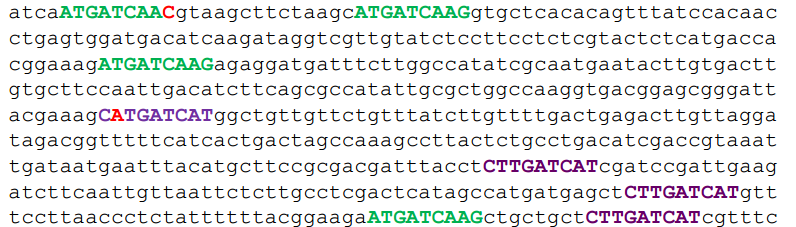
\includegraphics[width=1\textwidth]{poglavlja/1/slike/nesavrseni1.png}
\caption{Prikaz pojavljivanja nesavršenih niski nukleotida.}
\end{figure} 
\fi 

Cilj nam je da sada izmenimo algoritam čestih reči ($FrequentWords$) tako da možemo da pronađemo DNKA boksove koji su predstavljeni čestim k-gramima, sa mogućim izmenama na pojedinim nukleotidima. Ovaj problem nazvaćemo problem čestih reči sa propustima.

\begin{tcolorbox}
\textbf{Problem čestih reči sa propustima.} Pronaći najčešće k-grame sa
propustima u niski karaktera.\\
\textit{Ulaz:} Niska Text i celi brojevi k i d.\\
\textit{Izlaz:} Svi najčešći k-grami sa najviše d propusta u niski Text.
\end{tcolorbox}

Pokušajmo, još jednom, sa pronalaskom DNKA boksova kod Ešerihije koli, tako što ćemo naći najčešće 9-grame sa propustima i komplementima u regionu \textit{oriC} koji nam je predložen minimalnom vrednošću iskrivljenog dijagrama. Pokušaćemo sa malim prozorom koji ili počinje ili se završava ili je centriran na poziciji najmanje iskrivljenosti. Ovakvim izvođenjem pronalazimo TTATCCACA/TGTGGATAA kao najčešći 9-gram. Međutim, ovo nije jedini 9-gram. Za ostale 9-grame još uvek ne znamo čemu služe, ali znamo da nose skrivene informacije, da se grupišu unutar genoma i da većina njih nema veze sa replikacijom. 

\begin{figure}[H]
\caption{Prikaz pronađenih niski sa propustima i komplementima u \textit{oriC} regionu Ešerihije koli.}
\centering
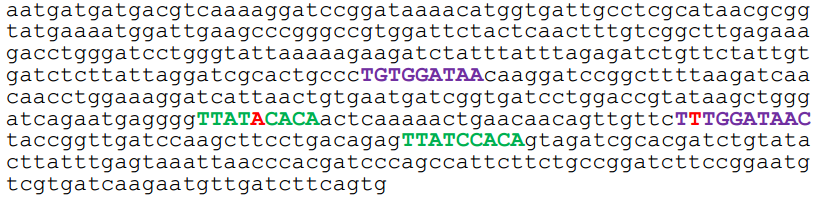
\includegraphics[width=1\textwidth]{poglavlja/1/slike/ecoli_poslednji.png}
\end{figure} 


\chapter{Koji DNK šabloni igraju ulogu molekularnog sata?}
\section{Biološki problem}

Bioritam svih živih bića kotroliše ‚‚unutrašnji časovnik'' koji još zovemo i cirkadijalni. Ljudi koji često putuju avionom na drugi kraj sveta mogu to da osete kada pokušaju da zaspe nakon promene nekoliko vremenskih zona. Kao i svaki sat, i ovaj može da se pokvari, što rezultuje genetskom bolešću pod nazivom sindrom odložene faze spavanja. Njegova osnova je na molekularnom nivou. Mnogi procesi su kontrolisani ovim časovnikom, što ilustruje slika 2.1. Kao što vidimo, postoji tačno određeno vreme u toku dana kada telo ima najnižu temperaturu, kada kreće i prestaje lučenje hormona poput melatonina (neophodnog za kvalitetan san) i slično.

\iffalse 
\begin{figure}[h]
\centering
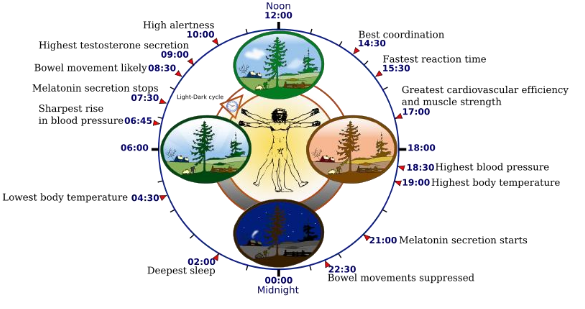
\includegraphics[width=1.1\textwidth]{poglavlja/2/slike/12cut.PNG}
\caption{Cirkadijalni ritam}
\end{figure}
\fi 

Naučnici su se pitali kako ćelije znaju kada treba da uspore ili ubrzaju proizvodnju određenih proteina. Ranih sedamdesetih, Ron Konopka i Sejmor Benzer su napravili prve korake ka rešavanju ove misterije. Do danas je otkriveno mnogo cirkadijalnih gena koji koordiniraju ponašanje stotine drugih gena. \\
\indent Kod čoveka, cirkadijalni ritam je promenljiv, tj. varira od osobe do osobe. Mi ćemo se u daljem tekstu fokusirati na biljke, jer je kod njih cirkadijalni ritam pitanje života i smrti, stoga ne sme biti promenljiv. Geni biljaka moraju znati kada sunce izlazi i zalazi kako bi znali kada treba vršiti fotosintezu, jer je ona od krucijalne važnosti za život biljke, a usko povezana sa količinom sunčeve svetlosti. Primeri specifičnih ponašanja nekih biljaka u zavisnosti od cirkadijalnog ritma dati su na slici 2.2.

\iffalse 
\begin{figure}[!htb]\centering
    \caption{Cirkadijalni ritam biljke}
   \begin{minipage}{0.5\textwidth}
     \frame{
\includegraphics[width=.7\linewidth]{poglavlja/2/slike/13-1.PNG}}
   \end{minipage}
   \begin {minipage}{0.4\textwidth}
     \frame{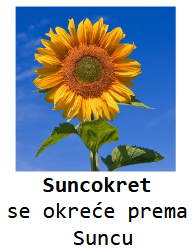
\includegraphics[width=.7\linewidth]{poglavlja/2/slike/13-2.PNG}}
   \end{minipage}
\end{figure}
\fi 

Ispostavlja se da svaka ćelija biljke čuva podatak o tome da li je dan ili noć nezavisno od drugih ćelija, kao i da su samo tri gena odgovorna za upravljanje satom. Oni kodiraju regulatorne proteine (transkripcione faktore)- to su LCY, CCA1 i TOC1. Spoljašnji faktori, kao što je količina sunčeve svetlosti, kontrolišu regulatorne gene i regulatorne proteine kako bi organizmi prilagodili svoju gensku ekspresiju, odnosno da li će se protein sintetisati u to vreme ili ne. Dakle, svaki metabolički proces je regulisan cirkadijalnim časovnikom kojim upravljaju regulatorni proteini, odlučujući kada će se koji protein u ćeliji biljke sintetisati. Regulatorni proteini upravljaju genskom ekspresijom tako što se vežu za DNK u trenucima kada je potrebno sintetisati neki protein važan za cirkadijalni ritam, kao što je prikazano na slici 2.3. Naravno, to vezivanje se ne može ostvariti bilo gde u okviru DNK, već postoje posebna mesta, kao što je prikazano na slici 2.4. Ta posebnost je neophodna iz više razloga. Regulatorni protein mora znati gde treba da se veže, a isto tako DNK mora znati kako da to protumači, odnosno, to za nju mora biti signal da je vreme započeti sintezu, kao i pružiti informaciju o kom se proteinu radi. Ta posebna mesta predstavljaju manje skupove nukleotida u DNK koji nazivamo \textbf{regulatorni motivi}. Naš zadatak je da ih pronađemo. 

\iffalse 
\begin{figure}[h]
\caption{Regulatorni proteini na delu}
\centering
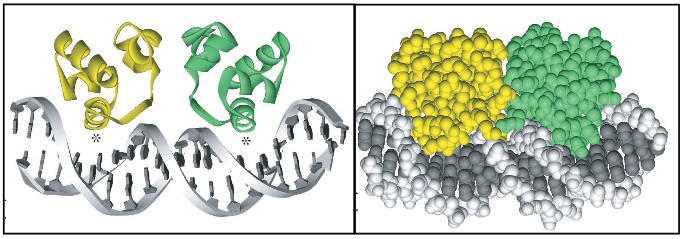
\includegraphics[width=0.55\textwidth]{poglavlja/2/slike/14.PNG}
\end{figure}
\fi 

\begin{figure}[h]
\caption{Mesta vezivanja regulatornih proteina}
\centering
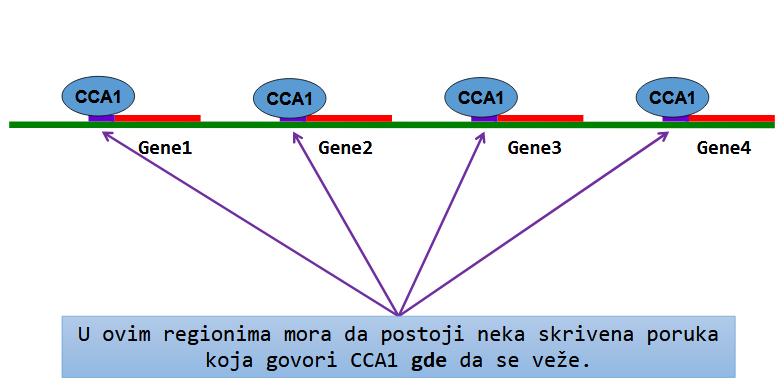
\includegraphics[width=0.7\textwidth]{poglavlja/2/slike/16.PNG}
\end{figure}


\section{Informatički problem}

Kako bismo informatički rešili problem pronalaženja regulatornih motiva u DNK, moramo predstaviti sve gorepomenute biološke pojmove na način koji bi informatičar i njegov računar mogli razumeti i obraditi. 

\begin{itemize}
    \item Iz ove tačke gledišta, DNK predstavlja nisku karaktera nad azbukom: {A, G, T, C}.
    \item Kodirajuće sekcije DNK (one koje se prepisuju i prevode u proteine) za nas će biti podniske niske DNK.
    \item Regulatorni motiv je šablon koji se pojavljuje tačno jednom u svakoj kodirajućoj sekciji DNK.
\end{itemize}

Hajde da damo u računarskom smislu korektnu definiciju problema: \\
\begin{tcolorbox}
\textbf{Informatička definicija problema nalaženja regulatornih motiva u DNK} \\
\textbf{Ulaz:} N niski koje predstavljaju kodirajuće sekvence DNK.\\
\textbf{Izlaz:} Podniska dužine k koja predstavlja regulatorni motiv (skrivenu poruku, mesto vezivanja regulatornih proteina).
\end{tcolorbox} 

Ovaj problem nas podseća na problem pronalaženja \textit{OriC}-a, koji smo rešavali svodeći ga na pronalaženje čestih reči u tekstu koristeći algoritam \textit{FrequentWords}, detaljno opisan u prethodnom poglavlju. Da bismo taj algoritam primenili ovde, neophodno je da od niza niski dobijemo konkatenacijom jednu veliku nisku, na koju ćemo primeniti ovaj algoritam. \\

Međutim, ovaj algoritam nije primenljiv ako motivi mutiraju. Možemo pokušati da primenimo algoritam \textit{FrequentWordsWithMissmatches}. To bi nas dovelo do tačnog rešenja, ali nakon previše vremena. Naime, kada smo nalazili \textit{OriC}, tražili smo uzorke dužine 9 karaktera (DnaA box je bio te dužine). U ovom slučaju, tražimo motive koji su najčešće dužine 15 karaktera, pa nam ovaj algoritam ne radi dovoljno brzo. Dakle, potrebna nam je nova ideja. 

\section{Problem ubačenog motiva}

I dalje pokušavamo da pronađemo skrivenu poruku u DNK koja kodira mesto vezivanja regulatornih proteina za DNK. Dali smo korektnu definiciju problema i, kao pravi matematičari, pokušali najpre da svedemo problem na neki drugi, koji smo već rešili. Međutim, to nas je odvelo u veliku vremensku složenost, pa samim tim i neupotrebljivost pronađenog algoritma za rešavanje. Zaključili smo da nam je potreban novi pristup, tj. da moramo probati da problem rešimo direktno - bez pomoći algoritama za \textit{OriC}. Za ovako nešto, neophodno je najpre definisati još nekoliko pojmova vezanih za šablone koje pokušavamo da pronađemo:

\begin{itemize}
    \item Mutirani šablon predstavlja šablon u kome se na nekim mestima može pojaviti mutacija, odnosno odstupanje od početne niske.
    \item $(k, d)$ motiv je k-gram koji se pojavljuje u svakoj sekvenci sa najviše $d$ razlika.
    \item Kanonski motiv predstavlja motiv koji tražimo (bez uticaja mutacija).
    \item Instance su mutirani motivi - oni koji se pojavljuju u niskama sa najviše $d$ grešaka, odnosno razlika u odnosu na kanonski motiv.
\end{itemize}

Sada, kada smo tačno i precizno definisali pojmove koji će nam igrati uloge regulatornih motiva, izmenićemo i samu definiciju problema, tj. malo promeniti scenario tako da se sve uloge lepo uklope, pazeći naravno da ne izgubimo na tačnosti definicije.

\begin{tcolorbox}
\textbf{Problem ubačenog motiva:} Pronalaženje $(k, d)$ motiva u skupu niski\\
\textbf{Ulaz:} Skup niski $Dna$ i celi brojevi $k$ (dužina motiva) i $d$ (maksimalni broj razlika).\\
\textbf{Izlaz:} Svi $(k, d)$ motivi u skupu $Dna$.
\end{tcolorbox}

Nova definicija problema izrodiće nekoliko novih ideja za njegovo rešavanje, a te ideje izrodiće nove algoritme. U daljem tekstu prikazaćemo nekoliko rešenja, uz osvrt na ideju koja nas je do njega dovela.


\subsection{Enumeracija motiva}
Početna ideja je zasnovana na gruboj sili - za svaki k-gram ćemo ispitati da li je $(k, d)$ motiv za dati skup niski. Dakle, trebalo bi generisati $4^k$ kombinacija i za svaku ispitati da li je $(k, d)$ motiv. Postavlja se pitanje da li je potrebno ispitati svih $4^k$ kandidata. 

\noindent Pogledajmo na primer sledeći skup niski:
$$\textbf{AAATTTAAATTTAAATTT}$$ 
$$\textbf{TTTAAATTTAAATTTAAA}$$
Da li ima smisla proveravati 8-gram GGAAGGAA?
Naravno da nema! Karakter G se ne pojavljuje ni u jednoj niski iz našeg skupa.
Zato sigurno ne može biti traženi $(k,d)$ motiv.
Dakle, prvo možemo izbaciti kandidate koji se ne pojavljuju ni u jednoj niski iz skupa $Dna$.
Takođe, možemo primetiti da je skup instanci jednog kandidata koje se pojavljuju u ostalim niskama (ceo skup $Dna$, bez niske u kojoj je dati kandidat podniska) prilično ograničen. Ograničenje nameće broj $d$. Dakle, jasno je da treba proveravati samo one instance koje se od kandidata razlikuju na najviše $d$ pozicija. 
Ovako redukovana pravila potrage iznedriće algoritam koji se naziva \textit{MotifEnumeration}, koji bismo u obliku pseudokoda predstavili na sledeći način:

\begin{lstlisting}
MotifEnumeration(Dna, k, d)
	for each k-mer a in Dna
		generate all possible k-mers a1 differing from a 
		by at most d mutations
    	
		for each such k-mer a1
			if a1 is a (k, d)-mer in each sequence in Dna
				output a1
\end{lstlisting}

\noindent Ovaj algoritam je suviše spor kada su $k$ i/ili $d$ veliki brojevi. Hajde da malo analiziramo složenost ovog algoritma. Možemo videti da najveću (i jedinu) komponentu složenosti čini dvostruka for-petlja, koja zavisi od broja kandidata koje pretražujemo i broja njihovih instanci. Kada su $k$ i/ili $d$ veliki brojevi, instanci ima mnogo, i pretraga ide sporo. Zbog toga, u praksi, ovaj algoritam ne pokazuje dobre rezultate za velike vrednosti $k$ i/ili $d$.
Dakle, potrebna nam je nova ideja.

\subsection{Najsličniji k-grami u parovima niski}

Videli smo da pretraga grubom silom ima veliku složenost, usled (iako redukovanog ali i dalje ogromnog) broja kandidata i njihovih instanci. Pokušali smo da redukujemo broj provera i nismo postigli mnogo. To nas dovodi do razmišljanja da ključ rešenja optimalnog algoritma ne leži u broju, već možda u redosledu. Hajde da konstruišemo ovakav primer: \\
$$ \textbf{atcgtcagAAATTTAAAGGGgtcaactg} $$
$$ \textbf{ggatcaagctAAATCTAAAGGGcttcag} $$
$$ \textbf{gatctacccaAAACTTAAAGGGgtaaac} $$
Velikim slovima predstavljen je (12,1)-motiv koji tražimo. Grubom silom pretraga bi počela na samom početku prve niske. Kako naš motiv počinje na 9. poziciji prve niske, vidimo da bi 8 puta naleteli na ćorsokak. To znači da bi se 8 velikih iteracija izvršilo uzalud. Ako bismo nekako mogli početi od devete pozicije, uštedeli bismo vreme. Ali, kako da znamo koja je tajna pozicija od koje treba krenuti? Primećujemo da se podniske atcgtcag i ggatcaag prilično razlikuju (7/8 pozicija razlike). Dakle, to sigurno ne može biti sastavni deo neke instance. Medutim, podniske AAATTTAAAGGG i AAATCTAAAGGG su prilično slične (1/12 pozicija razlike). To je svakako dobar kandidat. Ako bismo u prve dve niske pronašli kandidate sa dosta sličnosti, šanse da smo odmah pogodili $(k,d)$ motiv bi bile velike. Sve i da nismo, ovim putem ćemo obilaziti prvo verovatnije kandidate, pa bi ukupan broj pretraga sa velikom verovatnoćom bio dosta manji. Dakle, možemo probati da poredimo parove niski iz $Dna$, da uočimo dva najsličnija k-grama u dve niske iz $Dna$, od njih napravimo kanonski, i za njega proveravamo da li je $(k, d)$ motiv. Malo veći primer možete videti na slici \ref{slika: najslicniji kgrami} i probati sami da nađete ubačeni motiv.

\begin{figure}[h]
\centering
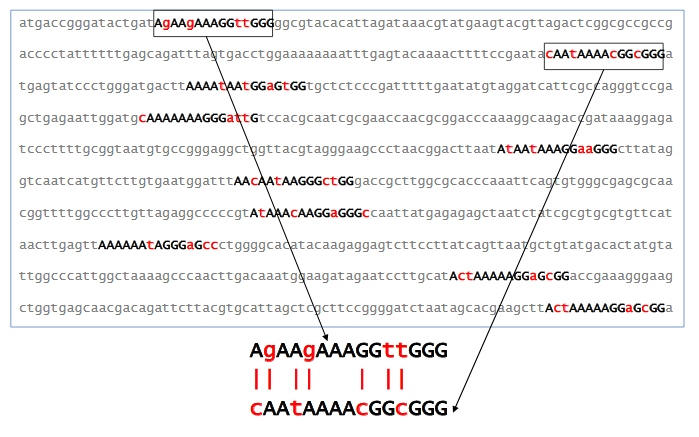
\includegraphics[width=0.9\textwidth]{poglavlja/2/slike/25.PNG}
\caption{Najsličniji k-grami u parovima niski - primer}
\label{slika: najslicniji kgrami}
\end{figure}

Zvuči predobro da bi bilo istinito? Pa možda ste i u pravu. 
Sličnost para niski je takođe određena brojem $d$. One se od kanonskog motiva mogu razlikovati na $d$ pozicija, što znači da se među sobom, mogu razlikovati na $2d$ pozicija.
Na malom izolovanom primeru, gde je bilo $d = 1$, zaista su slične niske isplivale kao dobri kandidati. Međutim, u praksi, sa (15,4)-motivima, broj dozvoljenih razlika je malo veći, čak 8. Kako izgledaju takvi parovi, prikazano je na slici \ref{slika: kgrami problem}, gde se jasno vidi koliko je to zaista mnogo i kako ove dve niske više i nisu tako slične.

\begin{figure}[h]
\centering
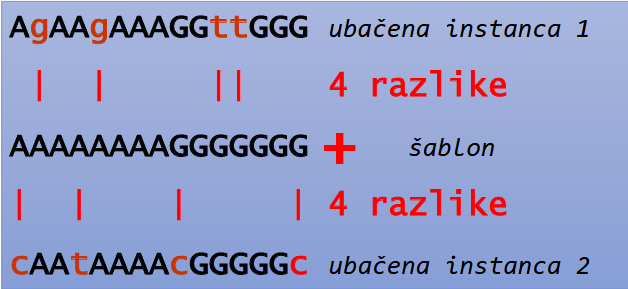
\includegraphics[width=0.7\textwidth]{poglavlja/2/slike/26.PNG}
\caption{Najsličniji k-grami u parovima niski - problem}
\label{slika: kgrami problem}
\end{figure}


Primer koji pokazuje koliko je ovo zaista loše rešenje je eksperiment rađen nad 10 slučajno generisanih niski iz $Dna$ dužine 600, sa ubačenim (15, 4) motivom. Pristupom pronalaženja parova niski iz $Dna$, pronađeno je nekoliko hiljada parova k-grama koji su se razlikovali na manje od 8 pozicija. Ovo sigurno nisu skrivene poruke, jer ih je previše. 

Da bismo ih pretražili u nekom smislenom redosledu, potrebno nam je da ih nekako rangiramo. Dakle, potreban nam je novi pristup.


\subsection{Matrice motiva}


Dosadašnje pretrage skupa $Dna$, nisu dale dobre rezultate. Pokušavali smo da ubrzamo pretragu na razne načine, ali bez puno uspeha. Možda je vreme da probamo da potpuno promenimo pristup, da mislimo izvan kutije. Pokušajmo da analiziramo jedan skup rešenja, i da malim koracima unazad dođemo do početnih uslova.

Pretpostavićemo da imamo neku kolekciju motiva i stavimo ih u matricu. Recimo da smo uradili jednom grubu pretragu i dobili neke rezultate. Da bismo olakšali komunikaciju, uvešćemo par pojmova koje ćemo koristiti u daljem tekstu.

\begin{itemize}
    \item Najpopularniji nukleotid u nekoj koloni matrice je onaj koji se pojavljuje najveći broj puta.
    \item Konsenzus niska predstavlja nisku koja se dobija nadovezivanjem najpopularnijih nukleotida iz svake kolone.
    \item Skor predstavlja broj nepopularnih simbola (onih koji nisu najpopularniji u svojoj koloni) u matrici.
\end{itemize}

Za lakše usvajanje, ilustrovani primer ovih pojmova prikazan je na slici \ref{slika: motivi skor}. Najpopularniji nukleotidi u svakoj koloni matrice motiva su napisani velikim slovima i boldovani. Oni su nadovezani u konsenzus nisku. Nepopularni simboli su napisani malim slovima, i njihov ukupan broj predstavlja skor.


\begin{figure}[h]
\centering
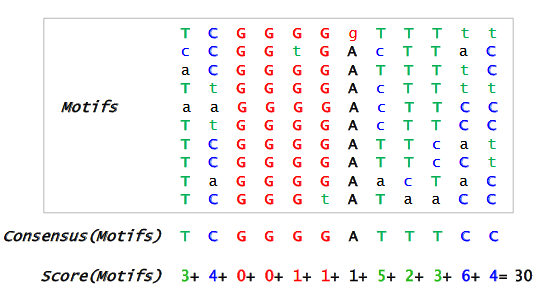
\includegraphics[width=0.9\textwidth]{poglavlja/2/slike/30.PNG}
\caption{Matrica motiva, konsenzus niska i skor}
\label{slika: motivi skor}
\end{figure}

Analizirajmo malo našu matricu rešenja. Ako bismo pretpostavili da su ovo instance nekog $(k,d)$ motiva, jasno, želeli bismo da one budu što sličnije, tj. da se razlikuju na što manje pozicija. Dakle, želimo da nam broj nepopularnih simbola bude što manji, odnosno želimo mali skor. Dakle, ako ovako postavimo problem, skor je zapravo "mera neuspeha", pa je ključ dobrog rešenja u minimizovanju ove veličine. Novi pojmovi, novi pristup i nova ideja, zahtevaju i malo drugačiju definiciju problema:

\begin{tcolorbox}
\textbf{Problem pronalaženja motiva:} Za dati skup niski iz $Dna$ naći skup k-grama (po jedan iz svake niske) sa minimalnim skorom među svim mogućim k-gramima iz datog skupa niski.\\
\textbf{Ulaz:} skup niski $Dna$ i ceo broj $k$.\\
\textbf{Izlaz:} skup k-grama $Motifs$, po jedan iz svake niske $Dna$, tako da je vrednost skora matrice $Motifs$ minimalna.
\end{tcolorbox}

Kada smo definisali problem, vreme je da krenemo da ga rešavamo.
Prvo što nam svakako pada na pamet je gruba sila. To je obično najjednostavniji algoritam, sa ne tako dobrom brzinom. Ali, ako on da zadovoljavajuću brzinu, nema potrebe komplikovati dalje, zar ne?

Dakle, krećemo redom. Uzimamo po jedan k-gram iz svake niske skupa $Dna$ i računamo skor. Tako redom obiđemo sve kombinacije k-grama, pamteći minimalni skor, i na kraju, proglasimo rešenjem onaj skup motiva sa najmanjim skorom.

Rešenje je dobro, pa hajde da pogledamo složenost. Neka je $t$ broj niski i $n$ dužina svake niske. Zaključujemo da je $(n-k+1)$ broj k-grama jedne niske, odnosno, 
$(n-k+1)^t$ broj kombinacija koje treba da proverimo. Vreme provere je konstantno (treba samo izračunati skor i ažurirati neku vrednost). Dakle, ukupna složenost je:
$(n-k+1)^t$. Eksponencijalna složenost svakako nije dobra, tako da zaključujemo da je ovaj algoritam prespor. Moramo ga nekako unaprediti.

Vratimo se na našu matricu motiva i pokušajmo da primetimo nešto što bi nam pomoglo da malo ubrzamo stvari. Pogledajmo primer dat na slici \ref{slika: motivi detaljnije}.

\begin{figure}[h]
\centering
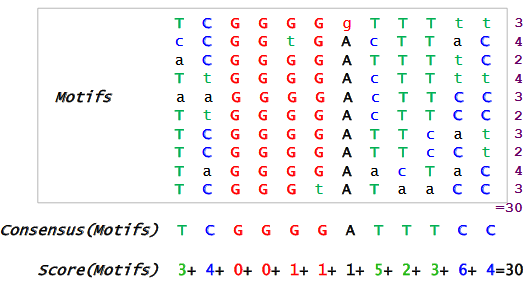
\includegraphics[width=0.9\textwidth]{poglavlja/2/slike/32.PNG}
\caption{Matrica motiva, konsenzus niska i skor - detaljnije}
\label{slika: motivi detaljnije}
\end{figure}


Izračunali smo skor po vrstama i primetili da je isti kao skor po kolonama. Da li je to slučajnost? Ispostavlja se da nije. Suština veličine skor leži u tome da broji nepopularne simbole. Nije važno kako ih prebrajamo, ako su svi na broju. 
Pojam brojanja definisaćemo na malo formalniji način. Definisaćemo veličinu koja se zove Hamingonovo rastojanje.

Hamingovo rastojanje između dve niske istih dužina predstavlja broj pozicija na kojima se one razlikuju. Npr. Hamingonovo rastojanje niski AACCTTGG i ATCCATGG je 2. Kada imamo Hamingovo rastojanje, možemo reći da je skor po kolonama suma Hamingovih rastojanja k-grama iz matrice od konsenzus niske. 


Vreme je da pokušamo da unapredimo naš algoritam. Želimo nekako da nađemo način da uradimo suprotno - da od konsenzus niske i niza $Dna$ dobijemo matricu $Motifs$. 
Koristićemo sledeće osobine koje smo primetili na matrici $Motifs$:
\begin{enumerate}
    \item Kako skor predstavlja sumu rastojanja od k-grama iz matrice do konsenzus niske, minimalni skor predstavlja minimizovanu sumu tih rastojanja.
    \item Kako je skor po kolononama i vrstama isti, možemo rastojanje računati i po vrstama. 
    Tako dolazimo do reforomulacije našeg problema, tj. njegovog ekvivalenta koji koristi naša nova zapažanja.
\end{enumerate}

Iskoristićemo ove osobine kako bismo još jednom predefinisali naš problem tako da odražava sliku iz novog pristupa.

\begin{tcolorbox}
\textbf{Problem pronalaženja motiva - reformulacija:} Naći k-gram $Pattern$ i skup k-grama $Motifs$ iz skupa niski $Dna$ koji minimizuju rastojanje između svih mogućim k-grama $Pattern$ i svih mogućih skupova k-grama $Motifs$.\\
\textbf{Ulaz:} skup niski iz $Dna$ i ceo broj $k$.\\
\textbf{Izlaz:} k-gram $Pattern$ i skup k-grama $Motifs$ iz skupa niski $Dna$ koji minimizuju $d(Pattern, Motifs)$.
\end{tcolorbox}

\noindent Ovo je ekvivalentno našem prethodnom problemu jer smo primetili da $d(Pattern, Motifs)$ predstavlja skor ukoliko je $Pattern$ konsenzus niska. Postavlja se pitanje da li smo ovim otežali naš problem. Ispostaviće se da nismo, jer ne moramo ispitivati sve skupove k-grama $Motifs$, već je dovoljno da iskoristimo problem niske medijane koji ispituje sve k-grame $Pattern$. 

\subsection{Problem niske medijane}
Prethodnom definicijom problema, nameće se zaključak da je sledeći prirodni korak proći kroz sve kombinacije skupa k-grama $Motifs$ i k-grama $Pattern$, kako bismo našli kombinaciju sa najmanjim rastojanjem. Međutim, videli smo i da algoritmi zasnovani na gruboj sili, tj. iscrpnoj pretrazi kombinacija u potrazi za pravom, vode ka ogromnoj složenosti i lošoj praktičnoj primeni. 

Zato ćemo ovaj put preskočiti taj korak i odmah krenuti da modifikujemo algoritam tako da dobijemo manju složenost. Primetićemo da imamo dve dimenzije pretrage (računarski bi to bile dve ugnježdene for petlje). Jedna je po svim k-gramima $Pattern$ a druga po skupovima $Motifs$. Jasno je da bi se složenost prepolovila (tj. korenovala) ako bismo imali samo jednu dimenziju. Zvuči neverovatno, ali je moguće, ako primetimo da nam unutrašnja for petlja nije potrebna, jer možemo uzeti cele niske umesto motiva. Tačnije, želimo da računamo rastojanje jednog k-grama od celog skupa $Dna$. Računanjem rastojanja od samih niski iz $Dna$ umesto od njihovih podniski dužine $k$, štedimo dosta vremena, a postižemo isti efekat. Međutim, da bismo to učinili, najpre moramo definisati nekoliko pojmova, na prvom mestu jer još uvek nismo rekli kako se računa rastojanje sem ako imamo dve niske i to iste dužine. Dakle, definisaćemo najpre sledeće pojmove: 

\begin{itemize}
    \item Hamingovo rastojanje izmedu dve niske različitih dužina predstavlja minimum Hamingovih rastojanja između kraće niske i svih podniski duže niske odgovarajuće dužine.
    \item Definišemo rastojanje između k-grama i skupa (dužih) niski kao sumu rastojanja između tog k-grama i svih niski iz skupa.
    \item Niska medijana za skup niski $Dna$ predstavlja onaj k-gram koji minimizuje rastojanje izmedu tog k-grama i skupa $Dna$ - $d(k-gram, Dna)$.
\end{itemize}

Novi pojmovi i nova ideja, prirodno vode i do nove definicije problema. Moramo dobro definisati problem koji rešavamo ako želimo da nas to dovede do dobrog algoritma za njegovo rešavanje.

\begin{tcolorbox}
\textbf{Problem niske medijane:} pronaći nisku medijanu.\\
\textbf{Ulaz:} skup niski $Dna$.\\
\textbf{Izlaz:} k-gram $k-mer$ koji minimuzuje rastojanje d($k-mer$, $Dna$).
\end{tcolorbox}

Sada imamo sav potreban alat da rešimo problem. Eliminišući jednu dimenziju, pretragu ćemo vršiti samo po svim mogućim kombinacijama k-grama $Pattern$ (njih $4^k$) i kao rezultat vratiti onaj k-gram koji ima najmanje ratojanje od skupa $Dna$. Ovaj algoritam se naziva \textit{MedianString} i prikazan je sledećim pseudokodom:

\begin{lstlisting}[escapeinside={(*}{*)}]
MedianString(Dna, k)
	best-k-mer (*$ \leftarrow $*) AAA...AA
    for each k-mer from AAA...AA to TTT...TT
        if d(k-mer, Dna) < d(best-k-mer, Dna)
            best-k-mer (*$ \leftarrow $*) k-mer
    return best-k-mer
\end{lstlisting}

Hajde da analiziramo složenost i vidimo da li smo zaista napredovali. Neka je $t$ dužina niza $Dna$ i $n$ dužina niske iz $Dna$. Tada nam je za izračunavanje rastojanja između jednog k-grama i jedne niske iz skupa $Dna$ potrebno $k \cdot (n-k+1)$ poređenja. Kako imamo $t$ niski, za izračunavanje rastojanja k-grama od skupa potrebno nam je $t \cdot k \cdot (n-k+1)$, odnosno približno $t \cdot k \cdot n$, jer je $n$ daleko veće od $k$ pa čini primarnu komponentu složenosti u $(n-k+1)$. Ceo taj postupak moramo izvršiti za svaki k-gram, odnosno $4^k$ puta, pa imamo, dakle, da ukupna složenost algoritma iznosi: $4^k \cdot n \cdot t \cdot k$. Primećujemo da je ovo dobar napredak u odnosu na $n^t \cdot k \cdot t$, ali i dalje imamo eksponencijalnu složenost. Dakle, iako je \textit{MedianString} algoritam mnogo brži od grube sile, za velike $k$ je i dalje prespor. 

\subsection{Probabilistički pristup}

\subsubsection{Uopšteno o pristupu}

Analizirali smo nekoliko determinističkih algoritama i videli da, iako uvek daju tačno rešenje, troše preveliku količinu vremena. Čak i najbolji među njima, \textit{MedianString}, imao je eksponencijalnu složenost. To nas navodi na razmišljanje da je možda ponovo došlo vreme da uradimo veliki zaokret u pristupu samom problemu i pokušamo da nađemo kompromis između tačnosti i utroška vremena. Algoritmi koji ovo omogućavaju se nazivaju probabilistički algoritmi. Oni daju tačno rešenje sa određenom verovatnoćom, ali za dosta manje vremena, i oni su naša sledeća stanica u potrazi za ubačenim motivima. Kao i svaki put kada menjamo pristup, upoznaćemo se najpre sa nekoliko osnovnih pojmova:
 
\begin{itemize}
    \item \textit{Count} matrica neke matrice motiva prikazuje koliko se puta koji nukleotid ponavlja u svakoj koloni matrice motiva.
    \item Profilna matrica neke matrice motiva prikazuje učestalost pojavljivanja nukleotida u svakoj koloni matrice motiva.
\end{itemize}

Ilustrovani primer ovih pojmova prikazan je na slici 2.9.

\begin{figure}[h]
\caption{\textit{Count} i profilna matrica}
\centering
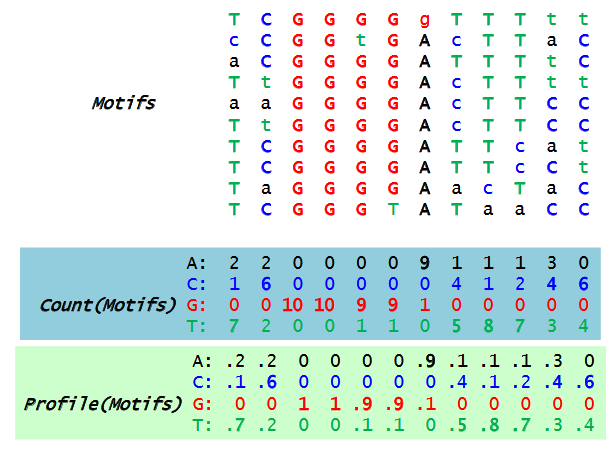
\includegraphics[width=0.9\textwidth]{poglavlja/2/slike/56.PNG}
\end{figure}

Osnovna ideja ovog pristupa može se ilustrovati bacanjem $k$ četvorostranih kockica sa otežanim stranama. Svaka kockica pretstavlja jednu poziciju u motivu dužine $k$, i na stranama ima simbole A, C, T i G. Strane kockica su otežane, tako da svaka strana pada sa onom verovatnoćom koja je zapisana u profilnoj matrici, u preseku kolone rednog broja pozicije u motivu i reda karaktera koji je na toj strani kockice. Na primer, ukoliko imamo profilnu matricu kao na slici 2.10, bacali bismo 6 četvorostranih kockica, gde bi recimo druga kockica bila otežana tako da simbol A pada sa verovatnoćom 7/8, simbol C sa verovatnoćom 0, simbol T sa verovatnoćom 1/8 i simbol G sa verovatnoćom 0. Naravno da u praksi ne možemo imati verovatnoću nula, ali sa našim zamišljenim kockicama, to je legitimna situacija. Zašto ovo nije dobro i kako se to popravlja, diskutovaćemo malo kasnije. 

Neka su redom pali karakteri: A, T, A, C, A i G. Verovatnoću podniske koju oni čine možemo izračunati na osnovu profilne matrice, pretpostavljajući da su bacanja nezavisni događaji. Dakle, pročitaćemo iz profilne matrice verovatnoću karaktera A na prvoj poziciji (1/2), verovatnoću karaktera T na drugoj (1/8), ... , i pomnožićemo sve te vrednosti. Proizvod verovatnoća iznosi 0.001602.

\begin{figure}[h]
\caption{Računanje verovatnoće k-grama}
\centering
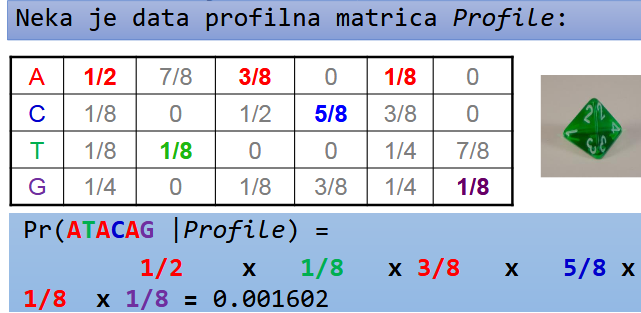
\includegraphics[width=0.5\textwidth]{poglavlja/2/slike/61.PNG}
\end{figure}

 Ako se setimo kako smo definisali matricu motiva, konsenzus nisku i profilnu matricu, lako možemo zaključiti da je ova verovatnoća zapravo verovatnoća da je niska ATACAG konsenzus niska. Sada nam same kockice više nisu potrebne, već možemo uzeti realne k-grame iz niski skupa $Dna$ i za njih računati. Na primer, za nisku CTATAAACCTTACAT iz nekog skupa $Dna$, možemo izračunati verovatnoće svih njenih podniski dužine 6 (rezultate možete videti na slici 2.11) i potražiti onaj sa najvećom verovatnoćom (u primeru sa slike 2.11 to je AAACCT). On je svakako dobar kandidat za ubačeni motiv. U ovome leži sama suština svih probabilističkih algoritama za traženje ubačenih motiva.

\begin{figure}[h]
\caption{Primer: najverovatniji 6-gram}
\centering
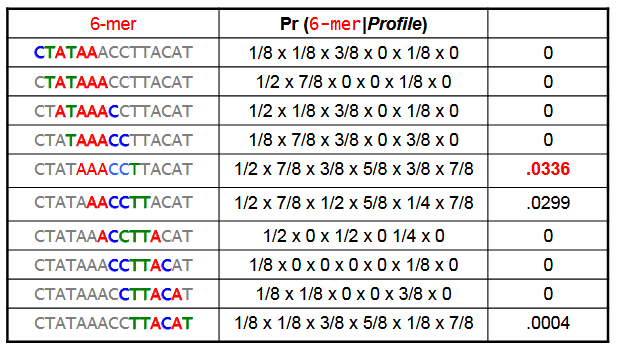
\includegraphics[width=0.8\textwidth]{poglavlja/2/slike/63-2.PNG}
\end{figure}

U daljem tekstu, predstavićemo nekoliko probabilističkih algoritama za rešavanje problema ubačenih motiva. Opisaćemo same algoritme, ali i diskutovati o njihovim dobrim i lošim stranama.

\noindent \textbf{Važna napomena}: Kao što smo već napomenuli, cenu malog vremena ovi algoritmi plaćaju tačnošću. Dakle, rešenje može malo odstupati od traženog. Zbog toga, za postizanje najbolje tačnosti, probabilističke algoritme treba pokretati više puta i uzeti najbolji rezultat.

\subsubsection{Algoritam \textit{Greedy motif search}}
Prvi algoritam koji ćemo predstaviti je pohlepni algoritam. Kao ulaz, on prima skup niski $Dna$, broj njegovih elemenata $t$ i dužinu ubačenog šablona $k$, a kao izlaz daje matricu ubačenih motiva $BestMotifs$. Suština algoritma leži u njegovom imenu: grabi k-mere iz jedne niske redom, na osnovu svakog od njih nađi najbolju matricu u koju se on uklapa, i uzmi onu koja ima najmanji skor.
Na početku $BestMotifs$ se inicijalizuje na $t$ podniski dužine $k$, od kojih svaka predstavlja prvih $k$ karakera jedne niske iz skupa $Dna$. Iterira se kroz prvu nisku skupa $Dna$, i iteracija ima onoliko koliko ima podniski dužine $k$ u njoj. U svakoj iteraciji, računa se po jedna matrica motiva. 

Građenje te matrice je jedan vid pohlepe ovog algoritma. Grabimo već izračunate vrednosti, kako bismo što bolje odredili sledeće. Prvi red čini tekuća podniska iteracije (podniska prve niske skupa $Dna$ koja počinje od karaktera na poziciji rednog broja iteracije). Za svaki sledeći red se pravi profilna matrica prethodno izračunatih redova i na osnovu nje računa najverovatnija podniska iz one niske skupa $Dna$, koja ima redni broj isti kao redni broj reda matrice koji računamo. Dakle, svaki sledeći motiv u matrici se sve lepše poklapa sa ostatkom matrice. Sledeći korak u iteraciji je da izračunamo skor i ako je manji, da ažuriramo vrednost $BestMotifs$. Dakle, ona matrica koja ima najmanji skor je tražena matrica $BestMotifs$. Sam algoritam ilustrovan je sledećim pseudokodom:


\begin{lstlisting}[escapeinside={(*}{*)}]
GreedyMotifSearch(Dna, k, t)
  BestMotifs (*$ \leftarrow $*) motif matrix formed by first k-mers in each string from Dna
  for each k-mer Motif in the first string from Dna
      Motif(*$_1 \leftarrow $*) Motif
      for i = 2 to t
        form Profile from motifs Motif(*$_1$*), ..., Motif(*$_{i-1}$*)
        Motif(*$_i  \leftarrow $*) Profile - most probable k-mer in the i-th string in Dna
      Motifs (*$ \leftarrow $*) (Motif(*$_1$*), ..., Motif(*$_t$*))
	  if Score(Motifs) < Score(BestMotifs)
        BestMotifs (*$ \leftarrow $*) Motifs
  return BestMotifs
\end{lstlisting}

\textit{GreedyMotifSearch} je brži od \textit{Median string} algoritma. Povoljan je i za veće $k$, ali cena toga je manja tačnost. Tačnost se može poboljšati primenom Laplasovog pravila, o kojem će biti nešto više reči malo kasnije.

\subsubsection{\textit{Randomized motif search}}
Posmatrajući algoritam \textit{GreedyMofifSearch}, možemo primetiti da nismo postigli pun potencijal po pitanju prelaska na probabilistički pristup. Broj iteracija je i dalje fiksan (zavisi isključivo od dužine niski iz skupa $Dna$ i dužine ubačenog motiva), a i sam njihov redosled je nametnut deterministički. Kako uvek krećemo od istog skupa motiva, i pratimo iste utabane korake, pokretanjem ovog algoritma više puta nećemo poboljšati ni tačnost ni vreme konvergencije. 

Hajde da pokušamo da potpuno izbacimo determinizam iz priče i da pustimo da izgled same niske $Dna$ i zakon verovatnoće igraju glavne uloge u konvergenciji algoritma. Prva ideja o poboljšanju probabilizma bi mogla biti vezana za sam početak algoritma. Hajde da umesto kretanja od početnih pozicija, krećemo od nekih nasumično odabranih. To sasvim sigurno donosi malo probabilizma u našu priču. Međutim, i dalje imamo iteriranje po jednoj od niski, što fiksira i broj iteracija i njihov redosled. To je ono što nam najviše i smeta. 

Na početku sekcije o probabilističkim algoritmima, naučili smo da pravimo profilnu matricu od matrice motiva, a u algoritmu \textit{GreedyMofifSearch} smo videli da je moguće i obrnuto. To je dobra ideja za osnovu iteracije. Od matrice motiva bismo mogli praviti profilnu matricu, a od profilne matrice ponovo matricu motiva. Ponavljanjem tog postupka, mogli bismo iterirati bez potrebe da se vezujemo za bilo kakav redosled podniski u nekoj od niski iz $Dna$. Ostalo je još da razmislimo kako bismo znali kada da stanemo. 

Pretpostavljajući da krećemo od neke nasumične matrice motiva sa lošim, tj. velikim skorom, pretpostavljajući da se krećemo ka dobrom rešenju koje ima mali skor, kao i da to činimo postepeno gradeći sve bolja, tj. verovatnija rešenja pomoću profilnih matrica, prirodno je da pomislimo da će se skor smanjivati iz iteracije u iteraciju. Dakle, iteriraćemo dokle god nam se skor smanjuje.

Ova ideja je zapravo osnova algoritma \textit{RandomizedMotifSearch}. Njegova suština leži u tome da u velikom broju iteracija ažuriramo matricu motiva i profilnu matricu tako da dobijamo sve verovatniji skup motiva, zaustavljajući se kada postignemo najniži skor. Ovaj algoritam je ilustrovan sledećim pseudokodom:

\begin{lstlisting}[escapeinside={(*}{*)}]
RandomizedMotifSearch(Dna, k, t)
  randomly select k-mers Motifs = (Motif(*$_1$*), ..., Motif(*$_t$*)) in each string from Dna
  bestMotifs (*$\leftarrow$*) Motifs
  while forever
    Profile (*$\leftarrow$*) Profile(Motifs)
    Motifs (*$\leftarrow$*) Motifs(Profile, Dna)
    if Score(Motifs) < Score(bestMotifs)
      bestMotifs (*$\leftarrow$*) Motifs
    else 
      return bestMotifs
\end{lstlisting}

Radi lakšeg razumevanja, hajde da ilustrujemo rad ovog algoritma na jednom primeru. Jedan takav, dosta uprošćen primer možemo videti na slici \ref{slika: randomized}. Prikazan je algoritam \textit{RandomizedMotifSearch} koji konvergira u jednoj iteraciji.

Neka je dat skup $Dna$ od 5 niski dužine 10 karaktera, sa ubačenim (4,1) motivom. Na slici \ref{slika: randomized} u gornjem levom uglu, prikazan je skup $Dna$, tako što su velikim slovima ispisani karakteri instanci ubacenog motiva: ACCT, ATGT, GCGT, ACGA i AGGT, crnom bojom označene mutacije na motivima, a plavom nemutirani karakteri motiva. 

Prvi korak jeste određivanje početne vrednosti matrice \textit{Motifs}. Odabraćemo slučajno 5 pozicija (u opsegu od 1 do 7) na kojima će početi 4-grami kojima ćemo inicijalizovati matricu \textit{Motifs}, i neka su to pozicije 7, 5, 1, 2 i 7. 4-grami koji počinju na ovim pozicijama: taac, GTct, ccgG, acta i AGGT, čine početnu matricu \textit{Motifs}. Sledeći korak jeste izgradnja profilne matrice na osnovu matrice \textit{Motifs}. Prebrojavanjem svakog karaktera u svakoj koloni matrice \textit{Motifs} možemo odrediti \textit{count} matricu, a zatim deljenjem svakog broja iz \textit{count} matrice sa brojem niski, tj. 5 u našem primeru, dobijamo profilnu matricu. 

Sada kada imamo profilnu matricu, možemo izračunati nove najverovatnije motive u niskama iz $Dna$, i ažurirati matricu \textit{Motifs}. Postupak računanja matrice motiva prikazan je na slici 2.12 u središnjem delu. Za svaku nisku iz skupa $Dna$, odredićemo verovatnoće svih njenih podniski, na osnovu profilne matrice, i iz svake niske odabrati po jednu koja ima najveću verovatnoću (na slici su prikazane ljubičastom bojom). 

Sledeći korak bi bio da ponovo napravimo profilnu matricu itd. Međutim, u našem primeru, vidimo da je to kraj. Dobili smo traženo rešenje. Treba napomenuti da je ovo veštački kreiran primer i da je u praksi broj iteracija dosta veći.

\begin{figure}[h]
\centering
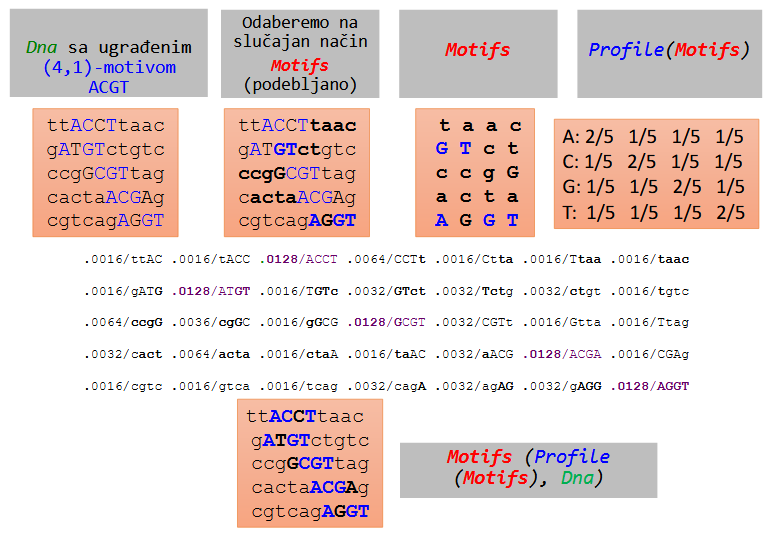
\includegraphics[width=0.8\textwidth]{poglavlja/2/slike/69.PNG}
\caption{Primer rada algoritma \textit{RandomizedMotifSearch}}
\label{slika: randomized}
\end{figure}


Velika prednost ovog algoritma je u nasumičnom izboru početnog skupa motiva, što nam omogućava da ga pokrećemo iznova i izaberemo najbolje rešenje.

\subsubsection{Gibsovo sempliranje}
Algoritam \textit{RandomizedMotifSearch} je dobar i efikasan, ali ima jednu malu manu. Matrica motiva se potpuno menja iz iteracije u iteraciju, što može dovesti do toga da se izmene i neki dobro izračunati redovi. To svakako ne želimo. Ako bismo u svakoj iteraciji menjali samo po jedan motiv iz matrice, tj. posle manjih izmena pravili novu profilnu matricu i proveravali skor, mogli bismo bolje da kontrolišemo to kvarenje već nameštenih motiva. Ova modifikacija algoritma \textit{RandomizedMotifSearch} se naziva Gibsovo sempliranje. Na prvi pogled deluje kao da povećava broj iteracija i usporava konvergenciju, ali to što su promene manje, nikako ne znači da su manje i efikasne. Ako idemo pravo sitnijim koracima, stižemo brže i lakše na cilj, nego ako krupnim koracima idemo levo-desno. 
Osnovna razlika Gibsovog sempliranja u odnosu na algoritam \textit{RandomizedMotifSearch} se nalazi u sadržaju iterativnog koraka. Umesto da od cele matrice motiva pravimo profilnu matricu i na osnovu nje ažuriramo celu matricu motiva, sada ćemo nasumično odabrati jedan motiv koji ćemo izbaciti, profilnu matricu praviti od ostatka matrice, a ažuriranje matrice motiva vršiti samo nad izbačenim redom u matrici. Postupak kreiranja same profilne matrice i ažuriranja motiva je potpuno isti kao u algoritmu \textit{RandomizedMotifSearch}. Umesto pseudokodom, ovaj put ćemo algoritam prikazati u koracima:

\begin{enumerate}
    \item Formirati \textit{Motifs} izborom jednog k-grama iz svake sekvence \textbf{na slučajan način}
    \item \textbf{Na slučajan način} odabrati jedan od k-grama i ukloniti ga iz \textit{Motifs} ; označimo sekvencu kojoj taj k-gram pripada sa \textit{RemovedSequence}
    \item Kreirati profilnu matricu \textit{Profile} od preostalih k-grama u \textit{Motifs}
    \item Za svaki k-gram iz \textit{RemovedSequence}, izračunati $Pr(k-mer|Profile)$ ; na taj način dobijamo $n-k+1$ verovatnoća: $p_1, p_2, ..., p_{n-k+1}$
    \item \textbf{Bacimo kockicu} sa $n-k+1$ strana kod koje je verovatnoća da će pasti na i-tu stranu proporcionalna verovatnoći $p_i$
    \item Odredimo k-gram iz sekvence \textit{RemovedSequence} kao onaj koji ima najveću verovatnoću i dodamo ga u \textit{Motifs}
    \item Ponavljamo korake 2-6
\end{enumerate}

Radi lakšeg razumevanja, prikazaćemo i ovaj algoritam na istom primeru kao i \textit{RandomizedMotifSearch}. Skica rada algoritma je prikazana na slici 2.13.

Neka je ponovo dat isti skup $Dna$ od 5 niski dužine 10 karaktera, sa ubačenim (4,1) motivom. Na slici \ref{slika: gibs} u gornjem levom uglu, prikazan je skup $Dna$, tako što su velikim slovima ispisani karakteri instanci ubačenog motiva: ACCT, ATGT, GCGT, ACGA i AGGT, crnom bojom označene mutacije na motivima, a plavom nemutirani karakteri motiva. Prvi korak je isti kao i u algoritmu \textit{RandomizedMotifSearch}: određivanje početne vrednosti matrice \textit{Motifs}. Odabraćemo slučajno 5 pozicija (u opsegu od 1 do 7) na kojima će početi 4-grami kojima ćemo inicijalizovati matricu \textit{Motifs}, i neka su to pozicije 7, 5, 1, 2 i 7. 4-grami koji počinju na ovim pozicijama: taac, GTct, ccgG, acta i AGGT, čine početnu matricu \textit{Motifs}. 

Sledeći korak jeste izbacivanje jednog motiva. Nasumičnim izborom jednog broja iz opsega (1,5), odredili smo motiv iz reda 3 da bude izbačen. Matrica \textit{Motifs} sada izgleda kao na slici \ref{slika: gibs} u gornjem desnom uglu. Naredni korak je izgradnja profilne matrice na osnovu matrice \textit{Motifs}. Ovaj postupak je takođe isti kao u algoritmu \textit{RandomizedMotifSearch}, samo je skup nad kojim radimo za jedan 4-gram manji. Prebrojavanjem svakog karaktera u svakoj koloni matrice \textit{Motifs} možemo odrediti \textit{count} matricu (slika \ref{slika: gibs} , centar-desno), a zatim deljenjem svakog broja iz \textit{count} matrice sa brojem motiva, tj. 4 u našem primeru, dobijamo profilnu matricu. 

Sada kada imamo profilnu matricu, možemo izračunati novi najverovatniji motiv u trećoj niski iz $Dna$, i ponovo popuniti treći red u matrici \textit{Motifs}. Vidimo da je podniska GCGT jedina sa pozitivnom verovatnoćom, pa samim tim i najvećom, tako da njome popunjavamo treći red matrice \textit{Motifs}. Sledeći korak bi bio da ponovo izbacimo nasumično odabrani motiv, napravimo profilnu matricu itd. Iterirali bismo sve dok skor ne prestane da se smanjuje. 


\begin{figure}[h]
\centering
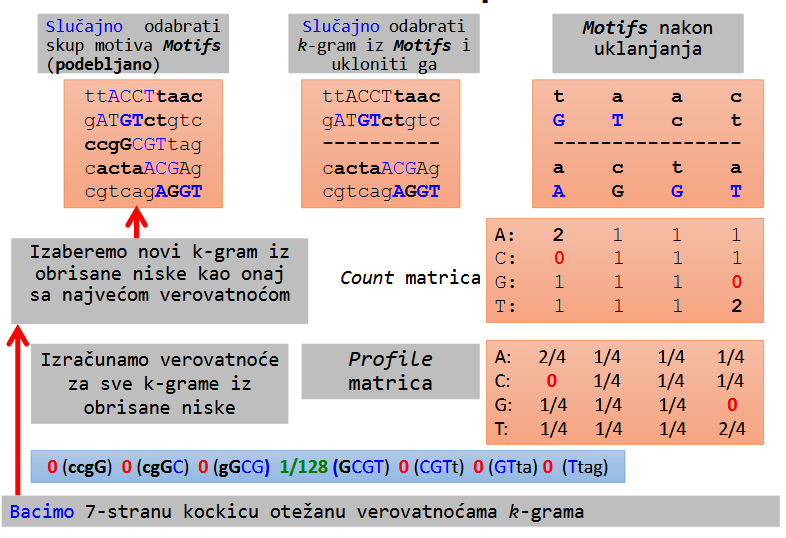
\includegraphics[width=0.8\textwidth]{poglavlja/2/slike/73.PNG}
\caption{Primer rada algoritma Gibsovo sempliranje}
\label{slika: gibs}
\end{figure}

Međutim, sada ćemo se ovde zaustaviti kako bismo primetili nešto mnogo važno. Kada smo računali verovatnoće podniski kandidata za zamenu trećeg motiva, dobili smo samo jednu ne-nula vrednost od 7. To nije dobro. Jedna nula u profilnoj matrici može anulirati verovatnoće koje su sve do množenja sa njom bile prilično velike. Zbog toga one nisu baš poželjne. Ako zastanemo malo i razmislimo, shvatićemo da nisu previše ni realne, tj. da ne odražavaju realnu verovatnoću, već da su u velikom broju slučajeva uzrokovane malim obimom skupa nad kojim računamo. Zbog toga, modifikicija nula u profilnoj matrici predstavlja vrlo dobru i poželjnu modifikaciju ovog algoritma, a ta modifikacija se sprovodi korišćenjem Laplasovog pravila.

Mala napomena: Setimo se da smo već pominjali Laplasovo pravilo kao dobro poboljšanje i \textit{GreedyMofifSearch} i \textit{RandomizedMotifSearch} algoritama. Zapravo, ovo je korisna modifikacija svakog algoritma koji se zasniva na računanju profilne matrice i korišćenju njenih vrednosti.

Pre nego pređemo na modifikaciju, naglasićemo još da se prednost Gibsovog algoritma ogleda u najmanjem skoru, kao i to da je mana ovog algoritma zaglavljivanje u lokalnom minimumu usled pretrage ograničenog skupa rešenja. 

\subsubsection{Laplasovo pravilo kao poboljšanje Gibsovog semplera}

Davne 1650. godine, Oliver Kromvel je napisao:
"Molim Vas, tako Vam Hrista, mislite da je moguće da grešite". 
Ovu izjavu, je uobličio Denis Lindli i nazvao Kromvelovo pravilo:
"Treba da ostavimo malu mogućnost da Sunce sutra neće izaći".
Nešto novija replika bi se mogla naći u seriji Smolvil i rečima Leksa Lutora: "Uvek ostavljam malu mogućnost da nisam u pravu. Tako me ništa ne može iznenaditi."
Suština Kromvelog pravila leži u tome da, ukoliko potpuno odbacimo mogućnost nekog događaja, sasvim sigurno ostavljamo mogućnost pogreške. Zbog toga, treba izbegavati verovatnoće 0 i 1.

Za poboljšanje Gibsovog semplera (zapravo se može primeniti na bilo koji algoritam koji računa profilnu matricu), izvršićemo malu modifikaciju algoritma primenom Laplasovog pravila. Primenjujemo Laplasovo a ne Kromvolevo pravilo, samo iz razloga notacije i matematičkog zapisa. Laplasovo pravilo je samo preciznija (matematička) formulacija Kromvelovog pravila, sa istom suštinom. 

\begin{tcolorbox}
\textbf{Laplasovo pravilo:} U malim skupovima podataka uvek postoji šansa da se događaj koji je moguć ne desi. Slučajni algoritmi uvode pseudovrednosti koje povećavaju verovatnoće retkih događaja i eliminišu frekvencije jednake nuli zabeležene na osnovu iskustva.
\end{tcolorbox}

\indent Suština Laplasovog pravila leži u tome da, ukoliko znamo da se događaj nekada u prošlosti desio, on ne može imati verovatnoću nula. Stoga u računanje, pored vrednosti dobijenih u našem eksperimentu, ubacujemo i dve pseudovrednosti: događaj se desio i događaj se nije desio. \\

\noindent Računanje uslovne verovatnoće bez primene Laplasovog pravila bi bilo:
\begin{tcolorbox}
Ako su $X_1, ..., X_{n+1}$ uslovno nezavisne slucajne logičke promenljive (neuspeh 0, uspeh 1), tada: $Pr(X_{n+1}=1|X_1+...+X_n=s)=s/n$
\end{tcolorbox}

\noindent Računanje uslovne verovatnoće sa primenom Laplasovog pravila bi bilo:
\begin{tcolorbox}
Ako su $X_1, ..., X_{n+1}$ uslovno nezavisne slučajne logičke promenljive (neuspeh 0, uspeh 1), tada: $Pr(X_{n+1}=1|X_1+...+X_n=s)=(s+1)/(n+2)$
\end{tcolorbox}

Modifikacija Gibsovog algoritma primenom Laplasovog pravila je sadržana u dva mala koraka. Prva izmena je u okviru računanja \textit{count} matrice, gde se vrednost svakog polja uvećava za 1. To je zapravo pseudovrednost: događaj se desio. Pod događaj, podrazumeva se pojava određenog karaktera na određenoj poziciji u matrici motiva. Druga izmena je u okviru računanja profilne matrice, zato što \textit{count} matrica izgleda nešto drukčije. 

Modifikaciju Gibsovog algoritma ćemo prikazati samo na primeru, jer je skup koraka u suštini isti i ne prikazuje najbolje samu modifikaciju. Koristićemo isti primer na kome smo već demonstrirali rad Gibsovog semplera. Na slici \ref{slika: gibs i laplas} prkazan je rad modifikovanog Gibsovog semplera. Možemo primetiti da \textit{count} i profilna matrica izgledaju nešto drukčije (dodate su pseudovrednosti), kao i da je rezultat 7 ne-nula verovatnoća.

\begin{figure}[h]
\centering
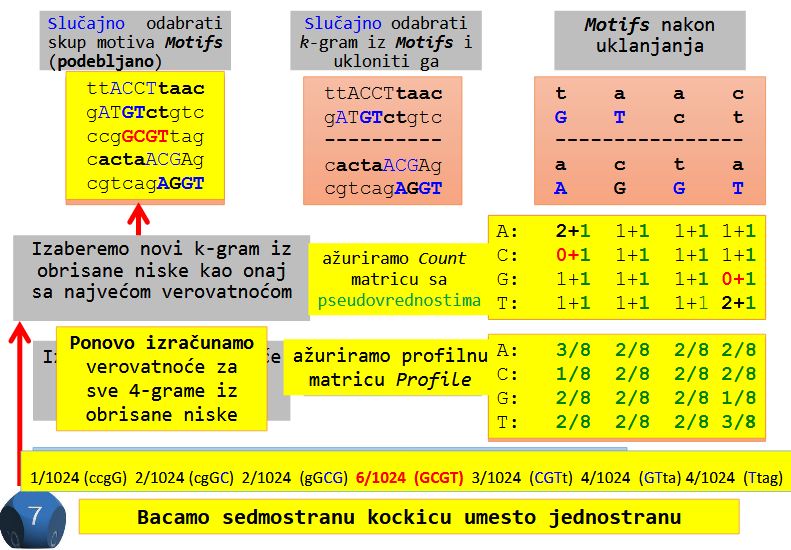
\includegraphics[width=0.7\textwidth]{poglavlja/2/slike/84.PNG}
\caption{Primer rada Gibsovog sempliranja sa primenom Laplasovog pravila}
\label{slika: gibs i laplas}
\end{figure}

\subsection{Koji princip odabrati?}
Odgovor na ovo pitanje je - nema pravila. Nekada će se bolje pokazati jedan, a nekada drugi. Najbolje je da isprobamo više algoritama i vidimo koji se najbolje ponaša u našem slučaju. Možemo koristiti već zapažene prednosti i mane u izboru, kao na primer biranje \textit{Median string} algoritma pri malim vrednostima $k$, ali isprobavanje je ipak najpouzdaniji pristup.


\chapter{Kako složiti genomsku slagalicu od milion delova?}
\setbookcodestyle

U ovom poglavlju predstavi\'cemo dati problem i prikazati kako mo\v zemo primeniti grafovske algoritme nad problemom slaganja genomske slagalice. Poglavlje \'cemo zapo\v ceti pri\v com o sekvenciranju genoma. Do sada smo videli \v sta za nas zna\v ci pojam DNK -- da se podsetimo, to je niska karaktera nad azbukom $\Sigma = \{A, C, G, T\}$. Biolo\v ski posmatrano, DNK je molekul koji se nalazi u svakoj \'celiji svakog organizma i da je u njemu zapisan na\v cin pravilnog razvoja i funkcionisanja svakog organizma. 

\section{Šta je sekvenciranje genoma?}

Sa biološke strane, genom jednog organizma predstavlja njegov genetski materijal. Pod genetskim materijalom podrazumevamo delove genoma koji se nasle\dj uju koji se nasle\dj uje i koji svi predstavnici jedne vrste dele u velikoj meri. Kod većine organizama, genetski materijal je sadržan u DNK, odnosno, genom je ekvivalentan sa DNK molekulima. Kod nekih drugih organizama koji su u manjini, kao \v sto su, na primer, virusi, va\v zi da oni ne sadr\v ze DNK i njihov genetski materijal se nalazi u ribonukleinskoj kiselini -- RNK -- o kojoj \'ce biti re\v ci u nastavku. 

Kod čoveka, genom sadrži oko tri milijarde nukleotida. Dakle, sa računarske strane posmatrano genom je niska karaktera nad azbukom $\Sigma = \{A, C, G, T\}$. Kompleksnost organizma nije u relaciji sa veli\v cinom genoma. Genomi nekih organizama su i stotinu puta veći od humanog genoma. Na primer, jedna vrsta amebe ima 670 milijardi nukleotida ili jedna vrsta kaktusa koja raste u Japanu ima 150 milijardi nukleotida.

Sekvenciranje genoma podrazumeva otkrivanje sastava genoma. U pitanju je eksperimentalan proces -- da bismo saznali \v sta se nalazi u sastavu jednog genoma, potreban nam je uzorak tkiva odgovaraju\'ce vrste. U nastavku dajemo kratak pregled razvoja sekvenciranja genoma.

\subsection{Kratka istorija sekvenciranja genoma}

Kao \v sto smo videli, sekvenciranje genoma je eksperimentalan proces, za koji je neophodna veoma sofisticirana tehnologija. Pre svega mo\v zemo govoriti o razvoju fizi\v cko-hemijskih tehnika koje bi dovele do mogu\'cnosti saznavanja sastava genoma. Walter Gilbert i Frederick Sanger su 1977. godine razvili nezavisne metode sa sekvenciranje genoma, za koje su, 1980. godine, podelili Nobelovu nagradu. Me\dj utim, iako su njihovi metodi bili pionirski u ovoj oblasti, njihove metode za sekvenciranje su bile veoma skupe -- za sekvenciranje humanog genoma je bilo potrebno 3 milijarde dolara.

Krajem 2000-ih Sanger metodom je sekvencioniran veliki broj genoma. Visoka cena je bila ograničavajući faktor i za dalji napredak je bila neophodna nova tehnologija sekvencioniranja. \emph{NGS} (skr. \emph{Next Generation Sequencing}) predstavlja metode nove generacije sekvencioniranja, odnosno, novu generaciju ma\v sina sekvencera koji vr\v se sekvencioniranje. \emph{Illumina}, jedan od proizvo\dj a\v ca sekvencera, smanjuje trošak sekvencioniranja humanog genoma sa 3 milijarde na 10 hiljada dolara. Kompanija \emph{Complete Genomics} otvara genomsku fabriku u Silikonskoj dolini koja sekvencionira stotine genoma mesečno. Pekinški genomski institut (\emph{Beijing Genome Institute}, skr. \emph{BGI}) preuzima Complete Genomics 2013. godine i postaje najveći svetski centar za sekvenciranje genoma. Na slici \ref{slika:cena} prikazano je kako se cena sekvencioniranja menjala godinama.

\iffalse
\begin{figure}[h]
	\centering
	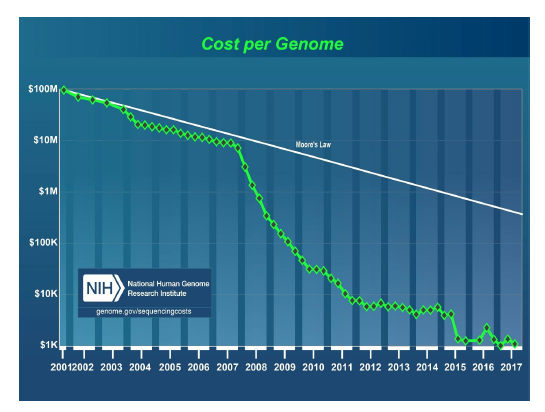
\includegraphics[width=0.95\textwidth]{poglavlja/3/slike/cena_sekvencioniranja.png}
	\caption{Cena sekvencioniranja kroz istoriju.}
	\label{slika:cena}
\end{figure} 
\fi 

\subsection{Sekvenciranje ličnih genoma}

Prirodno je zapitati se o značaju poznavanja sastava genoma. \v Sto je ti\v ce biljaka, neke od primena sekvenciranja su: razvoj novih biljnih vrsta u poljoprivredi, odre\dj ivanje pogodnog podneblja za neku biljnu vrstu, u farmaciji, i dr. Me\dj utim, najzna\v cajnija primena je u sekvenciranju li\v cnih genoma.

Genomi se kod različitih ljudi razlikuju na malom broju pozicija (u proseku sadrže jednu mutaciju na hiljadu nukleotida). Ova razlika je odgovorna za, na primer, različite visine kod ljudi, da li će imati sklonost ka visokom holesterolu ili ne, za veliki broj genetskih bolesti, itd.

Godine 2010. Nicholas Volker je postao prvo ljudsko biće čiji je život spašen zahvaljujući genomskom sekvencioniranju. Lekari nisu mogli da postave tačnu dijagnozu i morali su da ga podvrgnu velikom broju operacija pokušavajući da je utvrde. Sekvenciranje je otkrilo retku mutaciju na jednom genu (XIAP) koja je bila povezana sa oštećenjem njegovog imunog sistema. Ovo otkriće je navelo lekare na adekvatnu terapiju koja je rešila problem.

\section{Eksplozija u štampariji}

Razmotrimo slede\'ci primer. Neka imamo hiljadu kopija istog izdanja novina na jednoj gomili, a ispod njih postavljen je dinamit. Upalimo fitilj i zamislimo da nije sve samo izgorelo već da se raspršilo u milione delića papira. Kako možemo da iskoristimo te deliće da bismo saznali koje su bile vesti iz tog izdanja? Ovaj problem nazvaćemo \emph{Problem novina} (videti sliku \ref{slika:eksplozija}). 

\iffalse 
\begin{figure}[h]
	\centering
	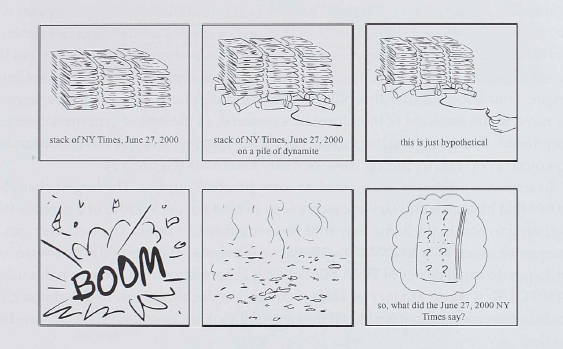
\includegraphics[width=1\textwidth]{poglavlja/3/slike/eksplozija.png}
	\caption{Problem novina poslužiće nam u razumevanju problema slaganja genoma.}
	\label{slika:eksplozija}
\end{figure} 

\fi 

Problem novina je mnogo teži nego što izgleda. Kako smo imali više kopija istog izdanja, i kako smo izgubili neki deo informacija prilikom eksplozije, ne možemo samo da prilepimo deliće novina kao da su slagalica. Umesto toga, potrebno je da preklopimo delove različitih novina kako bismo rekonstruisali jedan primerak.

\iffalse 
\begin{figure}[h]
	\centering
	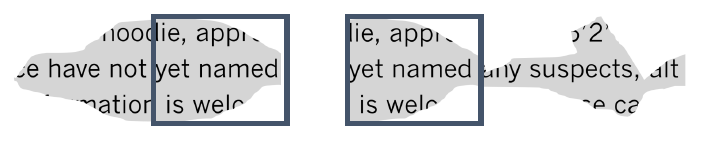
\includegraphics[width=1\textwidth]{poglavlja/3/slike/delici.png}
	\caption{Spajanje delova različitih novina koji se jednim delom preklapaju.}
	\label{slika:delici}
\end{figure} 
\fi 

Određivanje redosleda nukleotida u genomu, odnosno sekvenciranje genoma, predstavlja bitan problem u bioinformatici. Ve\'c smo pomenuli da dužine genoma variraju -- humani genom je dugačak oko 3 milijarde nukleotida, dok je genom jednoćelijskog organizma \emph{Amoeba dubia} čak 200 puta duži. 

Razmotrimo sada povezanost problema novina i sekvenciranja genoma. Kopije izdanja u problemu novina odgovaraju ono predstavlja ulaz u sekvencerima -- uzorak tkiva. Moderne mašine za sekvenciranje ne mogu da pročitaju ceo genom nukleotid po nukleotid od početka do kraja (kao što bismo pročitali knjigu). Mogu samo da iseckaju genom i generišu njegova kratka \emph{očitavanja} (engl. \emph{reads}). Kako to zapravo funkcioniše? 

Na slici \ref{slika:sekvenciranje} ilustrovan je proces sekvenciranja. Sekvencer dobija milione kopija istog genoma. Zatim vrši očitavanja čime dobijamo deliće odnosno kratke podniske. Neki delovi odnosno očitavanja biće izgubljena (kao delići novina u eksploziji, dakle gubimo deo informacija). Očitavanja su izmešana i ono što nam sekvencer daje je zapravo kolekcija podniski koje treba spojiti u jednu. Sastavljanje genoma nije isto kao i slaganje slagalice -- moramo da koristimo preklapajuća očitavanja da bismo rekonstruisali genom.

\iffalse
\begin{figure}[h]
	\centering
	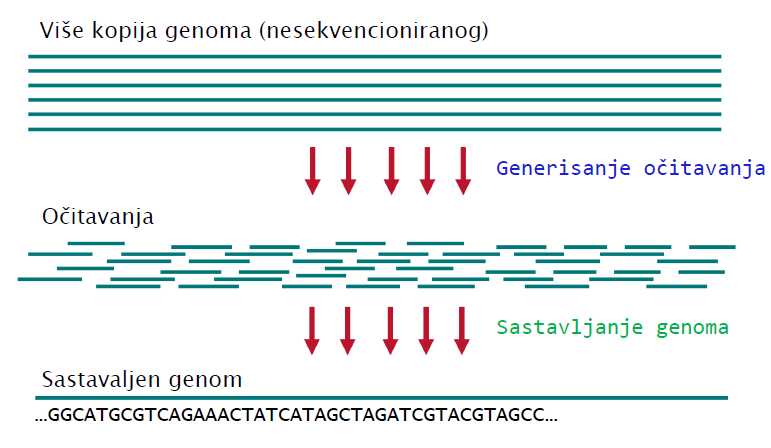
\includegraphics[width=1\textwidth]{poglavlja/3/slike/sekvencioniranje.png}
	\caption{Ilustracija problema.}
	\label{slika:sekvenciranje}
\end{figure} 
\fi 

\section{Problem sekvenciranja genoma}

Do sada smo videli \v sta predstavlja sekvenciranje genoma, koja je njegova biolo\v ska podloga i kako se on defini\v se kao biolo\v ski problem. Pre\dj imo sada na formulisanje ra\v cunarskog problema sekvenciranja genoma kao problem rekonstrukcije niske.

\begin{tcolorbox}
	\textbf{Problem sekvencioniranja genoma:} Rekonstruisati genom na osnovu očitavanja. \\
	\textit{Ulaz:} Kolekcija niski \emph{Reads}.\\
	\textit{Izlaz:} Niska \emph{Genome} rekonstruisana na osnovu \emph{Reads}.
\end{tcolorbox}

Ovo nije dobro definisan problem. Potrebno je uvesti dodatne pojmove kako bismo uspeli da problem sekvencioniranja genoma predstavimo kao problem rekonstrukcije niske.

Defini\v semo pojam \emph{$k$-gramski sastav niske} na slede\'ci na\v cin. $k$-gramski sastav niske $Text$, u oznaci $Composition_k(Text)$, predstavlja kolekciju podniski dužine $k$ niske $Text$, pri \v cemu su u kolekciju uključeni duplikati. Na primer, neka je $Text=TAATGCCATGGGATGTT$. Njen $3$-gramski sastav niske $Text$ izgleda:

\begin{lstlisting}
Composition_3(TAATGCCATGGGATGTT) =
              TAA 
               AAT 
                ATG
                 TGC
                  GCC
                   CCA
                    CAT
                     ATG
                      TGG
                       GGG
                        GGA
                         GAT
                          ATG
                           TGT
                            GTT
\end{lstlisting}

\noindent odnosno, ako kolekciju uredimo po leksikografskom pore\dj enju:

\begin{lstlisting}
Composition_3(TAATGCCATGGGATGTT) =
AAT ATG ATG ATG CAT CCA GAT GCC GGA GGG GTT TAA TGC TGG TGT
\end{lstlisting}

\noindent Sada možemo malo bolje da definišemo problem.

\begin{tcolorbox}
	\textbf{Problem rekonstrukcije niske:} Rekonstruisati nisku na osnovu njenog $k$-gramskog sastava. \\
	\textit{Ulaz:} Kolekcija $k$-grama.\\
	\textit{Izlaz:} Niska \emph{Genome} takva da je $Composition_k(Genome)$ ekvivalentno kolekciji $k$-grama.
\end{tcolorbox}
~

Zapo\v cnimo prvo sa naivnim pristupom re\v savanju ovog problema. Odaberimo jedan $k$-gram za početni. Zatim nižemo ostale tako da se sufiks poslednjeg odabranog poklopi sa prefiksom nekog od preostalih $k$-grama. Pri tome, ako ima više takvih $k$-grama, biramo proizvoljan jedan. Na ovaj način možemo doći do rešenja, ali je veoma skupo. Pri tome, velika je šansa da ćemo se negde zaglaviti (tj. nijedan od preostalih $k$-grama neće biti kandidat za nadovezivanje na tekuću nisku) ili zbog izbora početnog $k$-grama ili zbog izbora nekog od preostalih $k$-grama kada je postojalo više odgovarajućih. Sledeći primer ilustruje ovaj problem.

Neka nam je dat sledeći 3-gramski sastav: \texttt{AAT ATG ATG ATG CAT CCA GAT GCC GGA GGG GTT TAA TGC TGG TGT}. Treba rekonstruisati nisku koja ima takav sastav. Biramo početni 3-gram, neka to bude na primer \texttt{TAA}. Zatim na njega treba nadovezati 3-gram koji počinje njegovim sufiksom dužine 2, odnosno onaj 3-gram koji ima prefiks \texttt{AA}. U našem slučaju, postoji jedan takav 3-gram i njega nadovezujemo na tekuću nisku, tako da sada imamo \texttt{TAAT}. Zatim biramo 3-gram čiji je prefiks \texttt{AT}. Ovog puta imamo 3 kandidata, ali, na našu sreću, sva tri su isti 3-grami, \texttt{ATG}. U takvom slučaju nije bitno koji smo odabrali, jer su svi jednaki. Nadovezujemo ga na tekuću nisku i dobijamo \texttt{TAATG}. Tražimo 3-grame sa prefiksom \texttt{TG}, koji do sad nisu upotrebljeni. Ponovo pronalazimo 3 kandidata. Međutim, u ovom slučaju, svi kandidati predstavljaju različite 3-grame, a to su \texttt{TGC}, \texttt{TGG} i \texttt{TGT}. Naivni pristup kaže da biramo jedan od njih, i recimo da smo odabrali \texttt{TGT} i dobili nisku \texttt{TAATGT}. Sada nam je potreban 3-gram sa prefiksom \texttt{GT} i tu dolazi do zaglavljivanja. Imamo još 3-grama koji nisu iskorišćeni za rekonstrukciju niske, ali nijedan ne možemo da iskoristimo u ovom trenutku. U takvim situacijama treba se vratiti u nazad do koraka u kom je bilo više kandidata.

\section{Rekonstrukcija niske kao problem Hamiltonove putanje}

Videli smo da nam naivni pristup ne odgovara i moramo smisliti bolje rešenje. Mogli bismo da iskoristimo znanja iz teorije grafova za rešavanje ovakvog problema. U tom slučaju, prvi zadatak je da našu nisku predstavimo u vidu grafa.

\subsection{Genom kao putanja}

Vratimo se na prethodni primer. Dat nam je naredni 3-gramski sastav:
\begin{lstlisting}
Composition_3(TAATGCCATGGGATGTT) =
              TAA 
               AAT 
                ATG
                 TGC
                  GCC
                   CCA
                    CAT
                     ATG
                      TGG
                       GGG
                        GGA
                         GAT
                          ATG
                           TGT
                            GTT
\end{lstlisting}

Ovakav 3-gramski sastav mo\v zemo predstaviti kao graf na slede\'ci na\v cin. Svakom \v cvoru u grafu odgovara jedan od $k$-grama. Zatim, potrebne su nam grane koje će povezati te čvorove. Dva čvora su povezana usmerenom granom ako izlazni čvor ima sufiks koji je jednak prefiksu ulaznog čvora te grane, kao što je prikazano na slici \ref{slika:hamilton}.

\begin{figure}[H]
	\centering
	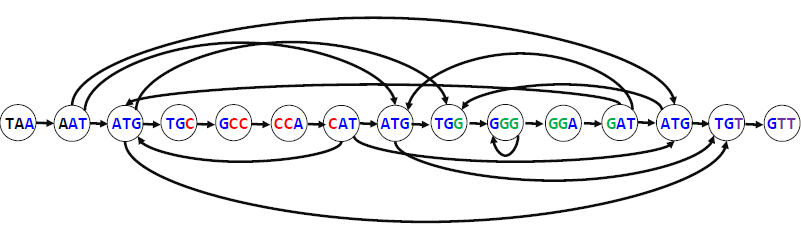
\includegraphics[width=1\textwidth]{poglavlja/3/slike/hamilton.png}
	\caption{Graf koji odgovara 3-gramskom sastavu niske $TAATGCCATGGGATGTT$.}
	\label{slika:hamilton}
\end{figure} 

Jasno je da postoji više puteva u ovom grafu. Postavlja se pitanje -- da li možemo da pronađemo genomsku putanju u ovom grafu, od svih koje postoje?

Podsetimo se šta je Hamiltonova putanja. Hamiltonova putanja je putanja koja posećuje svaki čvor u grafu tačno jednom. To je upravo ono što nam je potrebno za rešavanje problema. Svaki čvor predstavlja jedan $k$-gram i potrebno nam je da svi $k$-grami budu uključeni u rekonstruisanu nisku tačno jednom.
~ \\
\begin{tcolorbox}
	\textbf{Problem Hamiltonove putanje:} Naći Hamiltonovu putanju u grafu. \\
	\textit{Ulaz:} Graf.\\
	\textit{Izlaz:} Putanja koja posećuje svaki čvor u grafu tačno jednom.
\end{tcolorbox}

~\\

Iako deluje kao da smo rešili sve probleme, zapravo smo naišli na još jednu veliku prepreku. Naime, pronalaženje Hamiltonovog puta u grafu je NP-kompletan problem, što znači da ne postoji algoritam koji ga rešava u polinomijalnom vremenu. U tom slučaju, moramo da se vratimo na početak, a to je predstavljanje $k$-gramskog sastava grafom.

\section{Rekonstrukcija niske kao Ojlerove putanje}

U prethodnoj sekciji, $k$-grame smo predstavili čvorovima u grafu i u njemu tražili Hamiltonov put, odnosno, put koji obilazi svaki čvor tačno jednom. Videli smo da za taj problem još uvek nije poznat efikasan algoritam pa se sada pitamo kako možemo izmeniti graf tako da ne zahteva traženje Hamiltonove putanje.

Ono što se javlja kao ideja jeste obeležavanje grana umesto čvorova. Dakle, svaka grana biće obeležena jednim $k$-gramom. Izlazni čvor biće obeležen prefiksom $k$-grama te grane, dok će ulazni čvor biti obeležen sufiksom istog tog $k$-grama. Slika \ref{slika:ojler} ilustruje ovaj postupak za nisku $TAATGCCATGGGATGTT$.

\begin{figure}[h]
	\centering
	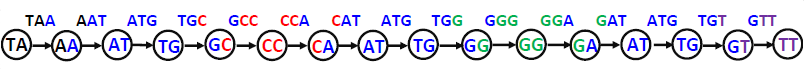
\includegraphics[width=1\textwidth]{poglavlja/3/slike/ojler.png}
	\caption{Graf koji odgovara 3-gramskom sastavu niske $TAATGCCATGGGATGTT$. Grane su obeležene 3-gramima, a čvorovi 2-gramima koji predstavljaju prefikse i sufikse.}
	\label{slika:ojler}
\end{figure} 

Primećujemo da su neki čvorovi obleženi identično (na primer, imamo tri čvora sa oznakom $AT$). Sve čvorove koji imaju istu oznaku treba spojiti u jedan, pri čemu zadržavamo sve grane koje su ulazile u taj čvor ili su izlazile iz njega. Ponavljamo postupak dokle god imamo čvorove koji imaju istu oznaku i na kraju dobijamo graf koji nazivamo \emph{De Brojnov graf}. Slika \ref{slika:debrojnov} ilustruje De Brojnov graf dobijen ovom procedurom od polaznog grafa sa slike \ref{slika:ojler}. 

\begin{figure}[h]
	\centering
	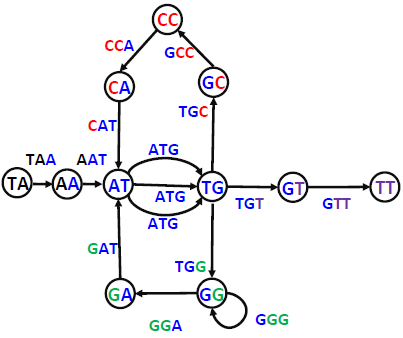
\includegraphics[width=0.55\textwidth]{poglavlja/3/slike/debrojnov.png}
	\caption{De Brojnov graf koji odgovara niski $TAATGCCATGGGATGTT$.}
	\label{slika:debrojnov}
\end{figure} 

Ovime smo dobili novu reprezentaciju niske pomoću grafa. Prirodno se postavlja naredno pitanje -- gde se nalazi niska \textit{Genome} u ovoj reprezentaciji grafa? Kako nam se 3-grami sada nalaze na granama, a ne u čvorovima, potrebno je da pronađemo putanju u grafu koja prolazi sve grane tačno jednom. Takav put nazivamo \emph{Ojlerova putanja}. Srećom, algoritam za pronalaženje Ojlerove putanje u grafu nije NP-kompletan i možemo efikasno da je pronađemo.
~ \\
\begin{tcolorbox}
	\textbf{Problem Ojlerove putanje:} Pronaći Ojlerovu putanju u grafu. \\
	\textit{Ulaz:} Graf.\\
	\textit{Izlaz:} Putanja koja posećuje svaku granu u grafu tačno jednom.
\end{tcolorbox}

~\\

Sada znamo kako možemo da dobijemo nisku kada znamo De Brojnov graf koji odgovara njenom $k$-gramskom sastavu. Međutim, konstruisali smo De Brojnov graf na osnovu genoma, ali u realnim primenama, genom je nepoznat.

\section{De Brojnovi grafovi na osnovu kolekcije $k$-grama}

Videli smo kako mo\v zemo od zadate niske prona\'ci De Brojnov graf. Na\v zalost, u primenama nije nam poznata niska, ali znamo njen $k$-gramski sastav. Postavlja se pitanje kako mo\v zemo konstruisati De Brojnov graf od $k$-gramskog sastava niske. 

Za svaki $k$-gram pravimo dva čvora i jednu granu -- oznaka grane je upravo taj $k$-gram, oznaka izlaznog \v cvora je prefiks, a ulaznog \v cvora je sufiks datog $k$-grama. Time dobijamo nepovezani graf kao na slici \ref{slika:kgrami}. Zatim lepimo identične čvorove sve dok ne dobijemo graf čiji svi čvorovi imaju različite oznake. Na slici \ref{slika:lepljenje} dat je jedan korak ovog postupka, međutim, tu nije kraj jer i dalje postoje čvorovi sa istim oznakama.

\begin{figure}[h]
	\centering
	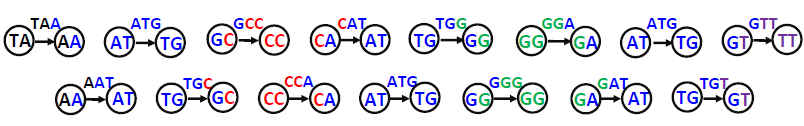
\includegraphics[width=1\textwidth]{poglavlja/3/slike/debrojnov1.png}
	\caption{Svaki k-gram prestavljen je pomoću dva čvora i jedne grane.}
	\label{slika:kgrami}
\end{figure} 

\begin{figure}[h]
	\centering
	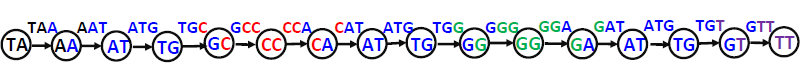
\includegraphics[width=1\textwidth]{poglavlja/3/slike/lepljenje.png}
	\caption{Prvi korak u postupku lepljenja čvorova. Napomenimo da postupak nije završen jer treba zalepiti čvorove sa identičnim oznakama (na primer, AT).}
	\label{slika:lepljenje}
\end{figure} 

Po završetku postupka dobijamo de Brojnov graf koji je isti kao onaj koji smo dobili kada smo znali nisku, odnosno, graf na slici \ref{slika:debrojnov}. Svaka grana je označena jednim $k$-gramom, a svaki čvor je označen prefiksom, odnosno, sufiksom odgovaraju\'ce izlazne, odnosno, ulazne grane, redom. Naravno, \v cvovori koji imaju identi\v cne oznake su zalepljeni.

\section{Ojlerova teorema}

Za re\v savanje problema Ojlerove putanje koji smo predstavili u prethodnoj sekciji mo\v zemo iskoristiti re\v senje narednog problema. Ovaj problem je zna\v cajan jer postoji teorema koja ga prati, a koja odre\dj uje uslove za njegovo re\v savanje.

\begin{tcolorbox}
	\textbf{Problem Ojlerovog ciklusa:} Pronaći Ojlerov ciklus u grafu. \\
	\textit{Ulaz:} Graf.\\
	\textit{Izlaz:} Ciklus koji posećuje svaku granu u grafu tačno jednom.
\end{tcolorbox}



Ka\v zemo da je graf Ojlerov ako sadr\v zi Ojlerov ciklus. Ispostavlja se da postoje odre\dj ene karakteristike koje odre\dj uju da li je graf Ojlerov. Uvedimo pojmove povezan graf i balansiran graf. Kažemo da je graf \emph{povezan} ako za ma koja dva čvora postoji putanja koja ih povezuje. Graf je \emph{balansiran} ako za svaki čvor važi da mu je izlazni stepen jednak ulaznom. Naredna teorema govori o potrebnim i dovoljnim uslovima da graf bude Ojlerov.

\begin{teorema}[Ojlerova teorema]
	Svaki Ojlerov graf je balansiran. Svaki povezan graf i balansiran graf je Ojlerov.
\end{teorema}

\subsection{Dokaz Ojlerove teoreme}

Neka nam je dat povezan balansiran graf. Da bismo pokazali da graf sadrži Ojlerov ciklus, postavićemo mrava na bilo koji od čvorova tog grafa, kao na slici \ref{slika:mrav1}. Zašto baš mrav? Poznato je da mravi nikada ne idu istim putem dva puta pa smo sigurni da će naš mrav proći svaku granu tačno jednom.

Puštamo mrava da slučajno odabira grane kojima će se kretati. Ako je veoma pametan, obići će svaku granu jednom i vratiće se u početni čvor. Međutim, velike su šanse da nije veoma pametan i da će se u nekom čvoru zaglaviti, odnosno, neće imati granu koju već nije obišao.

Da li mrav može da se zaglavi u bilo kom čvoru? Ispostavlja se da može da se zaglavi samo u početnom čvoru (jer je graf balansiran). U trenutku kada se zaglavio on je napravio ciklus. Samo, taj ciklus nije Ojlerov jer još uvek nije obišao sve grane. Ideja je da odabere drugačiji početni čvor iz kog će krenuti obilazak. Koji čvor će izabrati? Treba da izabere čvor iz ciklusa koji ima izlaznih grana koje još uvek nije obišao (slika \ref{slika:mrav2}). 

\noindent
\begin{minipage}{\textwidth}
	\centering
	\begin{minipage}{0.45\textwidth}
		\begin{figure}[H]
			\centering
			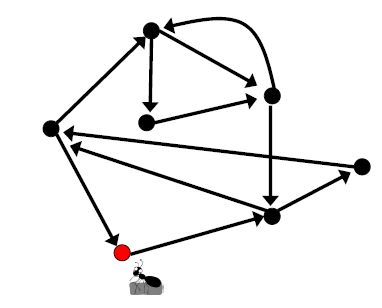
\includegraphics[width=\textwidth]{poglavlja/3/slike/mrav1.png}
			\caption{Mrav je postavljen u crveni čvor i odatle kreće obilazak povezanog balansiranog grafa.}
			\label{slika:mrav1}
		\end{figure} 
	\end{minipage}
	\hfill 
	\begin{minipage}{0.45\textwidth}
		\begin{figure}[H]
			\centering
			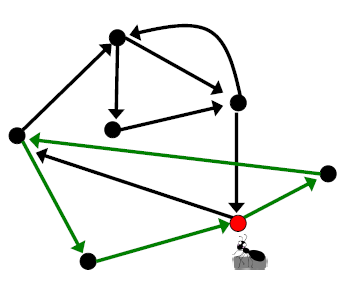
\includegraphics[width=\textwidth]{poglavlja/3/slike/mrav2.png}
			\caption{Mrav se zaglavio i pokušava ponovo iz drugog čvora koji pripada ciklusu i ima izlazne grane koje nisu posećene.}
			\label{slika:mrav2}
		\end{figure} 
	\end{minipage}
	\vspace*{1em}
\end{minipage}

Sada, mrav pokušava ispočetka iz novog čvora. Prvo obilazi ciklus koji je već pronašao u prethodnom pokušaju, a zatim nastavlja obilazak preko neposećenih grana. Na taj način, ciklus se uvećava dok se ne dođe do Ojlerovog. Ukoliko se ponovo zaglavi (slika \ref{slika:mrav3}) ponovo bira novi početni čvor, obilazi pronađeni ciklus (koji i dalje nije Ojlerov) i tako sve dok ne uspe da obiđe sve grane (slika \ref{slika:mrav4}).

Dokaz Ojlerove teoreme daje primer konstruktivnog dokaza, koji ne dokazuje samo željeni rezultat, već pruža metod za konstrukciju onoga što nam je potrebno. Ukratko, pratili smo kretanje mrava dok nije pronašao Ojlerov ciklus u povezanom balansiranom grafu, što je sumirano u algoritmu \texttt{EulerianCycle}.

\noindent
\begin{minipage}{\textwidth}
	\centering
	\begin{minipage}{0.45\textwidth}
		\begin{figure}[H]
			\centering
			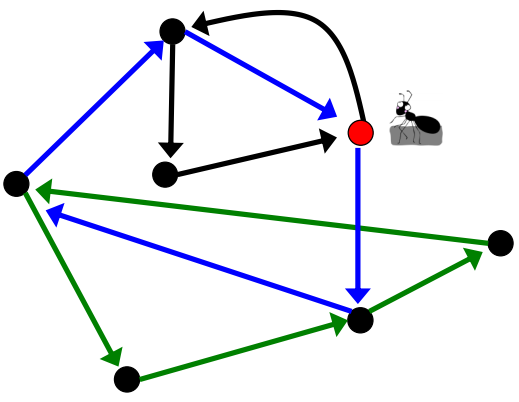
\includegraphics[width=\textwidth]{poglavlja/3/slike/mrav3.png}
			\caption{Mrav se ponovo zaglavio i pokušava od novog čvora.}
			\label{slika:mrav3}
		\end{figure} 
	\end{minipage}
	\hfill 
	\begin{minipage}{0.45\textwidth}
		\begin{figure}[H]
			\centering
			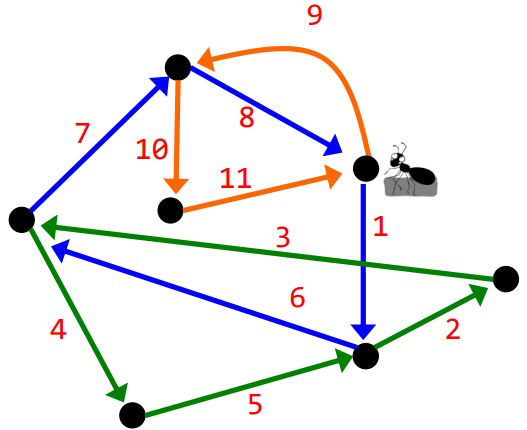
\includegraphics[width=\textwidth]{poglavlja/3/slike/mrav4.png}
			\caption{Mrav je konačno uspeo da pronađe dobar početni čvor i Ojlerov ciklus. Grane su obeležene redosledom kojim su posećene.}
			\label{slika:mrav4}
		\end{figure} 
	\end{minipage}
	\vspace*{1em}
\end{minipage}

\begin{lstlisting}
EulerianCycle(BalancedGraph)
begin
	form a Cycle by randomly walking in BalancedGraph (avoiding already visited edges)
	while Cycle is not Eulerian
		select a node newStart in Cycle with still unexplored outgoing edges
		form a Cycle' by traversing Cycle from newStart and randomly walking afterwards
		Cycle %$\leftarrow$% Cycle'
	return Cycle
end
\end{lstlisting}

Ovaj algoritam radi u linearnom vremenu. Da bi se zaista postigla ta efikasnost, potrebne su efikasne struktutre podataka za održavanje ciklusa koje mrav pronalazi kao i za liste neiskorišćenih grana za svaki čvor i lista čvorova u trenutnom ciklusu koji imaju neiskorišćene grane.

\section{Sastavljanje parova očitavanja}

Predstavimo kao da su svi naši problemi rešeni. Međutim, može se javiti više Ojlerovih putanja u grafu. Srećom, i za ovo imamo jednostavno rešenje.

\subsection{DNK sekvenciranje sa parovima očitavanja} 

Imamo više identičnih kopija genoma i na slučajnim pozicijama sečemo genom na fragmente iste dužine \textit{InsertLength}. Zatim generišemo \emph{parove očitavanja} -- dva očitavanja sa krajeva svakog fragmenta na jednakoj, fiksiranoj udaljenosti. Pod \emph{uparenim $k$-gramom} podrazumevamo par $k$-grama na fiksiranom rastojanju $d$ u genomu. \emph{Upareni $k$-gramski sastav}, u oznaci $PairedComposition_k(Text)$, sastoji se od svih $k$-grama niske $Text$ i njihovih parova.

\begin{figure}[h]
	\centering
	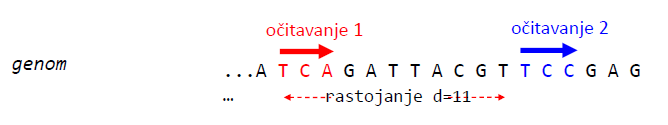
\includegraphics[width=1\textwidth]{poglavlja/3/slike/upareni_kgram.png}
	\caption{\texttt{TCA} i \texttt{TCC} na rastojanju $d=11$ čine jedan upareni 3-gram.}
	\label{slika:upareni}
\end{figure} 

Dajmo jedan primer. Neka imamo nisku \texttt{TAATGCCATGGGATGTT}, i upareni 3-gram \texttt{TAA} i \texttt{GCC}. Upareni $k$-gramski sastav date niske prikazan je na slici \ref{slika:upareni3}.

\begin{figure}[h]
	\centering
	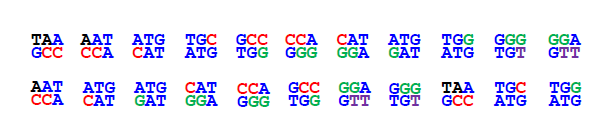
\includegraphics[width=1\textwidth]{poglavlja/3/slike/upareni_3gram.png}
	\caption{\emph{PairedComposition} niske \texttt{TAATGCCATGGGATGTT} i njegov leksikografski poredak.}
	\label{slika:upareni3}
\end{figure} 

Sada mo\v zemo formulisati naredni problem.

~ \\
\begin{tcolorbox}
	\textbf{Problem rekonstrukcije niske na osnovu parova očitavanja:}	Rekonstruisati nisku na osnovu njenih uparenih $k$-grama. \\
	\textit{Ulaz:} Kolekcija uparenih $k$-grama.\\
	\textit{Izlaz:} Niska $Text$ takva da je $PairedComposition_k(Text)$ jednak kolekciji uparenih $k$-grama. 
\end{tcolorbox}
~\\

Kako konstruisati upareni De Brojnov graf na osnovu uparenog $k$-gramskog sastava? Postupak je sličan prethodnom slučaju, kada nismo imali parove. Pretpostavimo da je dat genom (niska $Genome$). Posmatrajmo genom kao putanju u grafu obeleženom na osnovu njegovog uparenog $k$-gramskog sastava (videti sliku \ref{slika:upareniDeBrojnov}). Svaka grana obeležena je uparenim $k$-gramom, a svaki čvor uparenim prefiksom, odnosno, sufiksom $k$-grama.

\begin{figure}[h]
	\centering
	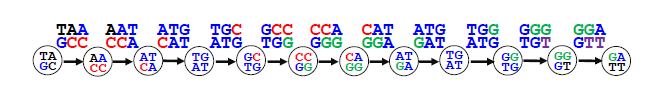
\includegraphics[width=1\textwidth]{poglavlja/3/slike/upareni_debrojnov.png}
	\caption{Graf koji odgovara uparenom 3-gramskom sastavu niske \texttt{TAATGCCATGGGATGTT}.}
	\label{slika:upareniDeBrojnov}
\end{figure} 

Potrebno je zalepiti čvorove sa istom oznakom, tako da svi čvorovi budu jedinstveno obeleženi. Postupak je identičan prethodnom slučaju, odnosno, kada nismo imali parove. Primetimo da sada imamo mnogo manje lepljenja jer imamo samo dva čvora sa istom oznakom (\texttt{TG} \texttt{AT}), (videti sliku \ref{slika:uparenoLepljenje}).

\begin{figure}[h]
	\centering
	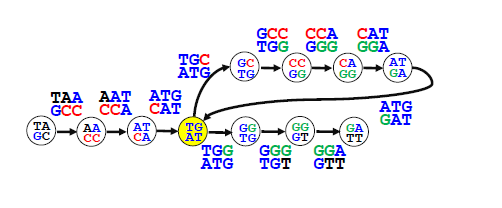
\includegraphics[width=1\textwidth]{poglavlja/3/slike/upareno_lepljenje.png}
	\caption{Dva čvora sa oznakom (\texttt{TG AT}) spajaju se u jedan pri čemu su sve grane, incidentne sa tim čvorovima, očuvane.}
	\label{slika:uparenoLepljenje}
\end{figure} 

Kao i u prethodnom slučaju, pretpostavili smo da je dat genom (niska $Genome$), što često nije slučaj. Posmatrali smo genom kao putanju u grafu obeleženom na osnovu njegovog uparenog $k$-gramskog sastava. Sada pretpostavimo da nije dat genom već samo upareni $k$-gramski sastav. Za svaki upareni $k$-gram pravimo dva čvora i jednu granu, zatim lepimo identične čvorove (videti \ref{slika:uparenoLepljenje2}), i na kraju dobijamo upareni De Brojnov graf, kao onaj na slici \ref{slika:uparenoLepljenje}.

\begin{figure}[H]
	\centering
	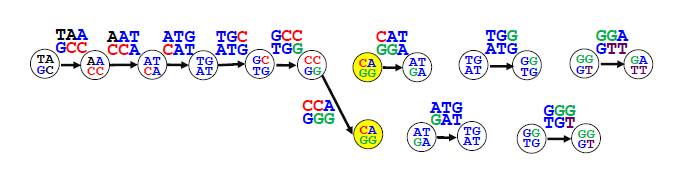
\includegraphics[width=1\textwidth]{poglavlja/3/slike/upareno_lepljenje2.png}
	\caption{Konstrukcija uparenog De Brojnovog grafa na osnovu uparenih $k$-grama.}
	\label{slika:uparenoLepljenje2}
\end{figure} 

Dakle, upareni De Brojnov graf, na osnovu kolekcije uparenih $k$-grama, dobijamo tako što svaku granu označavamo jednim uparenim $k$-gramom. Zatim, svaki čvor označavamo prefiksima, odnosno, sufiksima odgovaraju\'ce izlazne, odnosno, ulazne grane, redom. Na kraju, lepimo čvorove sa identičnim oznakama.

\section{U realnosti}
Ovde smo imali neke nerealne pretpostavke:
\begin{itemize}
	\item Savršena pokrivenost genoma očitavanjima (svaki $k$-gram iz genoma je očitan). Očitavanja dužine 250 nukleotida dobijena \emph{Illumina} tehnologijom predstavljaju samo mali deo 250-grama unutar genoma. Rešenje je u razbijanju dobijenih očitavanja na kraće $k$-grame (kao na slici \ref{slika:manji kgrami}).
	\item Očitavanja ne sadrže greške. U ovom slu\v caju, ako bismo razbili na manje $k$-grame, onda bismo dobili vi\v se niski koje imaju pogre\v sno o\v citavanje. Postavljamo pitanje kako se ovakvi slu\v cajevi manifestuju u konstrukciji DeBrojnovog grafa. Dolazi do stvaranja \emph{balon\v ci\'ca} (engl. \emph{bubble}) u grafu (videti sliku \ref{slika:baloncic}). Jednostavan je slu\v caj kada govorimo o gre\v sci na jednom o\v citavanju, me\dj utim, ukoliko postoji vi\v se gre\v saka, onda dolazi do \emph{eksplozije balon\v ci\'ca} (videti sliku \ref{slika:eksplozija baloncica}).
	\item Rastojanja između očitavanja u okviru parova očitavanja su egzaktna.
	\item itd.
\end{itemize}


\begin{figure}[h]
	\centering
	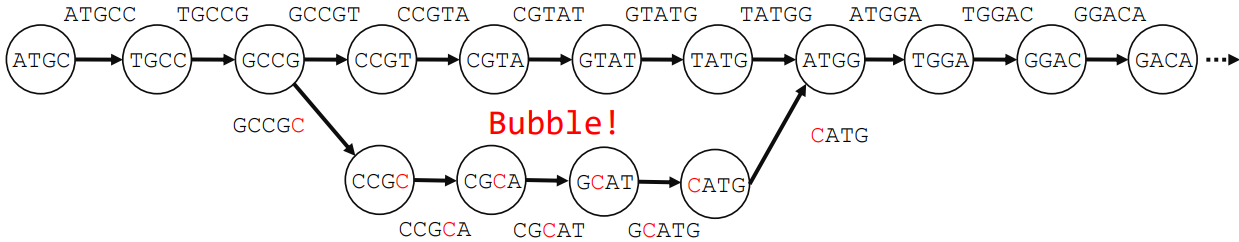
\includegraphics[width=\textwidth]{poglavlja/3/slike/baloncic.png}
	\caption{Primer pojave balon\v ci\'ca u De Brojnovom grafu usled pojave gre\v ske u o\v citavanju nukleotida \texttt{T} nukleotidom \texttt{C}.}
	\label{slika:baloncic}
\end{figure} 

\begin{figure}[h]
	\centering
	\includegraphics[width=\textwidth]{poglavlja/3/slike/razbijanje_na_manje_kgrame.png}
	\caption{Primer razbijanja dobijenih očitavanja na manje k-grame.}
	\label{slika:manji kgrami}
\end{figure}


\iffalse
\begin{figure}[H]
	\centering
	\includegraphics[width=0.5\textwidth]{poglavlja/3/slike/eksplozija-baloncica.png}
	\caption{Eksplozija balon\v ci\'ca.}
	\label{slika:eksplozija baloncica}
\end{figure}
\fi

\blankpage
\section{Maximal Non Branching Path}

Funkcija ima jedan parametar, \texttt{G} - de Bruijn graf. Funkcija vraća maksimalne nerazgranate putanje u grafu.

Putanja je inicijalno prazna lista, a dodatno održavamo mapu posećenih čvorova, koja je inicijalno prazna.

Za svaki čvor \texttt{v} u grafu \texttt{G} računamo ulazni i izlazni stepen (funkcijom \texttt{degree}). Ukoliko je jedan od ta dva različit od 1, obeležavamo da je čvor posećen. Dodatno, ukoliko je izlazni stepen veći od 0, želimo da obiđemo sve susede. Za svaki čvor \texttt{w} iz liste suseda čvora \texttt{v}, pravimo putanju koja na početku sadrži samo granu (v, w). Zatim, obeležimo da je čvor \texttt{w} posećen i računamo njegov ulazni izlazni stepen. 

Pošto nam je potreban nerazgranati put, pratimo čvorove koji imaju tačno jednu ulaznu i jednu izlaznu granu. Tako, dokle god su i ulazni i izlazni stepeni čvora \texttt{w} jednaki 1, određujemo čvor \texttt{u}, čvor koji se nalazi na drugom kraju izlazne grane iz čvora \texttt{w}. Tu granu treba dodati u trenutni put. Zatim, čvor \texttt{w} dobija vrednost čvora \texttt{u} i potrebno je ponovo označiti čvor \texttt{w} kao posećen i ažurirate stepene. Kada nema više čvorova koji ispunjavaju uslov, u listu putanja dodajemo trenutni put.

Još jednom prolazimo sve čvorove grafa \texttt{G}, i za svaki čvor \texttt{v} koji nije posećen, odredićemo izlovoani ciklus (funkcijom \texttt{isloated\_cycle}). Ukoliko takav ciklus postoji, dodajemo ga u listu putanja.



\lstinputlisting[language=Python, frame=single]{nedelje/4/kodovi/1.MaximalNonBranchingPath.py}


\subsection{Degree}
\label{degree}

Funkcija ima dva parametra, \texttt{G} - de Bruijn graf, i \texttt{v} - čvor čiji ulazni i izlazni stepen treba odrediti. Povratna vrednost je par ulazni i izlazni stepen čvora \texttt{v}.

Pošto je graf predstavljen kao mapa, koja preslikava čvorove u listu čvorova sa kojim je povezan, izlazni stepen biće dužina liste čvora \texttt{v} u mapi \texttt{G}. Ulazni stepen je broj čvorova koji u svojoj listi sadrže čvor \texttt{v}. 

\lstinputlisting[language=Python, frame=single]{nedelje/4/kodovi/1.2.Degree.py}


\subsection{Isolated Cycle}
\label{isolatedCycle}

Funkcija ima dva parametra, \texttt{G} - de Bruijn graf, i \texttt{v} - izolovani čvor za koji želimo da nađemo ciklus. Povratna vrednost je ciklus, ako postoji, a u suprotnom \texttt{None}.

Ciklus je inicijalno prazna lista grana (odnoso, parova ulaznih i izlaznih čvora). Pošto tražimo nerazgranate puteve, i ovde je bitno da svi čvorovi imaju ulazne i izlazne stepene jednake 1. Tako da, prvi korak je određivanje stepena čvora \texttt{v} (funkcijom \texttt{degree}, \ref{degree}). Petlja se vrti dok su ulazni i izlazni stepen jednaki 1. Biramo čvor \texttt{u} koji se nalazi na drugom kraju jedine izlazne grane čvora \texttt{v} i dodajemo tu granu u ciklus. 

Ukoliko su ulazni čvor prve grane i izlazni čvor poslednje grane ciklusa jednaki, znači da smo napravili ciklus i, pritom, obišli sve čvorove u toj komponenti povezanosti grafa \texttt{G}, pa vraćamo ciklus. U suprotnom, čvor \texttt{v} dobija vrednost čvora \texttt{u}. Ponovo računamo stepen čvora \texttt{v}. Ukoliko se naiđe na čvor koji ne ispunjava uslove petlje, vratiti \texttt{None}.

\lstinputlisting[language=Python, frame=single]{nedelje/4/kodovi/1.1.IsolatedCycle.py}

U nastavku su funkcije neophodne da bismo došli do reprezentacije niske u obliku de Bruijn grafa.


\subsection{String To Kmers}
\label{stringToKmers}

Funkcija ima dva parametra, \texttt{dna\_string} - nisku koju želimo da rasparčamo da delove, i \texttt{k} - dužina delova.

Polazimo od prazne liste k-grama. Polazeći od pozicije 0, uzimamo podniske dužine \texttt{k} i smeštamo u listu.  


\lstinputlisting[language=Python, frame=single]{nedelje/4/kodovi/1.4.StringToKmers.py}


\subsection{De Bruijn}

Funkcija ima jedan parametar, \texttt{kmers} - lista k-grama. Povratna vrednost je graf predstavljen mapom. 

Prolazimo listu, element po element. Za svaki k-gram izdvajamo prefiks \texttt{u}, bez poslednjeg karaktera i sufiks \texttt{v}, bez prvog karaktera. Ukoliko se \texttt{u} nalazi u grafu \texttt{G}, a čvor \texttt{v} nije u njegovoj listi, dodajemo čvor \texttt{v} u listu čvora \texttt{u}. Ako se \texttt{u} ne nalazi u grafu, onda ga dodajemo u graf, a lista inicijlano sadrži samo \texttt{v}. Ako čvor \texttt{v} nije u grafu, dodajemo ga sa praznom listom.


\lstinputlisting[language=Python, frame=single]{nedelje/4/kodovi/1.3.DeBruijnGraph.py}



\subsubsection{Test primer}

\noindent \texttt{dna\_string} = "AATCGTGACCTCAACT"
\\\texttt{k} = 3                   
\\\texttt{k\_mers} = string\_to\_k\_mers(dna\_string, k)
\\\texttt{g} = debruijn\_graph\_from\_k\_mers(k\_mers)
\\\texttt{paths} = 


\section{All Euler Cycles}

Funkcija prima jedan parametra, graf \texttt{G}. Povratna vrednost je lista ciklusa.

Lista ciklusa na početku je prazna. Koristimo pomoćnu promenljivu, \texttt{all\_graphs}, koja čuva kopiju grafa \texttt{G} u strukturi \textit{deque}. Petlja se vrti dok ima grafova u \texttt{all\_graphs}, odnosno, dok je njegova dužina veća od nula. 

Izdvajamo jedan graf, \texttt{G\_p} pozivom funkcije \texttt{popleft()}. U promenljivu \texttt{v\_p} želimo da smestimo čvor sa ulaznim stepenom većim od jedan u grafu \texttt{G\_p}. Inicijalizujemo ga sa \texttt{None} i onda pokušavamo da ga pronađemo.

Prolazimo sve čvorove grafa \texttt{G\_p} i računamo njihov ulazni i izlazni stepen (funkcija \texttt{degree}, \ref{degree}). Prvo čvor na koji naiđemo, sa ulaznim stepenom većim od 1, dodeljujemo promenljivoj \texttt{v\_p} i prekidamo potragu.

Ukoliko smo našli takav čvor, odnosno, ukoliko njegova vrednost nije jednaka \texttt{None}, želimo da napravimo jednostavniji $(u, v, w)$ bajpas graf. Da se podsetimo, potrebno je da iz grafa uklonimo grane $(u, v)$ i $(v, w)$ i da dodamo novi čvor $x$ sa granama $(u, x)$ i $(x, v)$.

Prolazimo sve čvorove \texttt{u} od kojih postoje grane ka čvoru \texttt{v\_p} u grafu \texttt{G\_p}, i sve čvorove \texttt{w} do kojih postoji grana od čvora \texttt{v\_p} u grafu \texttt{G\_p}. Zatim, pravimo bajpas graf (funkcijom \texttt{bypass}). Ukoliko je novi graf povezan (što možemo proveriti funkcijom \texttt{is\_connected}), dodajemo njegovu kopiju u \texttt{all\_graphs}.

Ukoliko nismo našli odgovarajući čvor \texttt{v\_p}, onda prolazimo čvorove \texttt{k} grafa \texttt{G\_p} i određujemo isolovani ciklus iz svakog (funkcija \texttt{isloated\_cycle}, \ref{isolatedCycle}). Ukoliko takav ciklus postoji, želimo da napravimo nisku od ciklusa (funkcijom \texttt{create\_string\_from\_path}) i da je dodamo u listu ciklusa, ukoliko se već ne nalazi tamo.


\lstinputlisting[language=Python, frame=single]{nedelje/4/kodovi/2.AllEulerCycles.py}

\subsection{Incoming}

Funkcija ima dva parametra, graf \texttt{G} i čvor \texttt{v}. Funkcija vraća listu čvorova grafa \texttt{G} od kojih postoji grana do čvora \texttt{v}.

Dovoljno je da jednom petljom prođemo sve čvorove grafa \texttt{G} i sve koji sadrže čvor \texttt{v} u svojoj listi dodamo u listu.

\lstinputlisting[language=Python, frame=single]{nedelje/4/kodovi/2.4.Incoming.py}

\subsection{Outgoing}

Funkcija ima dva parametra, graf \texttt{G} i čvor \texttt{v}. Funkcija vraća listu čvorova do kojih postoje grane iz čvora \texttt{v} u grafu \texttt{G}, odnosno, vraća listu čvora \texttt{v}.

\lstinputlisting[language=Python, frame=single]{nedelje/4/kodovi/2.5.Outgoing.py}


\subsection{Bypass}

Funkcija ima četiri parametra, graf \texttt{G} i čvorove \texttt{u}, \texttt{v} i \texttt{w}. Povratna vrednost je novi graf sa izmenjenim granama. Još jednom, treba izbaciti grane $(u, v)$ i $(v, w)$, dodati novi čvor x (u kodu je \texttt{v'}, kako bi implementacija funkcije za pravljenje niske bila olakšana) povezati ga sa čvorom \texttt{u} i čvorom \texttt{w}.

Prvo, kopiramo graf \texttt{G} u \texttt{G\_p}, koji ćemo dalje menjati. Zatim, iz liste čvora \texttt{u} brišemo čvor \texttt{v}, a iz liste čvora \texttt{v} brišemo čvor \texttt{w}. Onda dodajemo novi čvor, \texttt{v'} u listu čvora \texttt{u}, a lista čvora \texttt{v'}  sadržaće samo čvor \texttt{w}. Na kraju vraćamo izmenjeni graf.


\lstinputlisting[language=Python, frame=single]{nedelje/4/kodovi/2.3.Bypass.py}


\subsection{Is Connected}

Funkcija ima jedan parametar, graf \texttt{G}. Povratna vrednost je tipa boolean.

Održavamo mapu posećenosti. Za svaki čvor \texttt{v} u grafu \texttt{G} pozivamo pomoćnu proceduru koja će izvršiti obilazak grafa u dubinu (\texttt{DFS}) počevši iz čvora \texttt{v} nakon čega prekidamo petlju.

Za svaki čvor \texttt{v}u grafu \texttt{G} proveravamo da li se nalazi u mapi posećenih čvorova. Ukoliko bar jedan čvor nije u mapi, graf nije povezan i vraćamo \texttt{False}. Inače, vraćamo \texttt{True}.

\lstinputlisting[language=Python, frame=single]{nedelje/4/kodovi/2.1.IsConnected.py}


\subsection{Create String From Path}

Funkcija ima jedan parametar, \texttt{path} - putanja na osnovu koje pravimo nisku.

Niska na početku sadrži karaktere ulaznog čvora prve grane. Ostale karaktere dobijamo proslaskom kroz sve grane na putanji, i izdvajanjem poslednjeg karaktera izlaznog čvora te grane.


\lstinputlisting[language=Python, frame=single]{nedelje/4/kodovi/2.6.CreateStringFromPath.py}


\subsubsection{DFS}

Funkcija ima tri parametra, graf \texttt{G}, čvor \texttt{v} i mapu posećenosti \texttt{visited}. Nema povratne vrednosti.

Čvor \texttt{v}, iz kog kreće obilazak grafa, obeležimo da je posećen. Zatim, prolazimo sve čvorove \texttt{w}, koji se nalaze u listi čvora \texttt{v}. Za svaki čvor koji do tad nije posećen, pozivamo istu proceduru.

\lstinputlisting[language=Python, frame=single]{nedelje/4/kodovi/2.2.DFS.py}



\subsubsection{Test primer}

\noindent\texttt{G} = \{ \\\indent'AT' : ['TC'],  \\\indent 'TC' : ['CG'], \\\indent'CG': ['GA','GG'],  \\\indent'GA':['AT','AC'],  \\\indent'AC':['CG'], \\\indent'GG':['GA']\\\}
\\\texttt{cycles} =

\section{String Spelled By Gapped Patterns}

Funkcija ima tri parametra, \texttt{gapped\_patterns} - skup parova k-grama, \texttt{k} i \texttt{d} - rastojanje dva susedna para k-grama. Povratna vrednost je niska sačinjena od zadatih k-grama.

Razdvajamo parove u posebne liste, \texttt{first\_patterns} i \texttt{second\_patterns}. Zatim, formiramo prefiksne (od \texttt{first\_patterns}) i sufiksne (od \texttt{second\_patterns}) niske (funkcijom \texttt{string\_spe-\\lled\_by\_patterns}).


Prefiksna i sufiksna niska imaju prefiks, odnoso, sufiks dužine \texttt{k+d}, a ostatak niski treba da im se poklopi. Tako da, prolazimo ove niske karakter po karakter. Prefiksu prolazimo počevši od pozicije \texttt{k+d} do kraja, a sufiksnu prolazimo od 0 do \texttt{len(prefiks\_string)-k-d}. Ukoliko naiđemo na nepoklapanje nukleotida na nekoj poziciji, ispisujemo odgovarajuću poruku i vraćamo praznu nisku. Ako su svi nukleotidi u redu, vraćamo nisku koja se dobije nadovezivanjem sufiksa iz sufiksne niske na prefiksnu nisku.



\lstinputlisting[language=Python, frame=single]{nedelje/4/kodovi/3.StringSpelledByGappedPatterns.py}

\subsection{String Spelled By Patterns}

Funkcija ima dva parametra, \texttt{patterns} - niske koje treba spojiti, i \texttt{k} - dužina svake niske. Povratna vrednost je DNK niska sastavljena od datih k-grama.

Početna vrednost niske \texttt{dna\_string} je k-gram bez poslednjeg karaktera. Prolaskom svih k-grama iz liste \texttt{patterns}, gradimo nisku nadovezivanjem poslednjeg karaktera iz svakog.


\lstinputlisting[language=Python, frame=single]{nedelje/4/kodovi/3.1.StringSpelledByPatterns.py}

\subsubsection{Test primer}

\noindent\texttt{gapped\_patterns} = [('CTG','CTG'),('TGA','TGA'),('GAC','GAC'),('ACT','ACT')]
\\\texttt{k} = 3
\\\texttt{d} = 1
\\\texttt{string} =

\section{Linear Spectrum}
\label{linearSpectrum}
\setbookcodestyle 
Funkcija ima tri parametra, \texttt{peptide} - peptid čiji spektar želimo da odredumo, \texttt{amino\_acid} - lista aminokiselina, i \texttt{amino\_acid\_mass} - lista celih brojeva koji predstavljaju mase aminokiselina. Povratna vrednost je linearni spektar datog peptida. 

Želimo da generišemo teorijski spektar, ali pre nego što to odredimo, prvo ćemo napraviti niz prefiksnih masa. Ovaj pristup zasnovan je na pretpostavci da je masa bilo kod potpeptida jednaka razlici masa dva prefiksa. 

Na početku, lista \texttt{prefix\_mass} ima samo jedan element i to 0. Dodatno, pamtimo trenutnu masu peptida u promenljivoj \texttt{current\_mass}, koja je na početku jednaka 0. Redom prolazimo sve aminokiseline u peptidu i svaku moramo pronaći u nizu aminokiselina, kako bismo dobili njenu masu. U \texttt{prefix\_mass} dodajemo novi element čija je vrednost jednaka trenutnoj masi uvećanoj za masu trenutne aminokiseline. Dodatno, uvećavamo trenutnu masu za masu trenutne aminokiseline.

Sada, kada imamo prefiksne mase, možemo odrediti linearni spektar. Linearni spektar predstavljen je kao lista, i na početku ima samo jedan element - 0. Redom prolazimo sve vrednosti u listi prefiksnih masa u prvoj petlji, a u drugoj petlji prolazimo istu listu od prve sledeće pozicije. U spektar dodajemo razliku veće i manje prefikse mase. Pre nego što vratimo listu, bitno je da je sortiramo i to rastuće!


\lstinputlisting[language=Python, frame=single]{nedelje/5/kodovi/1.LinearSpectrum.py}

\section{Cyclic Spectrum}
\label{cyclicSpectrum}

Funkcija ima tri parametra, \texttt{peptide} - peptid čiji spektar želimo da odredumo, \texttt{amino\_acid} - lista aminokiselina, i \texttt{amino\_acid\_mass} - lista celih brojeva koji predstavljaju mase aminokiselina. Povratna vrednost je ciklični spektar datog peptida. 

I u ovoj funkciji nam je potrebna prefiksna masa. Na početku, lista \texttt{prefix\_mass} ima samo jedan element i to 0. Dodatno, pamtimo trenutnu masu peptida u promenljivoj \texttt{current\_mass}, koja je na početku jednaka 0. Redom prolazimo sve aminokiseline u peptidu i svaku moramo pronaći u nizu aminokiselina, kako bismo dobili njenu masu. U \texttt{prefix\_mass} dodajemo novi element čija je vrednost jednaka trenutnoj masi uvečanoj za masu trenutne aminokiseline. Dodatno, uvećavamo trenutnu masu za masu trenutne aminokiseline.

Nakon što smo odredili listu prefiksnih masa, određujemo peptitdnu masu. Peptidna masa jednaka je poslednjoj prefiksnoj masi i njenu vrednost čuvamo u promenljivoj \texttt{peptide\_mass}.

Ciklični spektar predstavljen je kao lista, i na početku ima samo jedan element - 0. Redom prolazimo sve vrednosti u listi prefiksnih masa u prvoj petlji, a u drugoj petlji prolazimo istu listu od prve sledeće pozicije. U spektar dodajemo razliku veće i manje prefikse mase. 

Razlika u odnosu na linearni spektar jeste u sledećem koraku. Ukoliko prva petlja nije u prvoj iteraciji, a druga petlja nije u poslednjoj iteraciji, onda u spektar dodajemo i vrednost peptidne mase umanjene za prethodnu razliku veće i manje prefiksne mase. I u ovom slučaju, pre nego što vratimo spektar, moramo da ga sortiramo rastuće!

\lstinputlisting[language=Python, frame=single]{nedelje/5/kodovi/2.CyclicSpectrum.py}


\subsection{Test primer}

\noindent\texttt{amino\_acid} = ['G', 'A', 'S', 'P', 'V', 'T', 'C', 'I', 'L', 'N', 'D', 'K', 'Q', 'E', 'M', 'H', 'F', 'R', 'Y', 'W']
\\
\texttt{amino\_acid\_mass} = [57, 71, 87, 97, 99, 101, 103, 113, 113, 114, 115, 128, 128, 129, 131, 137, 147, 156, 163, 186]
\\
\texttt{peptide} = ‚‚NQEL''
\\\texttt{linear\_spectrum} = [0, 113, 114, 128, 129, 242, 242, 257, 370, 371, 484]
\\\texttt{cyclic\_spectrum} = [0, 113, 114, 128, 129, 227, 242, 242, 257, 355, 356, 370, 371, 484]


\section{Cyclopeptide Sequencing}

Funkcija ima tri parametra, \texttt{spectrum} - ciklični spektar peptida, \texttt{amino\_acid} - lista aminokiselina, i \texttt{amino\_acid\_mass} - lista masa aminokiselina. Funkcija nema povratnu vrednost, već se svi peptidi direktno ispisuju.

Polazimo od liste \texttt{peptides} koja sadrži samo jedan član - praznu nisku. Brojač \texttt{i} inicijalno ima vrednost 1. Petlju vrtimo dok \texttt{peptides} ima elemente. U svakoj iteraciji pravimo novu listu (\texttt{next\_peptides}) peptida koju treba obraditi u narednoj iteraciji. Trenutnu listu peptida proširujemo svim mogućim aminokiselinama (funkcijom \texttt{expand}, \ref{expand}), a onda je kopiramo u listu \texttt{next\_peptides}. 

Prolazimo sve peptide, element po element. Tražimo one peptide čija je masa (određujemo je funkcijom \texttt{mass}, \ref{mass}) jednaka roditeljskoj masi (funkcija \texttt{parent\_mass}, \ref{parentMass}) i čiji je spektar jednak zadatom - \texttt{spectrum}. Svaki peptid koji zadovolji ove uslove ispisujemo na standardni izlaz. Peptid, čija se masa poklopila sa roditeljskom, brišemo iz liste za sledeću iteraciju. Peptid, koji nije zadovoljio uslov za masu, proveravamo da li je konzistentan sa spektrom (funkcijom \texttt{consistent}, \ref{consistent}) i, ako nije, brišemo ga iz liste za sledeću iteraciju. Na kraju, \texttt{peptides} dobija vrednost liste za sledeću iteraciju, \texttt{next\_peptides}.

\lstinputlisting[language=Python, frame=single]{nedelje/5/kodovi/3.CyclopeptideSequencing.py}


\subsection{Expand}
\label{expand}

Funkcija ima dva parametra, \texttt{peptides} - listu peptida koju treba proširiti, i \texttt{amino\_acid} - lista aminokiselina. Povratna vrednost je lista proširenih peptida.

Lista \texttt{extension} na početku je prazna. Prolazimo redom sve peptide, i za svaki peptid prolazimo sve aminokiselina i redom nadovezujemo, jednu po jednu, i tako izmenjen peptid dodajemo u listu.


\lstinputlisting[language=Python, frame=single]{nedelje/5/kodovi/3.4.Expand.py}


\subsection{Mass}
\label{mass}

Funkcija ima tri parametra, \texttt{peptide}, \texttt{amino\_acid} i \texttt{amino\_acid\_mass}. Povratna vrednost je ukupna masa peptida.

Ukupnu masu peptida odredićemo kao sumu masa svih aminokiselina u lancu. Zbog toga, prolazimo redom sve aminokiseline u peptidu, pronalazimo je u listi \texttt{amino\_acid}, kako bismo dobili njenu masu, i uvećavamo ukupnu masu za masu te aminokiseline. 

\lstinputlisting[language=Python, frame=single]{nedelje/5/kodovi/3.3.Mass.py}


\subsection{Parent Mass}
\label{parentMass}

Funkcija ima jedan parametar - ciklični spektar peptida \texttt{spectrum}. Povratna vrednost je masa peptida, odnosno, poslednja vrednost u spektru.

\lstinputlisting[language=Python, frame=single]{nedelje/5/kodovi/3.2.ParentMass.py}

\subsection{Consistent}
\label{consistent}

Funkcija ima četiri parametra, \texttt{peptide}, \texttt{target\_spectrum}, \texttt{amino\_acid} i \texttt{amino\_acid\_mass}. Povratna vrednost je tipa boolean i zavisi od toga da li je peptid konzistentan sa spektrom.

Da bismo proverili da li je peptid konzistentan sa spektrom, potrebno je da imamo njegov spektar i da ih uporedimo. Odredimo linearan spektar peptida (funkcijom \texttt{linear\_spectrum}, \ref{linearSpectrum}) i smestimo ga u \texttt{peptide\_linear\_spectrum}. Nakon toga, prolazimo redom sve vrednosti u peptidnom spektru i tražimo ih u zadatom spektru. Ukoliko se makar jedna vrednost iz \texttt{peptide\_linear\_spectrum} ne nalazi u \texttt{target\_spectrum}, vraćamo \texttt{False}. Ukoliko su sve vrednosti pronađene, vraćamo \texttt{True}.

\lstinputlisting[language=Python, frame=single]{nedelje/5/kodovi/3.1.Consistent.py}


\subsubsection{Test primer}

\noindent\texttt{amino\_acid} = ['G', 'A', 'S', 'P', 'V', 'T', 'C', 'I', 'L', 'N', 'D', 'K', 'Q', 'E', 'M', 'H', 'F', 'R', 'Y', 'W']
\\
\texttt{amino\_acid\_mass} = [57, 71, 87, 97, 99, 101, 103, 113, 113, 114, 115, 128, 128, 129, 131, 137, 147, 156, 163, 186]
\\
\texttt{peptide} = ‚‚SPQR''
\\\texttt{spectrum = cyclic\_spectrum(peptide, amino\_acid, amino\_acid\_mass)}
\\\texttt{ispis:} SPKR
SPQR
SRKP
SRQP
PSRK
PSRQ
PKRS
PQRS
KPSR
KRSP
QPSR
QRSP
RSPK
RSPQ
RKPS
RQPS



\section{Leadrboard Cyclopeptide Sequencing}

Funkcija ima četiri parametra, \texttt{spectrum}, \texttt{N} - koliko najboljih peptida zadržavamo, \texttt{amino\_acid},  \texttt{amino\_acid\_mass}. Funkcija vraća vodeći peptid.

Ideja je da se održava leaderboard kako bismo mogli da kontrolišemo broj kandidata. U svakoj iteraciji zadržavamo prvih \texttt{N} peptida na tabeli, s tim da ako je \texttt{N}-ti peptid izjednačen sa jednim ili više drugih peptida, svi oni ulaze u sledeću iteraciju. Koliko je peptid dobar određujemo pomoću njihovog skora.

Krećemo od \texttt{leaderboard} sa jednim elementom, praznom niskom, a to je i početna vrednost vodećeg peptida (\texttt{leader\_peptide}). Petlja se izvršava dok ima peptida na tabeli. U svakoj iteraciji pravimo novu listu (\texttt{next\_leaderboard}) peptida koju treba obraditi u narednoj iteraciji. Trenutnu tabelu proširujemo svim mogućim aminokiselinama (funkcijom \texttt{expand}, \ref{expand}), a onda je kopiramo u listu \texttt{next\_leaderboard}. 

Za svaki peptid na tabeli proveravamo da li mu je masa (\texttt{mass}, \ref{mass}) jednaka roditeljskoj (\texttt{parent\_mass}, \ref{parentMass}). Ako jeste, proveravamo da li je njegov skor veći od skora vodećeg peptida (funkcija \texttt{score}, \ref{scoreCycle}), i, ako jeste, ažuriramo vodeći peptid. Ako ne važi uslov jednakosti za mase, proveravamo da li je masa peptida veća od roditeljske mase i, ako jeste, uklanjamo ga iz tabele za sledeću iteraciju.

Pre nego što pređemo u sledeću iteraciju, potrebno je da skratimo tabelu, tako da zadrži najboljih \texttt{N} peptida. Ovo postižemo funkcijom \texttt{trim}, \ref{trim}.


\lstinputlisting[language=Python, frame=single]{nedelje/5/kodovi/4.LeaderboardCyclopeptideSequencing.py}

\subsection{Score}
\label{scoreCycle} 

Funkcija ima četiri parametra, \texttt{peptide}, \texttt{spectrum\_2}, \texttt{amino\_acid} i  \texttt{amino\_acid\_mass}. Funkcija vraća broj vrednosti koje su zajedničke za spektrum datog peptida i datog spektra.

Prvo ćemo odrediti ciklični spektrum peptida i smestiti ga u \texttt{spectrum\_1}. Petlja se izvršava dok se nalazimo u okviru dozovljenih vrednosti za indekse lista \texttt{spectrum\_1} i \texttt{spectrum\_2}. Ukoliko se vrednosti na trenutnim pozicijama poklapaju, uvećati skor i oba brojača. Ukoliko je vrednost iz prvog spektra manja od vrednosti iz drugog spektra, uvećati samo prvi brojač, u obrnutoj situaciji, uvećati samo drugi brojač.

\newpage
\lstinputlisting[language=Python, frame=single]{nedelje/5/kodovi/4.1.Score.py}



\subsection{Trim}
\label{trim} 

Funkcija ima pet parametara, \texttt{leaderboard}, \texttt{spectrum}, \texttt{N}, \texttt{amino\_acid} i \texttt{amino\_acid\_mass}.  Funkcija vraća skraćenu tabelu.

Prvo ćemo odrediti skor za svaki peptid na tabeli. Prolazimo redom sve peptide u \texttt{leaderboard} i u listu \texttt{linear\_scores} (koja je inicijalno prazna) dodajemo linearni skor trenutnog peptida (funkcija \texttt{linear\_score}, \ref{scoreLinear}).

Pravimo novu listu koja sadrži zipovane vrednosti iz \texttt{linear\_scores} i vrednosti iz tabele. Zatim, listu sortiramo u opadajućem poretku. Sada, \texttt{leaderboard} možemo ažurirati tako što iskopiramo samo drugi element zipovanog para. 

Prolazimo elemente liste sa zipovanim vrednostima, počevši od pozicije \texttt{N} do kraja. Ako je skor $j$-tog elementa strogo manji od skora \texttt{N-1}-vog elementa, onda skraćujemo tabelu do pozicije $j$, odnosno, u \texttt{leaderboard} kopiramo drugi element para prvih $j$ elemenata liste \texttt{leaderboard\_zipped} i vraćamo \texttt{leaderboard}. Ovaj korak je bitan jer se može desiti da su elementi posle \texttt{N}-tog imaju isti skor kao i taj. Nakon petlje vratiti ceo \texttt{leaderboard} jer nije ništa moglo da se odseče.


\lstinputlisting[language=Python, frame=single]{nedelje/5/kodovi/4.3.Trim.py}


\subsection{Linear Score}
\label{scoreLinear} 

Funkcija ima četiri parametra, \texttt{spectrum\_2}, \texttt{N} - koliko najboljih peptida zadržavamo, \texttt{amino\_acid},  \texttt{amino\_acid\_mass}. Funkcija vraća broj vrednosti koje su zajedničke za spektrum datog peptida i datog spektra.

Prvo ćemo odrediti linear spektrum peptida i smestiti ga u \texttt{spectrum\_1}. Petlja se izvršava dok se nalazimo u okviru dozovljenih vrednosti za indekse lista \texttt{spectrum\_1} i \texttt{spectrum\_2}. Ukoliko se vrednosti na trenutnim pozicijama poklapaju, uvećati skor i oba brojača. Ukoliko je vrednost iz prvog spektra manja od vrednosti iz drugog spektra, uvećati samo prvi brojač, u obrnutoj situaciji, uvećati samo drugi brojač.


\lstinputlisting[language=Python, frame=single]{nedelje/5/kodovi/4.2.LinearScore.py}

\subsubsection{Test primer}

\noindent\texttt{amino\_acid} = ['G', 'A', 'S', 'P', 'V', 'T', 'C', 'I', 'L', 'N', 'D', 'K', 'Q', 'E', 'M', 'H', 'F', 'R', 'Y', 'W']
\\
\texttt{amino\_acid\_mass} = [57, 71, 87, 97, 99, 101, 103, 113, 113, 114, 115, 128, 128, 129, 131, 137, 147, 156, 163, 186]
\\\texttt{peptide} = ‚‚SPQR''
\\\texttt{spectrum} =  = cyclic\_spectrum(peptide, amino\_acid, amino\_acid\_mass)
\\\texttt{N} = 10
\\\texttt{ispis:} = SRQP
 
\section{Manhattan Tourist}

Funkcija ima četiri parametra, \texttt{n}, \texttt{m}, \texttt{down} - matrica cene grana koje vode dole, i \texttt{right} - cene grana koje vode desno. Funkcija vraća najveću cenu puta od \texttt{(0, 0)} do \texttt{(n-1, m-1)}.

Održavamo matricu \texttt{s}, dimenzija $n\times m$, koja čuva cenu puta do svakog čvora. Svi na početku imaju cenu 0. Dodatno, čuvamo matricu \texttt{backtrack}, dimenzije $n \times m$, u kojoj za svaki čvor pamtimo prethodnika, odnosno, čvor iz kog smo došli do tog. Čvorovi su predstavljeni kao par vrednosti indeksa u matrici. Prilikom inicijalizacije matrice, svim čvorovima postaviti čvor (0, 0) za prethodnika.

Prvo ćemo se pozabaviti izračunavanjem cena i prethodnika čvorova za koje nemamo izbor, odnosno, do kojih postoji put samo iz jednog čvora. To su elementi prve vrste i prve kolone. Prethodnika za element na poziciji (0, 0) moramo posebno označiti jer iz njega krećemo. Najbolje je staviti neke nevažeće vrednosti za indekse, kao na primer (-1, -1).

Za svaki element prve kolone, cenu računamo kao zbir cene elementa iznad njega i cene na njegovoj poziciji iz matrice \texttt{down}. Prethodnik je element iznad njega jer smo njegovu cenu iskoristili. Za svaki element prve vrste, cenu računamo kao zbir cene elementa levo od njega i cene na njegovoj poziciji iz matrice \texttt{right}. Prethodnik je element levo od njega jer smo njegovu cenu iskoristili. Obe petlje započeti od 1 jer je element (0, 0) već inicijalizovan i ne upada u ove šablone!

Ostale elemente obradićemo redom, kroz dvostruku petlju. Za svaki element računamo cenu dolaska odozgo (\texttt{to\_down}), kao zbir cene elementa iznad njega i cene na njegovoj poziciji iz matrice \texttt{down}, i cenu dolaska sleva (\texttt{to\_right}), kao zbir cene elementa levo od njega i cene na njegovoj poziciji iz matrice \texttt{right}. Biramo veću cenu, zapisujemo je u matricu cena i u matrici \texttt{backtrack} upisujemo odgovarajući čvor za prethodnika.

Kada su određene vrednosti za sve elemente, želimo da ispišemo čitavu putanju (unazad, od \texttt{(n-1, m-1)} do \texttt{(0, 0)}), nakon čega vraćamo vrednost elementa \texttt{n-1, m-1} matrice cena. Polazimo od poslednjeg elementa, \texttt{(n-1, m-1)}, i vrtimo petlju dok u matrici \texttt{backtrack} ne naiđemo na element čija je vrednost jednaka (-1, -1) - podsetimo se da je to pogodno izabran prethodnik za početni čvor.


\lstinputlisting[language=Python, frame=single]{nedelje/6/kodovi/1.ManhattanTourist.py}

\subsection{Test primer}

\noindent \texttt{n} = 3
\\\texttt{m} = 3
\\ \noindent\texttt{down} = [
\\\indent[0, 0, 0, 0],
\\\indent[0, 1, 2, 1],
\\\indent[0, 1, 1, 1],
\\\indent[0, 1, 1, 1]
\\]
\\
\\ \texttt{right} = [
\\\indent[0, 0, 0, 1],
\\\indent[0, 3, 5, 1],
\\\indent[0, 1, 0, 1],
\\\indent[0, 1, 0, 1]
\\]
\\\texttt{manhattan} = 

\section{LCS Backtrack}

Funkcija ima dva parametra, niske \texttt{v} i \texttt{w}. Povratna vrednost je broj zajedničkih karaktera (broj pogodaka).

Prvo ćemo odrediti \texttt{n} - dužinu niske \texttt{v}, i \texttt{m} - dužinu niske \texttt{w}. Zatim, pravimo matricu cena \texttt{s}, dimenzije $(n+1) \times (m+1)$, i matricu \texttt{backtrack} istih dimenzija čije elemente inicijalizujemo na (-1, -1). 

Za svaki element prve kolone, prethodnik je element iznad njega, a za svaki element prve vrste prethodnik je element levo od njega. Obe petlje započeti od 1 jer je element (0, 0) već inicijalizovan i ne upada u ove šablone!

Dvostrukom petljom obrađujemo ostale elemente. Za svakog računamo cenu kao maksimum tri vrednosti: cena gornjeg elementa (deletion), cena levog elementa (insertion) i cena dijagonalnog elementa uvećana za 1 ukoliko su karakteri na prethodnim pozicijama isti (ako su isti karakteri - match, ako su različiti - missmatch). 

Potrebno je još odrediti prethodnika trenutnog elementa. To se može odrediti poređenjem cena trenutnog elementa sa cenama okolnih. Ukoliko je cena trenutnog jednaka ceni elementa iznad, onda je element iznad prethodnik. Ukoliko je cena trenutnog elementa jednaka ceni elementa levo od njega, onda je element levo njegov prethodnik. U suprotnom, element na dijagonali je prethodnik.

Preostalo je još da sastavimo nisko koja predstavlja zajedničku podsekvencu. Određujemo indekse, \texttt{i} i \texttt{j}, od kojih ćemo početi. To su indeksi prethodnika poslednjeg elementa. Niska \texttt{lcs} inicijalno je prazna. Ovu vrednost menjamo u slučaju da je prethodnik poslednjeg elementa na dijagonali, odnosno, u slučaju da je \texttt{i=n-1} i \texttt{j=m-1}. Tada, \texttt{lcs} dobija vrednost poslednjeg karaktera niske \texttt{v} (ili niske \texttt{w}, pošto su te vrednosti svakako jednake).

Petljuu vrtimo dok su \texttt{i} i \texttt{j} različiti od 0. U svakoj iteraciji proveravamo da li je prethodnih na dijagonali i, ako jeste, karakter prethodnika nadovezujemo na početak. Ažuriramo \texttt{i} i \texttt{j} tako da sadrže indekse prethodnika.

Kada je određena niska \texttt{lcs}, štampamo je i vraćamo cenu poslednjeg elementa.


\lstinputlisting[language=Python, frame=single]{nedelje/6/kodovi/2.LCSBacktrack.py}

\subsection{Test primer}

\noindent\texttt{v} = ‚‚abcd''
\\\texttt{w} = ‚‚dabe''
\\\texttt{lcs} = 
\\\texttt{match} = 

\section{Global Alignment}

Funkcija ima dva parametra, niske \texttt{v} i \texttt{w}. Povratna vrednost je skor poravnanja.

Pre implementacije funkcije potrebno je definisati vrednosti za pogodak (\texttt{MATCH}), promašaj (\texttt{MISSMATCH}) i za rupu (\texttt{GAP\_PENALTY}).

Prvo ćemo odrediti \texttt{n} - dužinu niske \texttt{v}, i \texttt{m} - dužinu niske \texttt{w}. Zatim, pravimo matricu cena \texttt{s}, dimenzije $(n+1) \times (m+1)$, i matricu \texttt{backtrack} istih dimenzija čije elemente inicijalizujemo na (-1, -1). 

Za svaki element prve kolone, cenu računamo kao zbir cene elementa iznad njega i kazne za rupu. Prethodnik je element iznad njega jer smo njegovu cenu iskoristili. Za svaki element prve vrste, cenu računamo kao zbir cene elementa levo od njega i kazne za rupu. Prethodnik je element levo od njega jer smo njegovu cenu iskoristili. Obe petlje započeti od 1 jer je element (0, 0) već inicijalizovan i ne upada u ove šablone!

Dvostrukom petljom obrađujemo ostale elemente. Za svakog računamo cenu kao maksimum tri vrednosti: zbir cene gornjeg elementa i kazne za rupu (deletion), zbir cene levog elementa i kazne za rupu (insertion) i cena dijagonalnog elementa uvećana za za vrednost koju vraća funkcija \texttt{match\_score} (\ref{matchScore}). 

Potrebno je još odrediti prethodnika trenutnog elementa. To se može odrediti poređenjem cena trenutnog elementa sa cenama okolnih. Ukoliko je cena trenutnog jednaka zbiru cene elementa iznad i kazne za rupu, onda je element iznad prethodnik. Ukoliko je cena trenutnog elementa jednaka zbiru cene elementa levo od njega i kazne za rupu, onda je element levo njegov prethodnik. U suprotnom, element na dijagonali je prethodnik.

Sledeći korak je da odredimo kako izgledaju niske \texttt{v} i \texttt{w} sa svim insercijama i delecijama. Izmenjene niske čuvamo u promenljivama \texttt{v\_p} i \texttt{w\_p}, a njihovi indeksi su, redom, \texttt{i=n} i \texttt{j=m}. Niske su, naravno, inicijalno prazne.

Petlju vrtimo dok ne dođemo do početnog elementa, (0, 0). U zavisnosti od prethodnika zaključićemo da li se desila insercija, delecija ili (ne)poklapanje. Ukoliko je prethodnik dijagonalni element, u pitanju je (ne)poklapanje i obe niske proširujemo nadovezivanjem prethodnih karaktera na početak. Ukoliko je prethodnik element iznad, u pitanju je delecija. Niska \texttt{v\_p} proširuje se nadovezivanjem prethodnog karaktera niske \texttt{v} na početak, a niski \texttt{w\_p} se nadovezuje '-' na početak. U preostalom slučaju imamo inserciju kada se niski \texttt{v\_p} nadovezuje '-' na početak, a niski \texttt{w\_p} se nadovezuje prethodni karakter niske \texttt{w} na početak.

Nakon što smo formirali niske i odštampali ih na standardni izlaz, vraćamo ukupan skor ovog poravnanja, odnosno, vrednost poslednjeg elementa matrice \texttt{s}.

\lstinputlisting[language=Python, frame=single]{nedelje/6/kodovi/3.GlobalAlignment.py}

\subsection{Match Score}
\label{matchScore}

Funkcija ima dva parametra, karaktere \texttt{c1} i \texttt{c2}. Funkcija vraća vrednost \texttt{MATCH}, ako su karakteri jednaki, odnosno, vraća \texttt{MISSMATCH} ako se razlikuju.


\lstinputlisting[language=Python, frame=single]{nedelje/6/kodovi/3.1.MatchScore.py}

\subsubsection{Test primer}

\noindent\texttt{v} = ‚‚AAATTTGGGCCCGGGAAATTTCCC''
\\\texttt{w} = ‚‚GGGCCCTT''

\section{Local Alignment}

Funkcija ima dva parametra, niske \texttt{string\_1} i \texttt{string\_2}. Povratna vrednost je dužina najduže zajedničke podsekvence.

Pravimo matricu \texttt{DP}, dimenzije |string\_1|$\times$|string\_2|, u kojoj čuvamo cene. Elementi prve kolone i prve vrste imaju vrednosti 0. Ostale elemente računamo u dvostrukoj petlji. Vrednost svakog elementa predstavlja maksimum tri četiri vrednosti: 0 (besplatna taksi vožnja), vrednost elementa iznad umanjena za 2 (delecija), vrednost elementa levo umanjena za 2 (insercija) i vrednost dijagonalnog elementa uvećana za jedan, ako su karakteri na prethodnoj poziciji jednaki, odnosno, nepormenjena ako se ti karakteri razlikuju.

Preostaje nam da odredimo maksimalnu vrednost matrice, jednostavnim proslaskom pomoću dvostruke petlje nakon čega ćemo tu vrednost vratiti.

\lstinputlisting[language=Python, frame=single]{nedelje/6/kodovi/4.LocalAlignment.py}

\subsection{Test primer}

\noindent\texttt{string\_1} = 'ACGTGCTCG'
\\\texttt{string\_2} = 'AATGCTCT'

\section{Edit Distance}

Funkcija ima dva parametra, niske \texttt{v} i \texttt{w}. Povratna vrednost je edit rastojanje niski \texttt{v} i \texttt{w}, odnosno broj operacija potreban da bi se niska \texttt{v} pretvorila u nisku \texttt{w}.

Podsetimo se edit operacija: umetanje u prvu nisku (desno), brisanje iz druge niske (dole) i izmena karaktera prve niske u karakter druge niske (dijagonalno). Napomena: smer dijagonalno se koristi i kada se karakteri poklapaju, s tim da se tada edit rastojanje ne uvećava.

Prvo ćemo odrediti \texttt{n} - dužinu niske \texttt{v}, i \texttt{m} - dužinu niske \texttt{w}. Zatim, pravimo matricu rastojanja \texttt{s}, dimenzije $(n+1) \times (m+1)$, i matricu \texttt{backtrack} istih dimenzija čije elemente inicijalizujemo na (-1, -1). 

Za svaki element prve kolone, rastojanje je redni broj kolone. Prethodnik je element iznad njega. Za svaki element prve vrste, rastojanje je redni broj vrste. Prethodnik je element levo od njega. Obe petlje započeti od 1 jer je element (0, 0) već inicijalizovan i ne upada u ove šablone!

Dvostrukom petljom određujemo vrednosti ostalih elemenata. Vrednost trenutnog elementa računa se kao minimum tri vrednosti: vrednost elementa iznad uvećana za 1 (delecija), vrednost elementa levo uvećana za 1 (insercija), vrednost dijagonalnog elementa, ako su karakteri na prethodnoj poziciji jednaki (poklapanje), inače je uvećana za jedan (nepoklapanje). 

Potrebno je još odrediti prethodnika trenutnog elementa. To se može odrediti poređenjem rastojanja trenutnog elementa sa rastojanjima okolnih. Ukoliko je rastojanje trenutnog jednako zbiru rastojanja elementa iznad uvećanog za 1, onda je element iznad prethodnik. Ukoliko je rastojanje trenutnog elementa jednako zbiru rastojanja elementa levo od njega uvećanog za 1, onda je element levo njegov prethodnik. U suprotnom, element na dijagonali je prethodnik.


Sledeći korak je da odredimo kako izgledaju niske \texttt{v} i \texttt{w} sa svim insercijama i delecijama. Izmenjene niske čuvamo u promenljivama \texttt{v\_p} i \texttt{w\_p}, a njihovi indeksi su, redom, \texttt{i=n} i \texttt{j=m}. Niske su, naravno, inicijalno prazne.

Petlju vrtimo dok ne dođemo do početnog elementa, (0, 0). U zavisnosti od prethodnika zaključićemo da li se desila insercija, delecija ili (ne)poklapanje. Ukoliko je prethodnik dijagonalni element, u pitanju je (ne)poklapanje i obe niske proširujemo nadovezivanjem prethodnih karaktera na početak. Ukoliko je prethodnik element iznad, u pitanju je delecija. Niska \texttt{v\_p} proširuje se nadovezivanjem prethodnog karaktera niske \texttt{v} na početak, a niski \texttt{w\_p} se nadovezuje '-' na početak. U preostalom slučaju imamo inserciju kada se niski \texttt{v\_p} nadovezuje '-' na početak, a niski \texttt{w\_p} se nadovezuje prethodni karakter niske \texttt{w} na početak.

Nakon što smo formirali niske i odštampali ih na standardni izlaz, vraćamo ukupan skor ovog poravnanja, odnosno, vrednost poslednjeg elementa matrice \texttt{s}.


\lstinputlisting[language=Python, frame=single]{nedelje/6/kodovi/5.EditDistance.py}

\subsection{Test primer}

\noindent\texttt{v} = ‚‚AAATTTGGGCCCGGGAAATTTCCC''
\\\texttt{w} = ‚‚AAACCCTTTGGGCCCTTTAAACCC'
\section{Affine Gap Alignment}

Funkcija ima dva aprametra, niske \texttt{string\_1} i \texttt{string\_2}. Povratna vrednost je vrednost najvećeg poravnanja.

Održavamo tri matrice, \texttt{upper}, \texttt{lower} i \texttt{middle}. Svaka je dimenzija (|string\_1|+1) $\times$ (|string\_2|+1) i svakoj su vrednosti inicijalizovane na $-\infty$. Jedino prvi element srednje matrice ima vrednost 0. 


U dvostrukoj petlji računamo vrednosti za svaki element ovih matrica kao maksimume tri broja. Prelazak sa jednog nivoa na drugi, odnosno, iz jedne matrice u drugu, kažnjavamo sa -10 (to je pojava nove rupe - gap). Svaki sledeći karakter u rupi kažnjavamo sa -0.5. 

Za gornju matricu to su: element središnje matrice iz prethodne kolone umanjen za 10 i 0.5, element gornje matrice iz prethodne kolone umanjen za 0.5 i element donje matrice umanjen za 10 i 0.5. 

Za donju matricu to su: element središnje matrice iz prethodne vrste umanjen za 10 i 0.5, element gornje matrice iz prethodne vrste umanjen za 10 i 0.5 i element donje matrice umanjen za 0.5. 

Za središnju matricu to su: element središnje matrice iz prethodne kolone i prethodne vrste uvećan za povratnu vrednost funkcija \texttt{match} za karaktere niski na prethodnim pozicijama (\ref{match2}), element gornje matrice i element donje matrice. 

Povratna vrednost je maksimum poslednjih elemenata ove tri matrice.

\lstinputlisting[language=Python, frame=single]{nedelje/7/kodovi/1.AffineGapAlignment.py}

\subsection{Match}
\label{match2}

Funkcija ima dva parametra, karakteri \texttt{s1} i \texttt{s2}. Ukoliko su karakteri jednaki, vraćamo vrednost 1, u suprotnom -4.

\lstinputlisting[language=Python, frame=single]{nedelje/7/kodovi/1.1.Match.py}

\subsubsection{Test primer}

\noindent \texttt{string\_1} = 'ACGTGCTCG'
\\\texttt{string\_2} = 'AATGCTCT'
\\\texttt{alignment} = 

\chapter {Kako locirati mutacije koje izazivaju bolesti?}
\setbookcodestyle

\section{Mapiranje očitavanja}

Cena sekvencionisanja genoma je od 2001. u konstantnom padu, i teži se tome da ono postane potpuno pristupačno običnom čoveku, kao i da bude sastavni deo lekarske usluge.

\iffalse
\begin{figure}[h!]
\centering
\includegraphics[scale=0.7]{poglavlja/9/slike/CostPerGenom.png}
\caption{Kretanje cene sekvencioniranja u poslednjih 17 godina}
\label{slika:X}
\end{figure}
\fi 

Oko 1\% dece rodi se sa mentalnom retardacijom, ali uzroci ove pojave i dan-danas nisu razjašnjeni, jer do nje može dovesti niz različitih genetskih poremećaja. Jedan od njih je i Ohdo sindrom, koji izaziva bezličan ,‚maskoliki'' izraz lica. 
Biolozi su 2011. godine uspeli da pronađu niz zajedničkih mutacija kod pacijenata, koje su kasnije iskorišćene za identifikovanje jedintvene mutacije proteina, odgovorne za nastanak ovog sindroma. Razumevanje suštinskog uzroka Ohdo sindroma samo je jedno od otkrića do kojeg se došlo proučavanjem genetskih poremećaja upotrebom \textbf{mapiranja očitavanja}. 
Kod ove metode, porede se sekvencionisana očitavanja DNK uzeta od pojedinaca sa \textit{referentnim ljudskim genomom}. 

\textbf{Referentni ljudski genomom} zamišljen je da bude ‚‚prosečan'' ljudski genom izračunat na određenom broju uzoraka. Trenutni referentni genom baziran je na genomima 13 dobrovoljaca iz SAD-a; i dalje se vrši njegovo usavršavanje ispravljanjem grešaka i popunjavanjem rupa (trenutno ih je preko stotinu). U proseku, razlika između individualnog i referentnog genoma je u oko 3 miliona mutacija.

\iffalse 
\begin{figure}[h!]
\centering
\includegraphics[scale=0.5]{poglavlja/9/slike/OdGenomaVrsteDoPersonalnih.png}
\caption{Prikaz grananja genoma vrste na više personalnih genoma}
\label{slika:X}
\end{figure}


\begin{figure}[h!]
\centering
\includegraphics[scale=0.5]{poglavlja/9/slike/OdGenomaVrsteDoPersonalnih2.png}
\caption{Razlike u personalnim genomima}
\label{slika:X}
\end{figure}

\fi 

Pitanje je kako možemo efikasno sastaviti individualne genome koristeći referentne. Možemo koristiti \textbf{asembliranje}, ali konstrukcija de Brojnovog grafa zahteva mnogo memorije. Možemo koristiti postojeću strukturu referentnog genoma kao pomoć u sekvencioniranju genoma pacijenta.

\iffalse 
\begin{figure}[h!]
\centering
\includegraphics[scale=0.5]{poglavlja/9/slike/asembliranje.png}
\caption{Primer asembliranja}
\label{slika:X}
\end{figure}
\fi

\textbf{Mapiranje očitavanja} predstavlja određivanje pozicije u referentnom genomu sa kojima svako očitavanje ima visoku sličnost. Podsetimo se da su očitavanja izlaz sekvencera, dakle, neki sitni delovi genoma. 

\begin{figure}[h!]
\centering
\includegraphics[scale=0.5]{poglavlja/9/slike/mapiranjeOcitavanja.png}
\caption{Primer mapiranja očitavanja; gornja niska predstavlja referentni genom, a donje niske očitavanja individualnog genoma}
\label{slika:X}
\end{figure}

\subsection{Egzaktno uparivanje šablona}
Potrebno je pronaći gde se očitavanja egzaktno poklapaju sa referentnim genomom. Postoji jednostruko i višestruko uparivanje šablona. Egzaktno u smislu da nema insercija i delecija.

\begin{tcolorbox}
\textbf{Problem jednostrukog uparivanja šablona:} \\
\indent \textbf{Ulaz:} Niske \textit{Pattern} i \textit{Genome}. \\
\indent \textbf{Izlaz:} Sve pozicije u niski \textit{Genome} gde se niska \textit{Pattern} pojavljuje kao podniska.
\end{tcolorbox}

\begin{tcolorbox}
\textbf{Problem višestrukog uparivanja šablona:} \\
\indent \textbf{Ulaz:} Kolekcija niski \textit{Patterns} i \textit{Genome}. \\
\indent \textbf{Izlaz:} Sve pozicije u niski \textit{Genome} gde se niske iz kolekcije \textit{Patterns} pojavljuju kao podniske.
\end{tcolorbox}


\subsection{Rešenje grubom silom}

Rešenje koje nam prvo pada na pamet je rešavanje problema grubom silom. Algoritam se sastoji u tome da se linearno krećemo kroz genom i proveravamo da li se dati šablon poklapa sa podniskom genoma iste dužine, koja počinje na toj poziciji.


\begin{minipage}{\textwidth}
	\centering
	\begin{minipage}{0.45\textwidth}
		\begin{figure}[H]
			\centering
			\includegraphics[width=\textwidth]{poglavlja//9/slike/GrubaSilaGreska.png}
			\caption{Uparivanje šablona grubom silom - nepoklapanje}
			\label{bfNepoklapanje}
		\end{figure} 
	\end{minipage}
	\hfill 
	\begin{minipage}{0.45\textwidth}
		\begin{figure}[H]
			\centering
			\includegraphics[width=\textwidth]{poglavlja/9/slike/GrubaSilaPogodak.png}
			\caption{Uparivanje šablona grubom silom - poklapanje}
			\label{bfPoklapanje}
		\end{figure}  
	\end{minipage}
	\vspace*{1em}
\end{minipage}

Vreme izvršavanja algoritma u slučaju jednostrukog \textit{Pattern}-a je $O(|Genome| * |Pattern|)$, dok je u slučaju višestrukog \textit{Patterns}-a je $O(|Genome| * |Patterns|)$, gde je \textit{|Patterns|} suma dužina elemenata liste \textit{Patterns}. 

Međutim, problem je u tome što genomi mogu biti veoma dugi. U slučaju ljudskog genoma (3 GB), ukupna dužina svih očitavanja može biti veća od 1 TB; kao rezultat toga, algoritam složenosti $O(|Genome| * |Patterns|)$ je previše spor.

U nastavku smo u potrazi za efikasnijim algoritmom, ali i pogodnijom strukturom podataka. U algoritmu svakom koraku radimo poređenje iznova, što dovodi do neefikasnosti. 

\subsection{Sufiksna stabla}
Razlog velike neefikasnosti prethodnog algoritma jeste u tome što paterni prolaze kroz genom nezavisno jedan od drugog. Ako nisku \textit{Genome} zamislimo kao put, onda bi izvršavanje algoritma grube sile bilo analogno vožnji svakog paterna po putu u zasebnom automobilu. Ono što želimo jeste da sve paterne smestimo u jedan ‚‚autobus'', čime bi nam bio dovoljan samo jedan prolazak kroz nisku \textit{Genome}. Zbog toga paterne organizujemo u strukturu podataka nalik na usmereni aciklički graf, koju nazivamo \textbf{Trie} i koja ima sledeće osobine:

\begin{itemize}
    \item Trie ima jedinstven čvor sa ulaznim stepenom nula, koji nazivamo koren
    \item Svaka grana Tria je obeležena jednim slovom
    \item Grane koje izlaze iz jednog čvora obeležene su različitim slovima
    \item Svaki sufiks neke niske dobija se nadovezivanjem slova duž neke putanje grafa, idući od korena naniže
    \item Svaka putanja stabla od korena do lista, ili do čvora sa izlaznim stepenom 0, predstavlja jedan element iz liste \textit{Patterns}
\end{itemize}

Najjednostavniji način konstrukcije strukture Trie jeste iterativno dodavanje niski iz niza \textit{Patterns} u rastuću strukturu. Za date niske Text i Trie(Patterns) možemo brzo proveriti da li se neki element niza Patterns predstavlja prefiks niske Text. Dovoljno je da krenemo da spelujemo Text i da slovo po slovo prolazimo kroz Trie od korena naniže. Za svako slovo iz Text-a gledamo da li iz trenutnog čvora postoji grana obeležena tim slovom; ukoliko postoji, nastavljamo sa pretragom; u suprotnom obustavljamo pretragu i zaključujemo da nijedan element niza Patterns nije prefiks niske Text. Ukoliko stignemo do lista, onda je pretraga bila uspešna.

Da bismo pronašli da li se neki patern nalazi u genomu, potrebno je da u $\|Text\|$ iteracija pokrećemo prethodno opisani algoritam, pri čemu u svakoj iteraciji iz niske Text izbacujemo početni simbol, sve dok ona ne postane prazna.

Iako je prethodno opisani postupak vremenski efikasan, njegova mana leži u velikom zauzeću memorije. Naime, veličina strukture Trie proporcionalna je  ukupnom broju simbola niza Patterns, a pošto veličina kolekcije očitavanja ljudskog genoma može dostići 1 TB, memorija potrebna za čuvanje ove strukture je prevelika.


Bolji pristup je da se struktura Trie pravi na osnovu niske Text, tj. genoma. Za ovo će nam biti struktura poznata kao \textbf{sufiksni trie}. \textbf{Sufiksni trie} date niske predstavlja trie formiran na osnovu svih sufiksa te niske. Pre konstrukcije sufiksnog stabla, na kraj niske dodajemo simbol \$, kako bismo kasnije znali kad smo stigli do kraja.

Proveru da li se dati patern nalazi u tekstu vršimo tako što tražimo put u sufiksnom stablu, spelujući slova paterna do kraja. Ukoliko dođe do nepoklapanja, pretraga je neuspešna. U suprotnom, pretraga je uspešna. Primer jednog nekompresovanog sufiksnog stabla nalazi se na slici \ref{nss}.


\begin{minipage}{\textwidth}
	\centering
	\begin{minipage}{0.45\textwidth}
		\begin{figure}[H]
			\centering
			\includegraphics[width=\textwidth]{poglavlja/9/slike/sufiksnoStabloNekompresovano.png}
			\caption{Nekompresovano sufiksno stablo}
			\label{nss}
		\end{figure} 
	\end{minipage}
	\hfill 
	\begin{minipage}{0.5\textwidth}
		\begin{figure}[H]
			\centering
			\includegraphics[width=\textwidth]{poglavlja/9/slike/sufiksnoStabloNumerisaniPrefiksi.png}
			\caption{Sufiksno stablo sa numerisanim prefiksima}
			\label{nssNum}
		\end{figure}  
	\end{minipage}
	\vspace*{1em}
\end{minipage}

\iffalse 
\begin{figure}[h!]
\centering
\includegraphics[scale=0.5]{poglavlja/9/slike/sufiksnoStabloNekompresovanoPogodak.png}
\caption{Nekompresovano sufiksno stablo - uspešno pronalaženje niske}
\label{slika:X}
\end{figure}

\begin{figure}[h!]
\centering
\includegraphics[scale=0.5]{poglavlja/9/slike/sufiksnoStabloNekompresovanoGreska.png}
\caption{Nekompresovano sufiksno stablo - neuspešno pronalaženje niske}
\label{slika:X}
\end{figure}
\fi 

Ovim postupkom možemo utvrditi da li se pattern pojavljuje u genomu, ali ne i na kojoj poziciji. Za to moramo dodati još informacija u stablo. Na svakom listu dodamo početnu poziciju u niski Genome sufiksa koji se završava u tom listu, kao na slici \ref{nssNum}.


Sad se postavlja pitanje, kada pronađemo uparivanje, kako da znamo na kojoj poziciji se ono nalazi. To je sada lako, kada pronađemo uparivanje, nastavimo sa kretanjem naniže do lista, gde se nalazi pozicija odakle počinje pojavljivanje podniske. 

\iffalse 
\begin{figure}[h!]
\centering
\includegraphics[scale=0.5]{poglavlja/9/slike/sufiksnoStabloNaciIndeksPocetka.png}
\caption{Primer nalaženja pozicije nakon uparivanja}
\label{slika:X}
\end{figure}

\begin{figure}[h!]
\centering
\includegraphics[scale=0.5]{poglavlja/9/slike/sufiksnoStabloNaciIndeksPocetkaVise.png}
\caption{Primer nalaženja pozicije nakon uparivanja - više poklapanja}
\end{figure}
\fi 


Da bismo smanjili prostornu složenost, možemo kompresovati svaku putanju koja se ne grana u jednu granu. Ovakva struktura podataka naziva se \textbf{sufiksno stablo}. Kompresovano sufiksno stablo prikazano je na slici \ref{kss}.

Za svaku nisku \textit{Genome} važi da je ukupan broj čvorova manji od dvostruke dužine niske \textit{Genome}, tj. $\# nodes < 2|Genome|$. Ovo važi na osnovu činjenice da je broj listova jednak dužini genoma, tj. $\# leaves = |Genome|$, odnosno da je broj unutrašnjih čvorova manji od dužine genoma umanjene za jedan, tj. $\# internal nodes < |Genome| - 1$.

\begin{figure}[h!]
\centering
\includegraphics[scale=0.5]{poglavlja/9/slike/sufiksnoStabloKompresovano.png}
\caption{Kompresovano sufiksno stablo}
\label{kss}
\end{figure}

\noindent\textbf{Vremenska složenost} za konstrukciju sufiksnog stabla tako što se prvo konstruiše nekompresovano sufiksno stablo je O($|Genome|^2$), a za nalaženje uparivanja O($|Patterns|$). \textbf{Prostorna složenost}  za konstrukciju sufiksnog stabla tako što se prvo konstruiše nekompresovano sufiksno stablo je O($|Genome|^2$), a  za čuvanje sufiksnog stabla O($|Patterns|$).

Postoje algoritmi sa linearnom prostornom i vremenskom složenošću. Vremenska složenostza konstrukciju sufiksnog stabla direktno  O($|Genome|$), a za nalaženje uparivanja je O($|Patterns|$) što ukupno iznosi O($|Genome|$ + $|Patterns|$). Prostorna složenost za konstrukciju sufiksnog stabla direktno O($|Genome|^2$), a za čuvanje sufiksnog stablaO($|Patterns|$) što ukupno iznosi O($|Genome|$).

\section{Kompresija niski i Barouz-Vilerova transformacija}

Najveći problem koji se javlja sa prethodnom rešenjem je to što O-notacija ignoriše konstante, a najpoznatija implementacija sufiksnih stabala zahteva ~ 20 * |Genome| (npr. veličina humanog genoma je 3GB => 60 GB; i dalje unapređenje u odnosu na 1TB). Postavlja se pitanje da li možemo smanjiti faktor konstante. Odgovor nam daje kompresija genoma.

\subsection{Kompresija genoma}

Glavna ideja ovog rešenja jeste da se smanji količina memorije potrebna za čuvanje niske Genome. Za ovo su nam potrebne metode za kompresiju niske velikih dužina, što je naizgled sasvim drugačiji problem.

U ovom genomu imamo nekoliko uzastopnih ponavljanja jedne aminokiseline (ranovi, runs): prvo uzastopna ponavljanja aminokiseline G, pa C i tako dalje), a u nekim imamo uzastopna ponavljanja nizova aminokiselina (ripitsi, repeats): prvo uzastopna ponavljanja GAC, pa CATT i tako dalje.

\begin{figure}[H]
	\centering
	\includegraphics[scale=0.5]{poglavlja/9/slike/kompresijaGenoma.png}
	\caption{}
	\label{slika:X}
\end{figure}

Prva ideja pri rešavanju ovog problema jeste da kodiramo dužine ranova. Problem kod ovog pristupa jeste to što u genomu nema mnogo ranova. Međutim, ima mnogo ripita. Postavlja se pitanje kako izvesti transformaciju ripita u ranove.  Znamo kako da kodiramo dužinu ranova. Imamo genomsku sekvencu \textit{Genome} i ona sigurno sadrži neke ripite. Međutim, za njih ne znamo kodiranje. Možemo konvertovati nisku u \textit{Genome*} koja predstavlja nisku u kojoj su se ripiti konvertovali u ranove. A, kada to uradimo, onda znamo kako da kodiramo ranove i dobijamo \textit{CompressedGenome}. 

Kako onda kodiramo ripite u ranove? Odgovor na ovo pitanje daje nam Barouz-Vilerova transformacija (The Burrows-Wheeler Transform, skraćeno BWT).
 


\iffalse 
\begin{figure}[h!]
\centering
\includegraphics[scale=0.5]{poglavlja/9/slike/konversijaRipitaUranove.png}
\caption{}
\label{slika:X}
\end{figure}
 
\begin{figure}[h!]
\centering
\includegraphics[scale=0.6]{poglavlja/9/slike/BWT.png}
\caption{}
\label{slika:X}
\end{figure}
\fi

Ideja kod ovog algoritma je da se na početku formiraju sve ciklične rotacije date niske.

\begin{figure}[h!]
\centering
\includegraphics[scale=0.7]{poglavlja/9/slike/SveCiklicneRotacije.png}
\caption{Scenario sa 4 promene}
\label{slika:X}
\end{figure}

Takvu kolekciju niski sortiramo leksikografski (\$ je na početku).
\iffalse 
\begin{figure}[h!]
\centering
\includegraphics[scale=0.4]{poglavlja/9/slike/BWTPoslednjaKolona.png}
\caption{}
\label{slika:X}
\end{figure}
\fi 
BWT je u ovako sortiranoj kolekciji niski poslednja kolona. Možemo primetiti da poslednja kolona sadrži veliki broj ranova. Međutim, isti slučaj je i sa prvom kolonom. Prvo ćemo se pozabaviti dekompresijom dobijene niska, pa ćemo se posle vratiti na ovo pitanje.


\section{Inverzna BWT}


\iffalse 
\begin{figure}[h!]
\centering
\includegraphics[scale=0.5]{poglavlja/9/slike/KakoDekompresiju.png}
\caption{}
\label{slika:X}
\end{figure}
\fi 

Pogledajmo primer BWT-a za nisku ‚‚\textit{banana}''. Ako sortiramo karaktere poslednje kolone ‚‚annb\$aa'', dobićemo prvu kolonu matrice. Na osnovu toga znamo 2-gramski sastav cirkularne niske \textit{banana\$}. Sortiranjem niski dobijamo prve dve kolone matrice. Sada imamo dve kolone cikličnih niski. Zatim ponavljamo postupak - dodamo poslednju koju znamo, itd. Na kraju dobijamo rekonstruisanu celu matricu


\iffalse 
\begin{figure}[h!]
\centering
\includegraphics[scale=0.5]{poglavlja/9/slike/banana.png}
\caption{}
\label{slika:X}
\end{figure}

\begin{figure}[h]
\centering
\includegraphics[scale=0.7]{poglavlja/9/slike/2-gramskiSastav.png}
\caption{}
\label{slika:X}
\end{figure}
\fi 


\begin{figure}[h!]
\centering
\includegraphics[scale=0.5]{poglavlja/9/slike/2-gramskiSastav2.png}
\caption{}
\label{slika:X}
\end{figure}

Nisku banana\$ dobijamo tako što uzmemo sve elemente iz prvog reda posle \$.
\textbf{Prostorna složenost:} Rekonstrukcija niske Genome na osnovu BWT(Genome) zahteva čuvanje |Genome| kopija niske Genome, što iznosi O($|Genome|^2$). Poboljšanje složenosti je moguće ako primetimo neobično svojstvo.

\textbf{First-Last} svojstvo: k-to pojavljivanje simbola u FirstColumn i k-to pojavljivanje simbola u LastColumn odgovaraju istoj poziciji simbola u niski Genome.

Ako na slici \ref{firstLast} posmatramo prvi karakter 'a' u prvoj koloni, i prvi karakter 'a' u poslednjoj koloni, primetićemo da se te dve niske razlikuju samo za to 'a', odnosno razlikuju se po tome što je karakter 'a' kod prve niske u prvoj koloni, a kod druge u poslednjoj koloni. To važi i za ostale niske.

Hajde da proverimo da li ovo uvek važi. Posmatramo prvu kolonu i vidimo da se karakter 'a' pojavljuje u 6 cikličnih rotacija na prvom mestu. Izdvojimo te niske i prvu kolonu (tj. karakter 'a') i dobijamo kolekciju koja je i dalje sortirana. Zatim dodamo karakter 'a' na kraj, i dalje imamo sortirane niske. I to su niske koje se nalaze u ostatku kolekcije, gde je 'a' na kraju.   

\begin{figure}[h!]
\centering
\includegraphics[scale=0.6]{poglavlja/9/slike/firstLast.png}
\caption{First-Last svojstvo}
\label{firstLast}
\end{figure}

\subsection{Efikasnija BWT dekompresija}

Krenemo od simbola \$ (prvi u nizu cikličnih niski) u FirstColumn, zatim pogledamo koji simbol je u LastColumn u tom redu, nađemo ga u FirstColumn, onda za taj red nađemo koji simbol je u tom redu u LastColumn, itd. U jednom trenutku ćemo doći do \$ u LastColumn i tada smo okrenuli ceo krug i rekonstruisali celu Genome nisku. Prostorna složenost je 2|Genome| = O(|Genome|).


\subsection{Korišćenje BWT za uparivanje šablona}

Da se podsetimo, uparivanje šablona korišćenjem sufiksnih stabala zahtevalo je vremensku složenost od O(|Genome| + |Patterns|), prostorna O(|Genome|). Problem je bio što je sufiksno stablo tražilo 20 * |Genome| prostora. Poboljšanje možemo dobiti ako umesto sufiksnog stabla koristimo BWT(Genome) kao strukturu podataka.

Postupak se sastoji od toga da krenemo od kraja niske koju tražimo i u FirstColumn nađemo taj karakter. Zatim u odgovarajućem redu u LastColumn tražimo drugi od pozadi karakter od tih kojima je u FirstColumn poslednji iz uzorka.

Zatim nađemo u FirstColumn gde su ti iz LastColumn i gledamo naredni karakter. Ako se poklapa sa trećim od pozadi, nastavljamo dalje, ako ne, nema ga. I tako dok ne pređemo ceo uzorak od kraja ka početku.

Pogledajmo to na primeru. Tražimo nisku ‚‚ana'' u niski ‚‚panamabananas\$''. U prvoj koloni imamo 6 niski koje počinju karakterom 'a'. Posmatramo poslednju kolonu i tražimo slovo 'n'. Takvih kolona ima tri, ostale nećemo dalje razmatrati. Karakteri 'a' kojima prethodni 'n' obeleženi su redom brojevima 2, 5 i 6. Tražimo tri niske koje počinju karakterom 'n' (obeleženi su sa n1, n2 i n3). Gledamo šta se nalazi iza karaktera 'n', to su sve karakteri 'a' (oni obeleženi brojevima 2, 5 i 6), što je očekivano jer su to oni karakteri 'a' koje smo malo pre pronašli u prvoj koloni. Zatim, posmatramo poslednju kolonu i odbacujemo niske koje nam ne odgovaraju. Kako se sve tri niske završavaju karakterom 'a', nećemo nijednu isključiti. Ovi karakteri 'a' obeleženi su brojevima 3, 4, 5. Prelazimo u redove gde se nalaze a3, a4 i a5 i pronalazimo da sve tri sadrže nisku ‚‚ana''. 

Kao što vidimo, možemo da koristimo BWT reprezentaciju za uparivanje šablona. Međutim, nismo dobili odgovor na pitanje na kojim pozicijama se nalaze ova pojavljivanja. Možemo dobiti odgovor da li se nalazi i koliko puta se pojavljuje.


\begin{minipage}{\textwidth}
	\centering
	\begin{minipage}{0.45\textwidth}
		\begin{figure}[H]
			\centering
			\includegraphics[width=\textwidth]{poglavlja/9/slike/traziAnukraj1.png}
			\caption{First-Last svojstvo}
			\label{ana1}
		\end{figure} 
	\end{minipage}
	\hfill 
	\begin{minipage}{0.45\textwidth}
		\begin{figure}[H]
			\centering
			\includegraphics[width=\textwidth]{poglavlja/9/slike/traziAnukraj2.png}
			\caption{First-Last svojstvo}
			\label{ana2}
		\end{figure}  
	\end{minipage}
	\vspace*{1em}
\end{minipage}


\subsection{Pronalaženje uparenih šablona}

\begin{tcolorbox}
\textbf{Problem višestrukog uparivanja šablona:}\\
\textbf{Ulaz:} Kolekcija niski Patterns i niska Genome.\\
\textbf{Izlaz:} Sve pozicije u niski Genome gde se niske iz kolekcije Patterns pojavljuju kao podniske.
\end{tcolorbox}

Treba da nađemo pozicije. BWT ne daje ovaj podatak. Na primer, na gornjem primeru ‚‚ana'' se pojavljuje 3 puta, ali na kojim pozicijama? To ćemo odrediti pomoću sufiksnog niza.

\textbf{Sufiksni niz} je niz koji čuva početnu poziciju za svaki sufiks (niz karaktera u svakom redu matrice do simbola \$) i prikazan je na slici \ref{sufiksniNiz}.


\begin{figure}[h!]
\centering
\includegraphics[scale=0.75]{poglavlja/9/slike/sufiksniNiz.png}
\caption{Sufiksni niz}
\label{sufiksniNiz}
\end{figure}

Sa slike vidimo da se ‚‚ana'' iz prethodnog primera pojavljuje na pozicijama 1, 7 i 9.

Da li smo pokvarili složenost? Prostorna složenost je $4 * |Genome|$ (ako koristimo 4B za cele brojeve kao elemente niza), što je bolje nego $20 * |Genome|$. Sufiksni niz jeste poboljšanje, ali nije najbolje poboljšanje. Postoji prisup sa $|Genome|$ prostornom složenosti, a koristi  parcijalni sufiksni niz. Ovim se nećemo dalje baviti.

\section{Približno preklapanje}

Do sad smo definisali problem egzaktnog poklapanja i način na koji ga možemo rešiti. Ponekad je neophodno pronaći približna uparivanja šablona. Približno znači da se neće sve pozicije poklapati. Baš te pozicije predstavljaju mutacije do kojih je došlo zbog čega nam je približno poklapanje značajno. 

\begin{tcolorbox}
	\textbf{Približno uparivanje šablona:}\\
	\textbf{Ulaz:} Niska Pattern, niska Genome, ceo broj d (kod višestrukog uparivanja ulaz je kolekcija niski Patterns).\\
	\textbf{Izlaz:} Sve pozicije niske Genome, gde se niska Pattern pojavljuje kao podniska sa najviše d razlika.
\end{tcolorbox}

Analogno egzaktnom uparivanju, postoji i problem višestrukog približnog uparivanja šablona koji opisujemo u nastavku. 


\begin{tcolorbox}
	\textbf{Višestruko približno uparivanje šablona:} \\
	\textbf{Ulaz:} Kolekcija niski Pattern, niska Genome, ceo broj d (kod višestrukog uparivanja ulaz je kolekcija niski Patterns). \\
	\textbf{Izlaz:} Sve pozicije niske Genome, gde se niska Pattern pojavljuje kao podniska sa najviše d razlika.
\end{tcolorbox}


Hajde da vidimo na primeru kako možemo primeniti BWT na približno preklapanje.  Pretpostavimo da je $d=1$. Traženje preklapanja radimo kao i pre, samo što sada prihvatamo i kad imamo različite karaktere. Zbog toga, sada zadržavamo i crvena slova, kao na slici \ref{anaMiss1}, sve dok je broj razlika $\leq d$. Čuvaćemo informaciju o broju nepoklapanja i svuda gde smo odabrali crveno slovo broj nepoklapanja se uvećava za jedan. 

Sada tražimo niske koje počinju karakterima koje smo odabrali u prethodnom koraku (m1, n1, p1, b1, n2, n3), odnosno tražimo ih u prvoj koloni. Naravno, te vrste se završavaju sa a. Treba da utvrdimo šta se nalazi ispred, odnosno na kraju, u poslednjoj koloni. Sve niske, osim one koja počinje sa p1, završavaju se sa 'a', što nam ne povećava broj nepoklapanja. Niska koja počinje sa p1 završava sa '\$', što uvećava broj nepoklapanja na 2. Tu nisku ćemo odbaciti jer je premašen broj nepoklapanja. 

Tako smo pronašli pet 3-grama koji imaju najviše 1 nepoklapanje, a na osnovu sufiksnog niza možemo videti gde su početne pozicije tih 3-grama.


\begin{minipage}{\textwidth}
	\centering
	\begin{minipage}{0.45\textwidth}
		\begin{figure}[H]
			\centering
			\includegraphics[width=\textwidth]{poglavlja/9/slike/PribliznoPreklapanjeMissmatch.png}
			\caption{Traženje približnog preklapanja za d = 1}
			\label{anaMiss1}
		\end{figure} 
	\end{minipage}
	\hfill 
	\begin{minipage}{0.45\textwidth}
		\begin{figure}[H]
			\centering
			\includegraphics[width=\textwidth]{poglavlja/9/slike/PribliznoPreklapanjeTrazenjeNiske.png}
			\caption{Pozicije u genomu gde se javljaju približna preklapanja}
			\label{anaMiss2}
		\end{figure}  
	\end{minipage}
	\vspace*{1em}
\end{minipage}


\iffalse 
\section{Zadaci sa vezbi}

\setexamplecodestyle
\subsection{TrieConstruction}
\lstinputlisting[language=Python]{poglavlja/9/kodovi/TrieConstruction.py}

\subsection{SuffixArray}
\lstinputlisting[language=Python]{poglavlja/9/kodovi/SuffixArray.py}

\subsection{SuffixArrayMultiple}
\lstinputlisting[language=Python]{poglavlja/9/kodovi/SuffixArrayMultiple.py}

\subsection{BWT}
\lstinputlisting[language=Python]{poglavlja/9/kodovi/BWT.py}
\fi 
\chapter{Zašto naučnici i dalje nisu razvili vakcinu za HIV}
\section{Uvod}
\subsection{Klasifikacija HIV fenotipa}

1984. godine, američka ministarka zdravlja Margaret Hekler je objavila da će vakcina za HIV biti dostupna u narednih 2 godine. 1997. godine, Bil Klinton je otvorio novi centar za istraživanje na Nacionalnom institutu zdravlja, sa ciljem da se razvije vakcina za HIV. Kompanija Merck je 2005. počela kliničko ispitivanje vakcine za HIV, ali je odustala  posle 2 godine, jer su rezultati pokazali da je vakcina zapravo povećala rizik od dobijanja HIV-a kod nekih primalaca vakcine.

Danas, uprkos ogromnim investicijama i istraživanjima, daleko smo od razvijanja vakcine za HIV, a 35 miliona ljudi žive s tom bolešću. Naučnici su napravili ogroman napredak u razvoju antiretroviralne terapije, koja predstavlja mešavinu lekova koji stabilizuju simptome zaraženog pacijenta. Međutim, ova terapija ne leči sidu i ne može da zaustavi širenje HIV-a tako da ne predstavlja pravu vakcinu za sidu. 

Klasične vakcine protiv virusa su često napravljene od proteina virusa. Ove vakcine stimulišu čovekov imuni sistem da prepozna virusne omotače proteina kao strane, da ih uništi i da sačuva podatke o njima, da bi imuni sistem mogao kasnije da ih identifikuje i iskoreni.

Međutim, virusni omotači proteina HIV virusa mogu biti ekstremno promenljivi, zato što virus mora da mutira brzo da bi preživeo. Virus HIV-a kod neke osobe evoluira vrlo brzo da bi izbegao imuni sistem čoveka. Takođe, uzorci HIV-a uzeti od različitih pacijenata su pokazali da oni imaju podtipove koji se veoma razlikuju. Dakle, uspešna vakcina za HIV mora biti dovoljno širokog spektra da pokrije sve ove različitosti. 

HIV ima samo devet gena i u ovom poglavlju se fokusiramo na \textit{env} gen koji brzo mutira. Protein koji kodira \textit{env} gen ulazi u \textbf{glycoprotein gp120} i \textbf{glycoprotein gp41}.

S obzirom da HIV mutira tako brzo, različiti izolati HIV-a mogu imati različite fenotipe, koji onda zahtevaju različite mešavine lekova. HIV virusi se mogu podeliti na brzo replicirajuće (SI) izolate i sporo replicirajuće (NSI) izolate. Tokom infekcije, proteini virusa kao što je gp120 koje HIV koristi da uđe u ćelije se prenose do površine ćelije, gde mogu da prouzrokuju da se ta ćelija spoji sa susednom ćelijom. To uzrokuje da desetine ljudskih ćelija spoje svoje ćelijske membrane u jedan veliki, nefunkcionalni syncytium ili u abnormalnu multinukleaturnu ćeliju. Na ovaj način, inficirajući samo jednu ćeliju, biće ubijene mnoge ljudske ćelije.

\subsubsection{Ograničenja u poravnanju sekvenci}

Pre nego što biolozi uopšte mogu da počnu da proučavaju pitanje predviđanja HIV fenotipa koristeći gp120 sekvence, oni se suočavaju sa problemom konstrukcije preciznog poravnanja ovih sekvenci. Čak i jedno pogrešno poravnanje, koje postavlja amino kiselinu na poziciju utičući na SI/NSI fenotip, može prouzrokovati pogrešnu klasifikaciju HIV fenotipa. Iz poglavlja 5, već znamo da je konstrukcija višestrukog poravnanja sekvenci koje divergiraju težak algoritamski problem. 

Problem formulacije višestrukog poravnanja uveden u poglavlju 5 ne pruža adekvatnu translaciju biološkog problema PHV klasifikacije u algoritamski problem. Zbog toga moramo smisliti novu formulaciju problema poravnanja sekvenci koja će dovesti statistički solidne analize gp120 proteina.


\section{Nepoštena kockarnica}
\subsection{Kockanje sa Jakuzama}
Japanska kriminalna organizacija pod nazivom jakuza potiče od grupe putujućih kockara iz 18. veka koji su se nazivali bakut (‚‚jakuza'' je naziv za gubitničku ruku u Japanskoj kartaškoj igri). Jedna od najpopularnijih igara koju su bakuto organizovali u svojim kazinima se zvala Čo-Han. U ovoj igri, koja se bukvalno prevodi kao ‚‚jednake šanse'', krupije baca dve kockice, a igrač se kladi na to da li će suma kockica biti paran ili neparan broj.

Iako je igranje Čo-Han igre u jakuzinim kockarnicama veoma zanimljivo, možemo takođe igrati i igru koja se zove ‚‚glava ili pismo'', tako što se baca novčić u vazduh i pogađa se ishod. Pretpostavimo da se iz nekog razloga više ljudi kladi na pismo nego na glavu u ovoj igri. U tom slučaju bi nepošten krupije mogao da iskoristi otežani novčić koji ima veću verovatnoću da padne na glavu nego na pismo. Mi ćemo pretpostaviti da otežani novčić ima verovatnoću da padne na glavu 3/4.

\textbf{Pitanje:} Recimo da igramo igru pismo ili glava 100 puta, i novčić padne na glavu 63 puta. Da li možemo da kažemo da krupije vara? Da li je korišćen fer ili otežan novčić?
\textbf{Nagoveštaj}: 63 je bliže 75
nego 50!

Pitanje nije dobro formulisano, jer bilo koji novčić može da proizvede bilo koji niz bacanja. Da li možemo da utvrdimo koji novčić
je verovatnije korišćen? Zapišimo verovatnoću padanja pisma (‚‚T'') i glave (‚‚H'') za fer novčić (F) kao: 
\begin{equation}
Pr_F(‚‚H'') = 1/2  \quad Pr_F(‚‚T'') = 1/2
\end{equation}
i verovatnoća otežanog novčića (B):
\begin{equation}
Pr_B(‚‚H'') = 3/4  \quad Pr_B(‚‚T'') = 1/4
\end{equation}
Kako su bacanja novčića nezavisni događaji, verovatnoća da će $ n $ bacanja fer novčića proizvesti dati niz $ x= x_1x_2...x_n $ sa $ k $ pojavljivanja glave je:
\begin{equation}
Pr(x|F) = {\displaystyle \prod_{i=1}^n Pr_F(x_i)} = (1/2)^n.
\end{equation}
Verovatnoća da će otežani novčić da proizvede isti niz je:
\begin{equation}
Pr(x|B) = {\displaystyle \prod_{i=1}^n Pr_B(x_i)} = (1/4)^{(n-k)} \cdot (3/4)^k = 3^k/4^n.
\end{equation}
Ako je Pr(x$|$F) $>$ Pr(x$|$B), onda je veća verovatnoća da je krupije koristio fer novčić, a ako je Pr(x|F) $<$ Pr(x|B), onda je obrnuto.
Kada su jednaki Pr(x$|$F) = Pr(x$|$B) tada je:
\begin{equation}
(1/2)^n = (1/4)^{(n-k)} \cdot (3/4)^k \rightarrow 2^n = 3^k \rightarrow k = {\log_2 3} \cdot n \rightarrow k \approx 0.632 \cdot n
\end{equation}
Dakle ukoliko je mera odnosa $ k/n < 1/{\log_2 3}$, tada je i Pr(x$|$F) $>$ Pr(x|B).
Iako je 63 bliže 75 nego 50, fer novčić će sa većom verovatnoćom dati 63 glave u 100 bacanja.

\subsection{Dva novčića u krupijeovom rukavu}
U bakuto kockarnicama, Čo-Han krupije bi skinuo svoju majicu u toku igre, kako bi skinuo sa sebe sumnju da mulja sa kockicama. Mi ćemo ipak pretpostaviti da u igri glava ili pismo, nepošteni krupije nosi majicu i drži oba novčića u svom rukavu i može da ih neprimetno menja u bilo kom trenutku. Pošto ne želi da bude uhvaćen kako zamenjuje novčiće, on ih menja samo povremeno, pretpostavimo sa verovatnoćom 0.1 nakon svakog bacanja. 

\textbf{Pitanje:} Nakon niza bacanja novčića, možemo
li reći kada je krupije koristio fer coin a
kada otežani novčić?

\begin{tcolorbox}\textbf{Kazino problem:}
Za dati niz bacanja novčića, odrediti kada je krupije koristio fer a kada otežani novčić. \\
\textbf{Ulaz:} Niz $ x = x_1 x_2 \ldots x_n $ bacanja dobijenih od novčića F (fer) i B (otežani). \\
\textbf{Izlaz:} Niz $ \pi = \pi_1 \pi_2 \ldots \pi_n $, gde je svako $ \pi_i $
jednako ili F ili B što znači da je $ x_i $ dobijeno bacanjem fer ili otežanog novčića, redom.
\end{tcolorbox}

Nažalost, ni ovo nije dobro definisan problem. Svaki ishod bacanja novčića može biti dobijen bilo kojom permutacijom fer i
otežanog novčića! HHHHH je moglo biti dobijeno od BBBBB,
FFFFF, FBFBF, itd.

Neophodan je način za ocenjivanje različitih scenarija: BBBBB, FFFFF,
FBFBF, itd. zavisno od toga koliko je svaki od njih verovatan.

Kako da ispitamo i ocenimo $ 2^n $ mogućih scenarija? Jedan pristup ovom problemu da pogodimo koji novčić je verovatnije krupije koristio u svakom bacanju je da uzmemo ‚‚okvir prozora'' (dužine $ t < n $) duž niza bacanja $ x = x_1...x_n $ i da izračunamo meru odnosa fer i otežanog novčića (kao u gornjem primeru) u okviru svakog prozora. Ukoliko je mera odnosa u okviru prozora manja od nule, onda je veća verovatnoća da krupije koristi otežani novčić u okviru prozora, inače je obrnuto.  Posmatramo odnos \textbf{log-odds} sekvence $x$, odnosno logaritam tog odnosa (kako ne bi došlo do potkoračenja, obzirom da su verovatnoće obično mali brojevi). 

$$\log_2Pr(x|F) / Pr(x|B) = \log_2 [(1/2)^n / (3/4)^k \cdot (1/4)^{n-k} = \#Tosses - log_2 3 \#Heads$$


U zavisnosti od \textbf{logg-odds} odnosa možemo da zaključimo koji je novčić verovatnije korišćen. Pa, ako je vrednost manja od nule, rekli bismo da je verovatnije korišćen otežani novčić, a ako je vrednost pozitivna onda je verovatnije korišćen fer novčić. 


Postoji dva problema sa metodom ‚‚okvira prozora''. Prvo je da nemamo vidan način da odaberemo dužinu okvira prozora. Drugo, okviri prozora koji se preklapaju mogu klasifikovati isti ishod uzrokovan i otežanim i fer novčićem. Na primer, ako je $x$ = ‚‚HHHHHTTHHHTTTTT'', onda prozor $x_1...x_{10}$ = ‚‚HHHHHTTHHH'' ima negativnu meru odnosa, a onda prozor $ x = x_6...x_{15}$ = ‚‚TTHHHTTTTT'' ima pozitivnu meru odnosa. Koji je novčić krupije koristio na bacanjima $x_6...x_{10}$ ?


\section{Pronalaženje CG ostrva}

Početkom dvadesetog veka, Phoebus Levene je otkrio četiri nukleotida od kojih se sastoji DNK. U to vreme, vrlo malo se znalo o DNK. Zbog toga, Levene je sumnjao da DNK može da čuva genetstke informacije koristeći samo četiri slova i postavio je hipotezu da se u DNK nalazi gotovo jednak broj adenina, citozina, guanina i timina. Jedan vek kasnije, znamo da komplementarni nukleotidi na suprotnim obalama DNK imaju jednaku frekvenciju osnovnog uparivanja, ignorišući ekstremno retke greške osnovnog uparivanja. Međutim, nije tačno da su frekvencije nukleotida približno iste na jednoj obali DNK. Različite vrste imaju različite \textbf{CG-sadržaje}, ili procenat citozina i guanina u genomu.

Mogli bismo očekivati da se svaki od dinukleotida CC, CG, GC, GG u ljudskom genomu javlja sa frekvencijom od 0.21 * 0.21 + 4.41\%. Međutim, frekvencija CG u ljudskom genomu je samo 1\%. Ovaj dinukleotid je toliko redak zbog \textbf{metilacije}.

\begin{definicija}
	Metilacija je dodavanje metil (CH3) grupe na citozin (često u okviru CG dinukleotida).
\end{definicija}


Rezultujući metilovani citozin ima tendenciju da deaminuje u timin. Kao rezultat metilacije, CG je najređi dinukleotid u mnogim genomima. Metilacija je često izostavljena u genima u regionima pod nazivom \textbf{CG-ostrva} (CG se često pojavljuje). 

U prvom pokušaju za nalaženje ovakvih gena, kako bismo tražili CG-ostrva? Naivan pristup traženju CG-ostrva bi bio da se pomera prozor kroz genom, proglašavajući prozore sa većom frekvencijom CG, potencijalnim CG-ostrvima. Mane ovog pristupa bi bile iste kao i pri pomeranju prozora da bi se odredio koji novčić je krupije koristio u kom trenutku. Ne znamo koliki će prozor biti i zato nije jasno kako odabrati veličinu prozora za detekciju CG-ostrva. Takođe, različiti prozori mogu klasifikovati iste pozicije u genomu različito.



\section{Skriveni Markovljevi modeli}
\subsection{Od bacanja novčića do Skrivenog Markovljevog Modela}

Naš cilj je da razvijemo koncept koji modeluje nepoštenog krupijea i potragu za CG-ostrvima u genomu. Krupijea možemo posmatrati kao mašinu koja ima $ k $ skrivenih stanja ($ F $ i $ B $). U svakom koraku, emituje simbol (H ili T) iz jednog od svojih skrivenih stanja. Dok je u određenom stanju, mašina donosi dve odluke:
\begin{itemize}
    \item Koji simbol ću emitovati?
    \item  U koje skriveno stanje ću nakon toga preći?
\end{itemize}

Mašina odgovara na prvo pitanje tako što izabere proizvoljan broj između stanja $ F $ i $ B $, sa verovatnoćom 0.9 da će ostati u trenutnom stanju i verovatnoćom 0.1 da će promeniti stanje. Mašina odgovara na drugo pitanje tako što bira između simbola H i T sa verovatnoćama koje zavise od toga u kom stanju je trenutno. Naš cilj je da zaključimo koja je najverovatnija sekvenca stanja mašine analizirajući sekvence simbola koje emituje.

Na ovaj način smo pretvorili krupijea u apstraktnu mašinu koja se zove \textbf{Skriveni Markovljev Model} (HMM). Razlika između mašine za bacanje novčića i generalnog koncepta HMM-a je što će HMM kasnije imati proizvoljan broj stanja i može da ima proizvoljnu distribuciju verovatnoća, odlučujući u koje stanje da pređe i koje simbole da emituje.  

\subsection{HMM dijagrami}

HMM se definiše kao skup četiri objekta:
\begin{itemize}
    \item azbuka emitovanih simbola $ \Sigma $ (H i T)
    \item skup skrivenih stanja ($ F $ i $ B $)
    \item Matrica verovatnoće prelaska: $ Transition $ = ($ transition_{l,k} $): $ |States| \times |States| $ matrica
    \textbf{verovatnoća prelaska} (iz stanja $ l $ u stanje $ k $)
    \item Matrica emisionih verovatnoća: $ Emision $ = ($ emision_k(b) $): $ |States| \times |\Sigma| $ matrica
    \textbf{emisionih verovatnoća} (emitovanje simbola $ b $ u stanju $ k $)
\end{itemize}

Kao što je prikazano na slici \ref{slika: hmm}, HMM se može prikazati kao HMM dijagram, graf gde je svako stanje predstavljeno jednim punim čvorom. Usmerene pune grane povezuju svaki par čvorova, kao i svaki čvor sa sobom. Svaka takva grana je obeležena verovatnoćom prelaska iz jednog stanja u drugo. HMM dijagram takođe ima i isprekidane čvorove koji predstavljaju simbole azbuke $ \Sigma $ i isprekidane grane koje povezuju svako stanje sa svojim isprekidanim čvorom. Svaka takva grana je obeležena verovatnoćom da će HMM emitovati taj simbol dok je u tom stanju.

\begin{figure}[H]
\centering
\includegraphics[width=0.5 \textwidth]{poglavlja/10/slike/HMM-dijagram.png}
\caption{HMM dijagram}
\label{slika: hmm}
\end{figure}



\begin{definicija}
    \textbf{Skrivena putanja} je niz $ \pi = \pi_1, ... , \pi_n $ stanja kroz koje HMM prolazi.
\end{definicija}

Slika \ref{slika: hmm} prikazuje primer gde nepošteni krupije HMM proizvodi sekvencu $ x $ = ‚‚THTHHHTHTTH'' sa skrivenom putanjom $ n = FFFBBBBBFFF $. Fer novčić je korišćen za prva tri bacanja i za poslednja tri bacanja, a otežani novčić se koristi za pet bacanja između.

Uvedimo sledeće jednakosti:

\begin{itemize}
    \item $ Pr(x, \pi) $: zajednička verovatnoća da dati HMM
    polazi kroz stanja $ \pi $ i emituje nisku $ x = x_1 x_2
    . . . x_n $.
    \item $ Pr(x|\pi) $: uslovna verovatnoća da HMM
    emituje nisku $ x $ nakon prolaska kroz skrivenu putanju $ \pi $.
    \item $Pr(\pi_{i-1} \rightarrow \pi_i)$ : verovatnoća da je HMM prešao  iz stanja $\pi_{i-1}$ u stanje $\pi_i$ ($transition_{\pi_i, \pi}$).
    \item $ Pr(x, \pi) = Pr(x|\pi) * Pr(\pi) $
\end{itemize}

Da bi se izračunalo $ Pr(x, \pi) $, prvo moramo da izračunamo $ PR(\pi) $. Neka $ Pr(\pi_i \rightarrow \pi_{i+1}) $ označava verovatnoću prelaska HMM-a iz stanja $ \pi_i $ u stanje $ \pi_{i+1} $. Verovatnoća za $ \pi $ je jednaka proizvodu verovatnoća prelaska 

\begin{equation}
    Pr(\pi) = {\displaystyle \prod_{i=1}^n Pr(\pi_{i-1} \rightarrow \pi_i)} = {\displaystyle \prod_{i=1}^n transition_{\pi_{i-1}, \pi_i}}
\end{equation}

\begin{tcolorbox}\textbf{Problem verovatnoće skrivene putanje:}
	Izračunati verovatnoću skrivene putanje HMM-a.\\
	\textbf{Ulaz:} Skrivena putanja $ \pi $ i model HMM ($ \Sigma $,$ States,Transition,Emission $). \\
	\textbf{Izlaz:} Verovatnoća date putanje, $ Pr(\pi) $.
\end{tcolorbox}

Da bismo izračunali $ Pr(x|\pi) $ za neki HMM, označićemo sa $ Pr(x_i|\pi_i) $ verovatnoću emitovanja $ emission_{\pi_i}(x_i) $ da je $ x_i $ emitovan kada je HMM bio u stanju $ \pi_i $. Kao rezultat toga, za neku putanju $ \pi $, HMM emituje string $ x $ sa verovatnoćom jednakom proizvodu verovatnoća emitovanja na toj putanji,

\begin{equation}
    Pr(x, \pi) = {\displaystyle \prod_{i=1}^n Pr(x_i|\pi_i)} = {\displaystyle \prod_{i=1}^n emission_{\pi_i}(x_i)}    
\end{equation}

\begin{tcolorbox}\textbf{Problem verovatnoće ishoda za datu skrivenu putanju:}
	Izračunati verovatnoću da dati HMM emituje datu nisku za datu skrivenu putanju.\\
	\textbf{Ulaz:}  Niska $ x=x_1, ..., x_n $ koju emituje dati HMM($ \Sigma, States, Transition, Emission $) i skrivena putanja $ \pi = \pi_1, ..., \pi_n. $\\
	\textbf{Izlaz:}  Uslovna verovatnoća $ Pr(x|\pi) $ da će dati HMM emitovati nisku $ x $ prateći skrivenu putanju $ \pi $.
\end{tcolorbox}

\section{Problem dekodiranja}

Koja bi bila optimalna skrivena potanja? Kako ćemo je odrediti?

\begin{tcolorbox}\textbf{Problem dekodiranja:}
	Naći optimalnu skrivenu putanju sa kojom je dati HMM emitovao datu nisku.\\
	\textbf{Ulaz:} Niska $ x = x_1 . . . x_n $ koju emituje HMM($ \Sigma, States, Transition, Emission $).\\ 
	\textbf{Izlaz:} Putanja $ \pi $ koja maksimizuje verovatnoću $ Pr(x,\pi) $ po svim mogućim putanjama $ \pi $ za ovaj HMM.    
\end{tcolorbox}

Verovatnoću $ Pr(x,\pi) $ znamo da izračunamo:

$$Pr(x, \pi) = \prod_{i=1, n} Pr(x|\pi_i) * Pr(\pi_{i-1} \rightarrow \pi_i) = \prod_{i=1, n} emission_{\pi_i(x_i)} * tranistion_{\pi_{i-1}, \pi_i}$$

\subsection{Viterbi graf}


Da bi rešio problem dekodiranja, Andrew Viterbi je koristio Menhetn graf inspirisan HMM-om. Za HMM koji emituje string od $ n $ simbola $ x = x_1...x_n $, čvorovi HMM-ovog Viterbi grafa se dele na |States| vrsta i $ n $ kolona (slika \ref{slika: menhetn}). Dakle, čvor $ (k, i) $ reprezentuje stanje $ k $ i $ i $-ti emitovani simbol. Svaki čvor je povezan sa svim čvorovima iz kolone s njegove desne strane; grana koja povezuje $  (l, i-1) $ sa $ (k, i) $ odgovara prelasku iz stanja $ l $ u stanje $ k $ (sa verovatnoćom $ transition_{l, k}$) i zatim emitovanju simbola $ x $ (sa verovatnoćom $ emission_k(x_i)$). Dodatno, imao čvorove \textit{source} i \textit{sink}. Kao rezultat toga, sve putanje koja povezuje čvor u prvoj koloni Viterbi grafa sa čvorom u poslednjoj koloni, odgovara skrivenoj putanji $ \pi = \pi_1...\pi_n$.

\begin{figure}[H]
\centering
\includegraphics[width=0.8\textwidth]{poglavlja/10/slike/viterbiFB.png}
\caption{Menhetn graf za problem nepoštenog kazina i rekonstrukcija putanje za dati ishod.}
\label{slika: viterbi}
\end{figure}


Kod problema dekodiranja imamo više od 2 stanja. Na slici \ref{slika: menhetn} možemo videti kako to izgleda za tri stanja. Broj redova jednak je 3, jer imamo tri stanja, a broj kolona jednako je broju emitovanih simbola. 

\begin{figure}[H]
\centering
\includegraphics[width=0.8\textwidth]{poglavlja/10/slike/Menhetn_graf.png}
\caption{Menhetn graf za problem dekodiranja}
\label{slika: menhetn}
\end{figure}

Kako da odredimo težine grana u ovom granu? Grana $(l, k, i-1) iz čvora $(l, i-1) u čvor $(k, i)$ nam govori da se prelazi iz stanja $l$ u stanje $k$, sa verovatnoćom $transition_{l, k}$, i da se trenutno emituje $i$-ti simbol (sa verovatnoćom $emission_k(i)$). Težina grane koja povezuje $(l, i-1) $ i $ (k, i) $ u Viterbi grafu je jednaka

\begin{equation}
    Weight_i(l, k) = transition_{\pi_i, \pi_{i-1}}*emission_{\pi_i}(x_i)
\end{equation}

Zatim, definišemo \textbf{proizvod težina} putanja u Viterbi grafu, kao proizvod težina njegovih grana. Za putanju od najlevlje kolone do najdesnije kolone u Viterbi grafu koja odgovara skrivenoj putanji $ n $, ovaj proizvod je jednak proizvodu $ n-1 $ članova,


$$Pr(x, \pi) = \prod_{i=1, n} emission_{\pi_i(x_i)} * tranistion_{\pi_{i-1}, \pi_i}$$
$$  = \prod_{i=1, n} \textit{weight of the i-th edge path } \pi$$
$$ = \prod_{i=1, n} weight(\pi_{i-1}, \pi_i, i-1)$$


Znamo da odredimo Menhetn graf, znamo da odredimo težine grana, ali sve to znamo kada nam je data sekvenca $\pi$. U nastavku ćemo videti kako do nje možemo doći.


\subsection{Viterbi algoritam}

Primenićemo algoritam dinamičkog programiranja da bismo rešili problem dekodiranja. Prvo, definišimo $ score_{k, i} $, što predstavlja proizvod težina optimalne putanje (putanje sa najvećom težinom proizvoda) od početnog čvora \textit{source} do čvora $ (k, i) $. Viterbi algoritam je zasnovan na činjenici da prvih $ i-1 $ grana optimalne putanje od izvora do $ (k, i) $ moraju formirati optimalnu putanju od izvora do $ (l, i-1) $ za neko (nepoznato) stanje $ l $. Ovo zapažanje proizvodi sledeću jednačinu:

\begin{equation}
\begin{aligned}
    score_{k, i} &= {\displaystyle \max_{all\,states\,l} \{score_{l, i-1} \cdot (weight\,of\,edge\,between\,nodes\,(l, i-1)\,and\,(k, i))\}} \\
    & = \max_{all\,states\,l} \{score_{l, i-1} \cdot Weight_i(l, k)\}\\
    & = \max_{all\,states\,l} \{score_{l, i-1} \cdot transition_{\pi_{i-1},\pi_i} \cdot emission_{\pi_i}(x_i)\}
\end{aligned}
\end{equation}


Skor početnog čvora biće 1, kako ne bi uticao na proizvod. Skor za krajnji čvor je maksimum  po svim putanjama od početnog do krajnjeg čvora.

$$score_{sink} = max_{\textit{all states l  }} score_{l, n}$$

\subsection{Brzina Viterbi algoritma}

Možemo da posmatramo problem dekodiranja kao još jednu instancu problema najduže putanje u DAG problemu iz 5. poglavlja, zato što putanja $ \pi $ koja maksimizira proizvod težina $ {\displaystyle \prod_{i=1}^{n}  Weight_i(\pi_{i-1}, \pi_i)} $ takođe maksimizira logaritam ovog proizvoda,  koji je jednak $ {\displaystyle \sum_{i=1}^{n}  log(Weight_i(\pi_{i-1}))} $. Prema tome, možemo da zamenimo težine svih grana u Viterbi grafu njihovim logaritmima. Nalaženje najdužeg puta u rezultujućem grafu će odgovarati putanji maksimalnih težina proizvoda u originalnom Viterbi grafu. Iz ovog razloga, vreme izvršavanja Viterbi algporitma je linearno u odnosu na broj grana u Viterbi grafu. Broj ovih grana je $ |States|^2 \cdot n $ gde je $ n $ broj emitovanih simbola.

U praksi, mnogo HMM-ova ima \textbf{zabranjene prelaze} između nekih stanja. Za takve prelaze, možemo da obrišemo odgovarajuće grane iz HMM dijagrama (slika \ref{slika: viterbi_1}). Ova operacija dovodi do ređeg Viterbi grafa (slika \ref{slika: viterbi_2}), što dovodi do smanjenja vremena izvršavanja Viterbi algoritma, s obzirom da je vreme izvršavanja algoritma za pronalaženje najduže putanje u DAG-u linearno u odnosu na broj grana u tom DAG-u.


\begin{minipage}{\textwidth}
	\centering
	\begin{minipage}{0.3\textwidth}
		
		\begin{figure}[H]
			\centering
			\includegraphics[width=\textwidth]{poglavlja/10/slike/brzina_Viterbi_1.png}
			\caption{HMM dijagram sa nekim zabranjenim stanjima kao npr. od A do D ili od C do samog sebe}
			\label{slika: viterbi_1}
		\end{figure}  
	\end{minipage}
	\hfill 
	\begin{minipage}{0.6\textwidth}
		\begin{figure}[H]
			\centering
			\includegraphics[width=\textwidth]{poglavlja/10/slike/brzina_Viterbi_2.png}
			\caption{Viterbi graf za HMM sa prethodne slike koji emituje string dužine 6}
			\label{slika: viterbi_2}
		\end{figure} 
	\end{minipage}
	\vspace*{1em}
\end{minipage}


Kako nam je $score$ proizvod verovatnoća njegova vrednost može da postane veoma mala i postoji opasnost da dođe do potkoračenja, Iz tog razloga ćemo računati njegov logaritam, kao što smo to radili kod veličine \textbf{log-odds}. Nova formula za računanje skora je

$$\log(score_{k, i}) = max_{\textit{all states l }}\{\log(score_{l, i-1}) + \log(weight(l, k, i-1)\}$$


\section{Računanje najverovatnijeg ishoda HMM-a}


Vreovatnoća da HMM prati skrivenu putanju $\pi$ i emituje nisku $x$ obležena je sa $Pr(x, \pi)$. Dinamičko programiranje nam pomaže da odgovorimo na pitanje proširivanja HMM-a i preko najverovatnije skrivene putanje. Mi možemo da izračunamo verovatnoću $ Pr(\pi) $ skrivene putanje $ \pi $. Ali šta je sa $ Pr(x) $, koja je verovatnoća da HMM emituje string $ x $?

\begin{tcolorbox}\textbf{Problem verovatnoće ishoda:}
    Izračunati verovatnoću da HMM emituje datu nisku.\\
    Ulaz: Niska $ x = x_1 . . . x_n $ koju emituje HMM($ \Sigma, States, Transition, Emission $).\\ 
    Izlaz: Verovatnoća $ Pr(x) $ da model HMM emituje nisku $ x $.    
\end{tcolorbox}

Već smo zaključili da je $ Pr(x) $ jednak sumi $ Pr(x, \pi) $ za sve skrivene putanje $ \pi $. Međutim, broj putanja u Viterbi grafu je eksponencijalan u odnosu na broj emitovanih stringova $ x $, tako da možemo da koristuimo dinamičko programiranje kao brži način da izračunamo $ Pr(x) $.

Neka je $ forward_{k, i} $ proizvod svih putanja od \textit{izvora} do čvora $ (k, i) $ u Viterbi grafu; treba uočiti da je $ forward_{sink} $ jednak $ Pr(x) $. Da bismo izračunali $ forward_{k, i} $, podelićemo sve putanje koje povezuju \textit{izvor} i čvor $ (k, i) $ na $ |States| $ podskupova, gde svaki podskup sadrži one putanje koje prolaze kroz čvor $ (l, i-1) $ (sa težinom proizvoda  $ forward_{l, i-1} $ ), dok ne dođemo do $ (k, i) $ za neko $ l $ između 1 i $ |States| $. Dakle, $ forward_{k, i} $ je suma $ |States| $ članova, 

\begin{equation}
\begin{aligned}
    forward_{k, i} & = {\displaystyle \sum_{all\,states\,l} forward_{l, i-1} \cdot te\check{z}ina\,grane\,koja\,povezuje\,(l, i-1)\,i\,(k, i)} \\
    &= {\displaystyle \sum_{all\,states\,l} forward_{l, i-1} \cdot Weight_i(l, k)}
\end{aligned}    
\end{equation}




Treba primetiti da je jedina razlika između ove jednačine i Viterbi jednačine,

\begin{equation}
    score_{k, i} =  {\displaystyle \max_{all\,states\,l} \{s_{l, i-1} \cdot Weight_i(l, k)\}}, 
\end{equation}

u tome što se maksimizacija u Viterbi algoritmu menja u sumaciju. Sada možemo rešiti problem verovatnoće ishoda računajući $ forward_{sink} $, što je jednako

\begin{equation}
    {\displaystyle \sum_{all\,states\,k} forward_{k, n}}
\end{equation}

Sada možemo da izračunamo $ Pr(x) $ za emitovani string $ x $, logično pitanje je pronaći najverovatniji takava string. Za problem nepoštenog krupijea, ovo odgovara pronalasku najverovatnije sekvence bacanja novčića za sve moguće sekvence, za fer i otežani novčic koji krupije može koristiti.

\begin{tcolorbox}\textbf{Problem najverovatnijeg ishoda:}
    Naći najverovatniji string koji emituje HMM. \\
    \textbf{Ulaz:} HMM($ \Sigma, States, Transition, Emission $) i ceo broj $ n $.\\
    \textbf{Izlaz:} Najverovatniji string $ x = x_1...x_n $ koji emituje HMM, odnosno, string koji maksimizira verovatnoću $ Pr(x) $ da će HMM emitovati $ x $.
    
\end{tcolorbox}

\section{Profilni algoritmi za poravnjanje sekvenci}
\subsection{Kako su HMM povezani za poravnjanje sekvenci?}

Za datu familiju povezanih proteina, možemo proveriti da li nova sekvenca proteina pripada ovoj familiji, konstruišući parno poravnanje između novo sekvenciranog proteina i svakog člana familije. Ako jedno od rezultujućih poravnanja da rezultat iznad nekog strogog praga, onda možemo pretpostaviti da novi protein pripada familiji. Međutim, ovaj pristup može neuspešno da identifikuje proteine koji su udaljeno povezani. Ako sekvenca ima slabe povezanosti sa velikim brojem članova familije, onda ona najverovatnije pripada toj familiji.

Problem je poravnati novi protein sa \textit{svim} članovima familije odjednom. Da bismo ovo postigli, moramo da pretpostavimo da već imamo konstruisano višestruko poravnanje familije proteina. Srećom, često će biti očigledno da dva proteina dolaze iz iste familije. Shodno tome, biolozi često počinju konstruišući poravnanje proteina koji su nesumnjivo povezani, koje je obično lako poravnati, čak i koristeći jednostavne metode poravnanja koje smo predstavili u poglavlju 5.

Slika \ref{slika: 1} (prvi deo) prikazuje $5 \times 10$ poravnanje \textit{Alignment} koje predstavlja hipotetičku familiju proteina. Primetimo da 6. i 7. kolona ovog poravnanja sadrže mnogo praznih ``-`` simbola, i verovatno ne predstavljaju značajne karakteristike familije. Shodno tome, biolozi često ignorišu kolone za koje je deo ovih praznih ``-`` simbola veći ili jednak \textbf{pragu brisanja kolone} $\theta$. Brisanje kolona rezultuje semenom poravnanju \textit{Alignment*} $5 \times 8$ predstavljenom na slici \ref{slika: 1} (drugi deo).

Dato semeno poravnanje \textit{Alignment*} predstavlja familiju povezanih proteina i naš cilj je da izgradimo HMM koji realisticčno modelira sklonosti simbola u \textit{Alignment*} koji je predstavljen profilnom matricom PROFILE(Alignment*) na slici \ref{slika: 1} (treći deo). Umesto da razmišljamo o poravnavanju postojećeg  semenog poravnanja do datog \textit{Text-a} (koji predstavlja novi protein), mi ćemo umesto da razmišljamo o tome da izračunamo verovatnoću da HMM emituje \textit{Text}. Ako je HMM dobro dizajniran, onda što je slicčiji \textit{Text} nizu u \textit{Alignement*}, to će verovatnije biti emitovan od strane HMM-a.


\begin{figure}[H]
\centering
\includegraphics[width=0.8\textwidth]{poglavlja/10/slike/slika1.png}
\caption{5x10 višestruko poravnanje (prvi deo). Uklanjamo kolone ukoliko broj praznina ``-`` prelazi $\theta$. 5x8 semeno poravnanje (drugi deo). Izbacili smo kolone. Profilna matrica semenog poravnanje (treći deo) i jednostavni HMM dijagram koji modelira gornji PROFIL. Semeni algoritam je dobijen od originalnog poravnanja ignorisanjem kolona (osenčenih sivom bojom). U ovom slučaju ignorišemo kolone čiji je deo praznih ``-`` simbola veći ii jednak pragu $\theta$ = 0.35. Kako bismo jasnije prikazali vezu između poravnanja i semenog poravnanja, razdvojili smo prvih 5 kolona u semenom poravnanju od poslednje 3 kolone i numerisali te kolone iznad originalnog poravnanja. Stanja pogotka MATCH(i) su skraćena kao $M_i$. HMM ima samo jednu moguću putanju; u svom početnom stanju MATCH(1), verovatnoća prelaska iz stanja MATCH(i) do stanja MATCH(i+1) je jednaka 1 za svako i svi drugi prelasci su zabranjeni. Emisione verovatnoće su jednake frekvencijama u profilu, npr. emisione verovatnoće za $M_2$ su 0 za A, 2/4 za C, 1/4 za D, 0 za E i 1/4 za F.}
\label{slika: 1}
\end{figure}



Prvo ćemo konstruisati jednostavan HMM koji tretira kolone \textit{Alignement*-a} kao \textit{k} sekvencijalno povezanih stanja koja ćemo nazvati \textbf{stanja pogotka} (slika \ref{slika: 1} četvrti deo), označeni MATCH(1),...,MATCH(k). Kada HMM uđe u stanje MATCH(i), tada emituje simbol $x_i$ sa verovatnoćom jednakom frekvenciji ovog simbola u i-toj koloni PROFIL(\textit{Alignment*}). HMM se onda prebacuje u stanje MATCH(i+1) sa prelaznom verovatnoćom jednakom 1.

\textbf{Slicnost pogotka} između \textit{Alignment*}-a i \textit{Text}-a je verovatnoća Pr(\textit{Text}) da HMM za \textit{Alignment*} emituje \textit{Text}. Ovaj rezultat je jednak proizvodu frekvencija u PROFILE(\textit{Alignment*}) koji odgovaraju svakom simbolu iz \textit{Text}-a. Na primer, verovatnoća da HMM na slici \ref{slika: 1} emituje ADDAFFDF je:
\begin{equation}
    1 \cdot \frac{1}{4} \cdot \frac{3}{4} \cdot \frac{1}{5} \cdot 1 \cdot \frac{1}{5} \cdot \frac{3}{4} \cdot \frac{3}{5} = 0.003375.
\end{equation}

HMM koji smo prikazali rezultuje svaku kolonu na slici \ref{slika: 1} drugačije i do određenog stepena, što je sličniji \textit{Text} \textit{Alignment*}-u, to je veći rezultat sličnosti. Međutim, ovaj HMM ima samo jednu skrivenu putanju, i nudi jednostavan pogled višestrukih poravnanja zato što ne uračunava inserciju i brisanja. Na kraju, \textit{Text} se može ‚‚poravnati'' u odnosu na \textit{Alignment*} ako je dužina \textit{Text}-a tačno jednaka broju kolona u \textit{Alignment*}-u (slika \ref{slika: 2}). Ipak mi ćemo iskoristiti ovaj ograničeni HMM kao temelj za moćnije HMM-ove.

\begin{figure}[H]
\centering
\includegraphics[width=0.8\textwidth]{poglavlja/10/slike/slika2.png}
\caption{Poravnanje Text = ADDAFFDF u odnosu na semeno poravnanje \textit{Alignment*} predstavljeno kao jednostavan HMM na slici \ref{slika: 1}. Ovaj HMM je ograničen zato što nismo u mogućnosti da poravnamo nizove dužine različite od 8. }
\label{slika: 2}
\end{figure}

\subsection{Građenje profilnog HMM-a}

Poboljšani HMM koji ćemo predstaviti se zove \textbf{profilni HMM}. Sa datim višestrukim poravnanjem \textit{Alignment} i pragom brisanja kolona $\theta$ koji koristimo da dođemo do \textit{Alignment*}-a, označićemo ovaj profilni HMM kao HMM(\textit{Alignment, $\theta$}). Za dati niz \textit{Text} da se poravna u odnosu na postojeće semeno poravnanje, naš cilj je da pronađemo optimalni skriveni put u profilnom HMM-u tako što ćemo rešiti Problem Dekodiranja za ovaj HMM i emitovani niz \textit{Text}.

Prvo dodajemo $ k+1 $ \textbf{insercionih stanja}, označenih kao INSERTION(0),...,INSERTION($ k $) (slika \ref{slika: 3}). Ulaženje u INSERTION($ i $) dopušta profilnom HMM-u da emituje dodatni simbol nakon posećivanja $ i $-te kolone PROFILE(\textit{Alignment*})-a i pre ulaženja u $ (i+1) $-tu kolonu. Povezujemo MATCH($ i $) sa INSERTION($ i $) i INSERTION($ i $) sa MATCH($ i+1 $). Kako bismo dopustili višestruke insertovane simbole između kolona PROFILE(\textit{Alignment*})-a, povezaćemo INSERTION($ i $) samu sa sobom.

\begin{figure}[h]
\centering
\includegraphics[width=0.8\textwidth]{poglavlja/10/slike/slika3.png}
\caption{HMM dijagram za semeno poravnanje sa slike \ref{slika: 1} sa pogotcima i insercionim stanjima, skraćeni kao M i I, redom. Stanja $I_0$ i $I_8$ modeluju insercije simbola koje se dešavaju pre početka i kraja \textit{Alignment*}-a, redom.}
\label{slika: 3}
\end{figure}

Nakon modelovanja insercija novih simbola u PROFILE(\textit{Alignment*}), treba da modelujemo i ‚‚delecije'' koja omogućavaju profilnom HMM-u da preskoči kolone PROFILE(\textit{Alignment*})-a. Jedan način modeliranja ovih delecija je da dodamo ivice koje povezuju svako stanje u profilnom HMM-u sa svakim stanjem desno od njega (slika \ref{slika: 4}).


\begin{figure}[h]
\centering
\includegraphics[width=0.8\textwidth]{poglavlja/10/slike/slika4.png}
\caption{Dodavanjem ivica koje povezuju svako stanje u profilnom HMM-u sa slike \ref{slika: 3} sa svakim stanjem desno od njega, možemo preskočiti kolone \textit{Alignment}-a kada poredimo \textit{Text} u odnosu na ovo poravnanje. Gornji HMM dijagram označava da sve ivice vode u i iz MATCH(4).}
\label{slika: 4}
\end{figure}

Delecije na ovaj način zahtevaju veliki broj grana. Zbog toga ćemo dodati stanja delecije, kao za insercije, što je prikazano na slici \ref{slika: 5}.

\begin{figure}[H]
\centering
\includegraphics[width=0.8\textwidth]{poglavlja/10/slike/slika5.png}
\caption{Dodavanje stanja deleciji (skraceno kao $D_i$) profilnom HMM dijagramu.}
\label{slika: 5}
\end{figure}

Imamo match, missmatch, insertion i deletion grane u grafu. Da li nam još nešto nedostaje? Pa treba da dodamo grane između stanja insercije i delecije, kao na slici \ref{slika: 6}. 
Ono što smo dobili jeste profilni HMM dijagram. Ono što se sad pitamo jeste šta su nam matrice prelaska i emisiona matrica, kako da ih izračunamo preko dijagrama?

\begin{figure}[H]
\centering
\includegraphics[width=0.8\textwidth]{poglavlja/10/slike/slika6.png}
\caption{Dodavanje prelaza od insercionih stanja do delecionih stanja i obrnuto upotpunjava profilni HMM dijagram za profilnu matricu na slici \ref{slika: 1}. Početno i završno stanje su označeno kao S i E, redom.}
\label{slika: 6}
\end{figure}


\begin{tcolorbox}\textbf{Problem profilnog HMM-a:} 
	Konstruisati profilni HMM na osnovu višestrukog poravnanja.\\
	\textbf{Ulaz:} Višestruko poravnanje \textit{Alignment} i parametar $\theta$
(maksimalni udeo insercija po koloni). \\
	\textbf{Izlaz:} Emisiona i tranziciona matrica profilnog HMM HMM(\textit{Alignment,$\theta$}). 
\end{tcolorbox}


Neka nam je dato višestruko poravnanje niski kao na slici \ref{slika: 11}, i neka je određen HMM dijagram za svaku od niski, kao na slici \ref{slika: 8}. Da vidimo kako se određuju matrica prelaska i emisiona matrica.

\iffalse 
\begin{figure}[h]
\centering
\includegraphics[width=0.8\textwidth]{poglavlja/10/slike/slika7.png}
\caption{Tri putanje kroz profilni HMM koje odgovaraju trima redovima i poravnanju na slici \ref{slika: 1}. Prazni simboli ‚‚-'' ispod HMM dijagrama koji odgovaraju delecionim stanjima su prikazani u zagradama da naznače da se ne emituju od strane HMM-a}
\label{slika: 7}
\end{figure}

\fi 

\begin{figure}[H]
	\centering
	\includegraphics[width=0.8\textwidth]{poglavlja/10/slike/slika11.png}
	\caption{Višestruko poravnanje pet niski.}
	\label{slika: 11}
\end{figure}

\begin{figure}[h]
	\centering
	\includegraphics[width=0.6\textwidth]{poglavlja/10/slike/slika8.png}
	\caption{Verovatnoće prelaska u profilnom HMM}
	\label{slika: 8}
\end{figure}


Posmatrajmo $M_5$. Vidimo da imamo 4 prelaska iz stanja $M_5$ u druga, i to su 3 insercije, jedno poklapanje, a delecija nije bilo. Petog prelaska nema jer se pre toga desila delecija pa nije došlo do emitovanja simbola na poziciji 5. Na ovaj način možemo za svako stanje da odredimo prelaske.


Što se tiče emisione matrice, možemo posmatrati $M_2$. Na ovom delu imamo 5 simbola. Dva puta se emitovao simbol C, po jednom siboli D i F, a simboli A i E se nisu emitovali na ovoj poziciji. Za svaku poziciju ponovimo postupak i dobili smo emisionu matricu.


Kada bismo pogledali verovatnoće prelaska videli bismo sledeće (\ref{slika: 10}). Sive ćelije su grane u HMM dijagramu, a prazne su zabranjeni prelasci. Vidimo da ima mnogo praznog prostora, odnosno, da je matrica retka. Imamo i vrednosti 0 u sivim ćelijama. Zbog toga primenjujemo Laplasovo pravilo, a $\sigma$ bi bio dodatan parametar za profilni dijagram.

\begin{figure}[h]
\centering
\includegraphics[width=0.6\textwidth]{poglavlja/10/slike/slika10.png}
\caption{Zabranjeni prelasci. \textbf{Sive ćelije}: grane u HMM dijagramu. \textbf{Prazne ćelije}: zabranjeni prelasci.}
\label{slika: 10}
\end{figure}

\iffalse 

\section{Zadaci sa vežbi}

U nastavku će biti predstavljeni zadaci sa vežbi na kursu rađeni u programskom jeziku Python.

\subsection{HMM}

\lstinputlisting[language=Python]{poglavlja/10/kodovi/1.py}
\fi 

\iffalse 
\backmatter
\renewcommand{\bibname}{Literatura}

\begingroup
\raggedright
\bibliography{bioinformatika}
\endgroup

\bibliographystyle{ieeetr}
\addcontentsline{toc}{chapter}{Literatura}
\fi 
\end{document}
